\RequirePackage{pdfmanagement-testphase}
\DeclareDocumentMetadata {lang=en-US}

% xmp metadata for pdf
% Originally used \usepackage[a-2a]{pdfx}
% \usepackage{hyperxmp} replaced it
% \RequirePackage{pdfmanagement-testphase} replaced it
% \PassOptionsToPackage{enable-debug,check-declarations}{expl3} broke with version 0.9 of tagpdf
% \ExplSyntaxOn no need for these 3 lines because metadata can handle it
% \pdfmanagement_add:nnn{Catalog}{Lang}{(enUS)} enUS is wrong, should be en-US
% \ExplSyntaxOff

\documentclass[11pt,
  english,
  letterpaper,
]{article}
\usepackage{sa4ss}
\usepackage{amsmath,amssymb,array}
\usepackage{booktabs}

% From tagged-template.latex
\usepackage{lmodern}
\usepackage{ifxetex,ifluatex}
\ifnum 0\ifxetex 1\fi\ifluatex 1\fi=0 % if pdftex
  \usepackage[T1]{fontenc}
  \usepackage[utf8]{inputenc}
  \usepackage{textcomp} % provide euro and other symbols
\else % if luatex or xetex
  \usepackage{unicode-math}
  \defaultfontfeatures{Scale=MatchLowercase}
  \defaultfontfeatures[\rmfamily]{Ligatures=TeX,Scale=1}
\fi

% Use upquote if available, for straight quotes in verbatim environments
\IfFileExists{upquote.sty}{\usepackage{upquote}}{}
\IfFileExists{microtype.sty}{% use microtype if available
  \usepackage[]{microtype}
  \UseMicrotypeSet[protrusion]{basicmath} % disable protrusion for tt fonts
}{}
\makeatletter
\@ifundefined{KOMAClassName}{% if non-KOMA class
  \IfFileExists{parskip.sty}{%
    \usepackage{parskip}
  }{% else
    \setlength{\parindent}{0pt}
    \setlength{\parskip}{6pt plus 2pt minus 1pt}}
}{% if KOMA class
  \KOMAoptions{parskip=half}}
\makeatother
\usepackage{xcolor}
\IfFileExists{xurl.sty}{\usepackage{xurl}}{} % add URL line breaks if available
\hypersetup{
  pdftitle={The status of copper rockfish (Sebastes caurinus) in U.S. waters off the coast of California south of Point Conception in 2021 using catch and length data},
  pdflang={en},
  hidelinks,
  pdfcreator={LaTeX via pandoc}}
\urlstyle{same} % disable monospaced font for URLs
\usepackage{longtable}
% Correct order of tables after \paragraph or \subparagraph
\usepackage{etoolbox}
\makeatletter
\patchcmd\longtable{\par}{\if@noskipsec\mbox{}\fi\par}{}{}
\makeatother
% Allow footnotes in longtable head/foot
\IfFileExists{footnotehyper.sty}{\usepackage{footnotehyper}}{\usepackage{footnote}}
\makesavenoteenv{longtable}
\usepackage{graphicx}
\makeatletter
\def\maxwidth{\ifdim\Gin@nat@width>\linewidth\linewidth\else\Gin@nat@width\fi}
\def\maxheight{\ifdim\Gin@nat@height>\textheight\textheight\else\Gin@nat@height\fi}
\makeatother
% Scale images if necessary, so that they will not overflow the page
% margins by default, and it is still possible to overwrite the defaults
% using explicit options in \includegraphics[width, height, ...]{}
\setkeys{Gin}{width=\maxwidth,height=\maxheight,keepaspectratio}
% Set default figure placement to htbp
\makeatletter
\def\fps@figure{htbp}
\makeatother
\setlength{\emergencystretch}{3em} % prevent overfull lines
\providecommand{\tightlist}{%
  \setlength{\itemsep}{0pt}\setlength{\parskip}{0pt}}
\setcounter{secnumdepth}{5}
\ifxetex
  % Load polyglossia as late as possible: uses bidi with RTL langages (e.g. Hebrew, Arabic)
  \usepackage{polyglossia}
  \setmainlanguage[]{english}
\else
  \usepackage[shorthands=off,main=english]{babel}
\fi

%Define cslreferences environment, required by pandoc 2.8
%https://github.com/rstudio/rmarkdown/issues/1649
\newlength{\csllabelwidth}
\setlength{\csllabelwidth}{3em}
\newlength{\cslhangindent}
\setlength{\cslhangindent}{1.5em}
% for Pandoc 2.8 to 2.10.1
\newenvironment{cslreferences}%
  {}%
  {\par}
% For Pandoc 2.11+
\newenvironment{CSLReferences}[2] % #1 hanging-ident, #2 entry spacing
 {% don't indent paragraphs
  \setlength{\parindent}{0pt}
  % turn on hanging indent if param 1 is 1
  \ifodd #1 \everypar{\setlength{\hangindent}{\cslhangindent}}\ignorespaces\fi
  % set entry spacing
  \ifnum #2 > 0
  \setlength{\parskip}{#2\baselineskip}
  \fi
 }%
 {}
\usepackage{calc}  % for \widthof, \maxof in minipage
\newcommand{\CSLBlock}[1]{#1\hfill\break}
\newcommand{\CSLLeftMargin}[1]{\parbox[t]{\csllabelwidth}{#1}}
\newcommand{\CSLRightInline}[1]{\parbox[t]{\linewidth - \csllabelwidth}{#1}\break}
\newcommand{\CSLIndent}[1]{\hspace{\cslhangindent}#1}


\providecommand{\tightlist}{%
  \setlength{\itemsep}{0pt}\setlength{\parskip}{0pt}}


\date{}
\newcommand{\trTitle}{The status of copper rockfish (\emph{Sebastes caurinus}) in U.S. waters off the coast of California south of Point Conception in 2021 using catch and length data}
\newcommand{\trYear}{2021}
\newcommand{\trMonth}{August}
\newcommand{\trAuthsLong}{truetruetruetrue}
\newcommand{\trAuthsBack}{Wetzel, C.R., B.J. Langseth, J.M. Cope, J.E. Budrick}
\newcommand{\trCitation}{
\begin{hangparas}{1em}{1}
\trAuthsBack{}. \trYear{}. \trTitle{}. \glsentrylong{pfmc}, Portland, Oregon. \pageref{LastPage}{}\,p.
\end{hangparas}}

\AtBeginDocument{\tagstructbegin{tag=Document}}
\AtEndDocument{\tagstructend}
\pretocmd{\maketitle}{\tagstructbegin{tag=H1}\tagmcbegin{tag=H1}}{}{}
\apptocmd{\maketitle}{\tagmcend\tagstructend}{}{}

\begin{document}

%%%%% Frontmatter %%%%%

% Footnote symbols in front matter
\renewcommand*{\thefootnote}{\fnsymbol{footnote}}

\small
\thispagestyle{empty}
\pagenumbering{roman}
\noindent
\begin{center}
\title{The status of copper rockfish (\emph{Sebastes caurinus}) in U.S. waters off the coast of California south of Point Conception in 2021 using catch and length data}
% \textnormal{\MakeTextUppercase{\trTitle{}}}
\vspace{1.5cm}
{\Large\textbf\newline{The status of copper rockfish (\emph{Sebastes caurinus}) in U.S. waters off the coast of California south of Point Conception in 2021 using catch and length data}}
\vfill
by\\
Chantel R. Wetzel\textsuperscript{1}\\
Brian J. Langseth\textsuperscript{1}\\
Jason M. Cope\textsuperscript{1}\\
John E. Budrick\textsuperscript{2}\vfill
\textsuperscript{1}Northwest Fisheries Science Center, U.S. Department of Commerce, National Oceanic and Atmospheric Administration, National Marine Fisheries Service, 2725 Montlake Boulevard East, Seattle, Washington 98112\\
\textsuperscript{2}California Department of Fish and Wildlife, 1123 Industrial Rd., Suite 300, San Carlos, California 94070\vfill
\trMonth{} \trYear{}
\end{center}
\clearpage

% Fourth page: Colophon
\thispagestyle{empty}
\vspace*{\fill}
\begin{center}
\copyright{} \glsentrylong{pfmc}, \trYear{}\\
\end{center}
\par
\bigskip
\noindent
Correct citation for this publication:
\bigskip
\par
\trCitation{}
\clearpage

% Add TOC to pdf bookmarks (clickable pdf)
\pdfbookmark[1]{\contentsname}{toc}

% Table of contents page, lists of figures and tables
\tableofcontents\clearpage
\label{TRlastRoman}
\clearpage

% Table of contents
\newpage
\thispagestyle{empty} % to remove page number

% Settings for the main document
\pagenumbering{arabic}  % Regular page numbers
\pagestyle{plain}  % No page number on first page of main document, use 'empty'
\renewcommand*{\thefootnote}{\arabic{footnote}}  % Back to numeric footnotes
\setcounter{footnote}{0}  % And start at 1
\renewcommand{\headrulewidth}{0.5pt}
\renewcommand{\footrulewidth}{0.5pt}
%\pagestyle{fancy}\fancyhead[c]{Draft: Do not cite or circulate}

\newcommand{\lt}{\ensuremath <}
\newcommand{\gt}{\ensuremath >}

\pagenumbering{roman}
\setcounter{page}{1}

\renewcommand{\thetable}{\roman{table}}
\renewcommand{\thefigure}{\roman{figure}}

\setlength\parskip{0.5em plus 0.1em minus 0.2em}

\vspace{500cm}

\tagstructbegin{tag=H1}\tagmcbegin{tag=H1}

\hypertarget{disclaimer}{%
\section*{Disclaimer}\label{disclaimer}}
\addcontentsline{toc}{section}{Disclaimer}

\leavevmode\tagmcend\tagstructend

\tagstructbegin{tag=P}\tagmcbegin{tag=P}

\emph{\textbf{These materials do not constitute a formal publication and are for information only. They are in a pre-review, pre-decisional state and should not be formally cited or reproduced. They are to be considered provisional and do not represent any determination or policy of NOAA or the Department of Commerce.}}

\leavevmode\tagmcend\tagstructend\par

\pagebreak

\pagebreak
\setlength{\parskip}{5mm plus1mm minus1mm}
\pagenumbering{arabic}
\setcounter{page}{1}
\renewcommand{\thefigure}{\arabic{figure}}
\renewcommand{\thetable}{\arabic{table}}

\setcounter{table}{0}
\setcounter{figure}{0}

\setlength\parskip{0.5em plus 0.1em minus 0.2em}

\tagstructbegin{tag=H1}\tagmcbegin{tag=H1}

\hypertarget{introduction}{%
\section{Introduction}\label{introduction}}

\leavevmode\tagmcend\tagstructend

\tagstructbegin{tag=H2}\tagmcbegin{tag=H2}

\hypertarget{basic-information}{%
\subsection{Basic Information}\label{basic-information}}

\leavevmode\tagmcend\tagstructend

\tagstructbegin{tag=P}\tagmcbegin{tag=P}

This assessment reports the status of copper rockfish (\emph{Sebastes caurinus}) off the California coast, south of Point Conception, using data through 2020.

\leavevmode\tagmcend\tagstructend\par

\tagstructbegin{tag=P}\tagmcbegin{tag=P}

Copper rockfish is a medium- to large-sized nearshore rockfish found from Mexico to Alaska. The core range is comparatively large, from northern Baja Mexico to the Gulf of Alaska, as well as in Puget Sound. Copper rockfish have historically been a part of both commercial and recreational fisheries throughout its range.

\leavevmode\tagmcend\tagstructend\par

\tagstructbegin{tag=P}\tagmcbegin{tag=P}

Copper rockfish are commonly found in waters less than 130 meters in depth in nearshore kelp forests and rocky habitat {\tagstructbegin{tag=Reference}\tagmcbegin{tag=Reference}(Love 1996)\leavevmode\tagmcend\tagstructend}. The diets of copper rockfish consist primarily of crustaceans, mollusks, and fish {\tagstructbegin{tag=Reference}\tagmcbegin{tag=Reference}(Lea, McAllister, and VenTresca 1999; Bizzarro, Yoklavich, and Wakefield 2017)\leavevmode\tagmcend\tagstructend}. The body coloring of copper rockfish varies across the coast with northern fish often exhibiting dark brown to olive with southern fish exhibiting yellow to olive-pink variations in color {\tagstructbegin{tag=Reference}\tagmcbegin{tag=Reference}(D. J. Miller and Lea 1972)\leavevmode\tagmcend\tagstructend} which initially led to them being designated as two separate species (\emph{S. caurinus} and \emph{S. vexillaris}).

\leavevmode\tagmcend\tagstructend\par

\tagstructbegin{tag=P}\tagmcbegin{tag=P}

Numerous genetic studies have been performed looking for genetic variation in copper rockfish with variable outcomes. Genetic work has revealed significant differences between Puget Sound and coastal stocks {\tagstructbegin{tag=Reference}\tagmcbegin{tag=Reference}(S. Dick, Shurin, and Taylor 2014)\leavevmode\tagmcend\tagstructend}. Stocks along the West Coast have not been determined to be genetically distinct populations but significant population subdivision has been detected, indicating limited oceanographic exchange among geographically proximate locations {\tagstructbegin{tag=Reference}\tagmcbegin{tag=Reference}(Buonaccorsi et al. 2002; Johansson et al. 2008)\leavevmode\tagmcend\tagstructend}. A specific study examining copper rockfish populations off the coast of Santa Barbara and Monterey California identified a genetic break between the north and south with moderate differentiation {\tagstructbegin{tag=Reference}\tagmcbegin{tag=Reference}(Sivasundar and Palumbi 2010)\leavevmode\tagmcend\tagstructend}.

\leavevmode\tagmcend\tagstructend\par

\tagstructbegin{tag=P}\tagmcbegin{tag=P}

Copper rockfish are a relatively long-lived rockfish estimated to live at least 50 years {\tagstructbegin{tag=Reference}\tagmcbegin{tag=Reference}(Love 1996)\leavevmode\tagmcend\tagstructend}. Copper rockfish was determined to have the highest vulnerability (V = 2.27) of any West Coast groundfish stock evaluated in a productivity susceptibility analysis {\tagstructbegin{tag=Reference}\tagmcbegin{tag=Reference}(J. M. Cope et al. 2011)\leavevmode\tagmcend\tagstructend}. This analysis calculated species-specific vulnerability scores based on two dimensions: productivity characterized by the life history and susceptibility that characterized how the stock could be impacted by fisheries and other activities.

\leavevmode\tagmcend\tagstructend\par

\tagstructbegin{tag=H2}\tagmcbegin{tag=H2}

\hypertarget{historical-and-current-fishery-information}{%
\subsection{Historical and Current Fishery Information}\label{historical-and-current-fishery-information}}

\leavevmode\tagmcend\tagstructend

\tagstructbegin{tag=P}\tagmcbegin{tag=P}

Off the coast of California south of Point Conception copper rockfish is caught in both commercial and recreational fisheries. Recreational removals have been the largest source of fishing mortality of copper rockfish across all years (Table \ref{tab:allcatches} and Figure \ref{fig:catch}). The recreational fishery is comprised of individual recreational fishers and charter recreational private vessels which take groups of individuals out for day fishing trips. Across both types of recreational fishing the majority of effort occurs around rocky reefs that can be accessed via a day-trips.

\leavevmode\tagmcend\tagstructend\par

\tagstructbegin{tag=P}\tagmcbegin{tag=P}

The recreational fishery in the early part of the 20th century were focused on nearshore waters near ports, with activity expanded activity further from port and into deeper depths over time {\tagstructbegin{tag=Reference}\tagmcbegin{tag=Reference}(R. R. Miller et al. 2014)\leavevmode\tagmcend\tagstructend}. Prior to the groundfish fishery being declared a federal disaster 2000, and the subsequent rebuilding period, there were no time or area closures for groundfish. Access to deeper depths during this period spread effort over a larger area and filled bag limits with a greater diversity of species from both the shelf and nearshore. This resulted in lower catch of nearshore rockfish relative to the period after 2000 when 20 to 60 fm depth restrictions ranging from 20 fm in the Northern Management Area to 60 fm in the Southern Management Area were put in place in various management area delineations along the state (see Appendix Section \ref{ca-man}). This shifting effort onto the nearshore, concomitantly increased catch rates for nearshore rockfish including copper rockfish in the remaining open depths, though season lengths were greatly curtailed.

\leavevmode\tagmcend\tagstructend\par

\tagstructbegin{tag=P}\tagmcbegin{tag=P}

Following all previously overfished groundfish species, other than yelloweye rockfish, being declared rebuilt by 2019, deeper depth restrictions were offered in the Southern Management area allowing resumed access to shelf rockfish in less than 75 fm and are currently 100 fm as of 2021. The increased access to deeper depths south of Point Conception with the rebuilding of cowcod is expected to reduce the effort in nearshore waters where copper rockfish is most prevalent. To the north of Point Conception where yelloweye rockfish are prevalent, depth constraints persist and effort remains focused on the nearshore in 30 to 50 fm depending on the management area. As yelloweye rockfish continues to rebuild, incremental increases in access to deeper depths are expected, which will likely further reduce the effort in nearshore waters where copper rockfish is most prevalent.

\leavevmode\tagmcend\tagstructend\par

\tagstructbegin{tag=P}\tagmcbegin{tag=P}

Prior to development of the live fish market in the 1980s, there was very little commercial catch of copper rockfish, with dead copper rockfish fetching a low ex-vessel price per pound. Copper rockfish were targeted along with other rockfish to some degree in the nearshore or caught as incidental catch by vessels targeting other more valuable stocks such as lingcod. Most fish were caught using hook and line gear, though some were caught using traps, gill nets and, rarely, trawl gear. Trawling was prohibited within three miles of shore in 1953 and gill netting within three miles of shore was prohibited in 1994, preventing access to a high proportion of the species habitat with these gear types. Copper rockfish were caught along with other rockfish to some degree in the nearshore or caught as bycatch by vessels targeting other more valuable stocks such as lingcod.

\leavevmode\tagmcend\tagstructend\par

\tagstructbegin{tag=P}\tagmcbegin{tag=P}

In the late 1980s and early 1990s a market for fish landed live arose out of Los Angeles and the Bay area, driven by demand from Asian restaurants and markets. The growth of the live fish market was driven by consumers willing to pay a higher price for live fish, ideally plate-sized (12 - 14 inches or 30.5 - 35.6 cm). Live fish landed for the restaurant market lump fish into two categories, small (1 - 3 lbs.) or large (3 - 6 lbs.), with small, plate-sized, fish fetching higher prices at market ranging between \$5 -7 per fish (Bill James, personal communication). Copper rockfish is one of the many rockfish species that is included in the commercial live fish fishery. The proportion of copper rockfish being landed live vs.~dead since 2000 by California commercial fleets ranges between 50 to greater than 70 percent in the southern and northern areas, respectively.

\leavevmode\tagmcend\tagstructend\par

\tagstructbegin{tag=P}\tagmcbegin{tag=P}

With the development and expansion of the nearshore live fish fishery during the 1980s and 1990s, new entrants in this open access fishery were drawn by premium ex-vessel price per pound for live fish resulting in over-capitalization of the fishery. Since 2002, the California Department of Fish and Wildlife (CDFW) has managed 19 nearshore species in accordance with Nearshore Fisheries Management Plan {\tagstructbegin{tag=Reference}\tagmcbegin{tag=Reference}(Wilson-Vandenberg, Larinto, and Key 2014)\leavevmode\tagmcend\tagstructend}. In 2003, the CDFW implemented a Nearshore Restricted Access Permit system, including requirement of a Deeper Nearshore Fishery Species Permit to retain copper rockfish, with the overall goal of reducing the number of participants to a more sustainable level, with permit issuance based on historical landings history by the retrospective qualifying date. The result was reduction in permits issued from 1,127 in 1999 to 505 in 2003, greatly reducing catch levels. In addition, reduced trip limits, season closures in March and April and depth restrictions were implemented to address bycatch of overfished species and associated constraints from their low catch limits.

\leavevmode\tagmcend\tagstructend\par

\tagstructbegin{tag=P}\tagmcbegin{tag=P}

The population of copper rockfish south of Point Conception to the U.S./Mexico border is assessed here as a separate stock. This decision was made based on oceanographic conditions and previous assessments of copper rockfish. The stock split in California waters at Point Conception accounts for water circulation patterns that create a natural barrier between nearshore rockfish population north and south of the area.

\leavevmode\tagmcend\tagstructend\par

\tagstructbegin{tag=H2}\tagmcbegin{tag=H2}

\hypertarget{summary-of-management-history-and-performance}{%
\subsection{Summary of Management History and Performance}\label{summary-of-management-history-and-performance}}

\leavevmode\tagmcend\tagstructend

\tagstructbegin{tag=P}\tagmcbegin{tag=P}

Copper rockfish is managed by the Pacific Fishery Management Council (PFMC) as a part of the Nearshore Rockfish North and Nearshore Rockfish South complexes, split at 40{\tagstructbegin{tag=Formula}\tagmcbegin{tag=Formula}\(^\circ\)\leavevmode\tagmcend\tagstructend} 10' Lat. N. off the West Coast. Each complex, comprised of nearshore rockfish species, is managed based on a complex level overfishing limit (OFL) and annual catch limit (ACL) that are determined by summing the species-specific OFLs and ACLs (ACLs set equal to the Acceptable Biological Catch) contributions for all stocks managed in the complex (North or South). Removals for species within the Nearshore Rockfish North and South complexes are managed and tracked against the complex total OFL and ACL, rather than on a species by species basis.

\leavevmode\tagmcend\tagstructend\par

\tagstructbegin{tag=P}\tagmcbegin{tag=P}

Table \ref{tab:ofl} show the Nearshore Rockfish North and South complex level OFLs and ACLs, the copper rockfish OFL and ACL contributions amounts for both areas, the state-specific allocations of the copper rockfish ACL contribution (the south copper rockfish ACL plus 25 percent allocated to California from the north ACL), and the total removals for California, south of Point Conception.

\leavevmode\tagmcend\tagstructend\par

\tagstructbegin{tag=H1}\tagmcbegin{tag=H1}

\hypertarget{data}{%
\section{Data}\label{data}}

\leavevmode\tagmcend\tagstructend

\tagstructbegin{tag=P}\tagmcbegin{tag=P}

A description of each data source is provided below (Figure \ref{fig:data-plot}).

\leavevmode\tagmcend\tagstructend\par

\tagstructbegin{tag=H2}\tagmcbegin{tag=H2}

\hypertarget{fishery-dependent-data}{%
\subsection{Fishery-Dependent Data}\label{fishery-dependent-data}}

\leavevmode\tagmcend\tagstructend

\tagstructbegin{tag=H3}\tagmcbegin{tag=H3}

\hypertarget{commercial-fishery}{%
\subsubsection{Commercial Fishery}\label{commercial-fishery}}

\leavevmode\tagmcend\tagstructend

\tagstructbegin{tag=H4}\tagmcbegin{tag=H4}

\hypertarget{landings}{%
\paragraph{Landings}\label{landings}}

\leavevmode\tagmcend\tagstructend

\tagstructbegin{tag=P}\tagmcbegin{tag=P}

The commercial removals were extracted from the The Pacific Fisheries Information Network (PacFIN) database for 1981-2020 on February 21, 2021. Commercial removals for copper rockfish were combined into a single fleet by aggregating across gear types (Table \ref{tab:allcatches} and Figure \ref{fig:catch}). Commercial landings prior to 1969 were pulled from the SWFSC catch reconstruction database for estimates from the California Catch Reconstruction {\tagstructbegin{tag=Reference}\tagmcbegin{tag=Reference}(Ralston et al. 2010)\leavevmode\tagmcend\tagstructend}. Landings in this database are divided into trawl, non-trawl, and unknown gear categories. Regions 7 and 8 as defined by Ralston et al. {\tagstructbegin{tag=Reference}\tagmcbegin{tag=Reference}(2010)\leavevmode\tagmcend\tagstructend} were assigned to Southern California. Region 6 in Ralston et al. {\tagstructbegin{tag=Reference}\tagmcbegin{tag=Reference}(2010)\leavevmode\tagmcend\tagstructend} includes Santa Barbara County (mainly south of Point Conception), plus some major ports north of Point Conception. To allocate catches from Region 6 to the areas north and south of Point Conception, we followed an approach used by Dick et al. {\tagstructbegin{tag=Reference}\tagmcbegin{tag=Reference}(2007)\leavevmode\tagmcend\tagstructend} for the assessment of cowcod. Specifically, port-specific landings of total rockfish from the CDFW Fish Bulletin series were used to determine the annual fraction of landings in Region 6 that was south of Point Conception (Table \ref{tab:com-ratio}). Rockfish landings at that time were not reported at the species level. Although the use of total rockfish landings to partition catch in Region 6 is not ideal, we see this as the best available option in the absence of port-specific species composition data. Years with no data were imputed using ratio estimates from adjacent years. Annual catches from unknown locations (Region 0) and unknown gear types were allocated proportional to the catches from known regions and gears. Catches from known regions, but unknown gears, were allocated proportional to catches by known gears within the same region. In this way, total annual removals in California were kept consistent with those reported by Ralston et al. {\tagstructbegin{tag=Reference}\tagmcbegin{tag=Reference}(2010)\leavevmode\tagmcend\tagstructend}, and assigned to the assessment areas north and south of Point Conception.

\leavevmode\tagmcend\tagstructend\par

\tagstructbegin{tag=P}\tagmcbegin{tag=P}

In September 2005, the California Cooperative Groundfish Survey (CCGS) incorporated newly acquired commercial landings statistics from 1969-80 into the CALCOM database. The data consisted of landing receipts (``fish tickets''), including mixed species categories for rockfish. In order to assign rockfish landings to individual species, the earliest cavailable species composition samples were applied to the fish ticket data by port, gear, and quarter. These `ratio estimator' landings are coded (internally) as market category 977 in the CALCOM database, and are used in this and past assessments as the best available landings for the time period 1969-1980 for all port complexes. See Appendix A of Dick et al. {\tagstructbegin{tag=Reference}\tagmcbegin{tag=Reference}(2007)\leavevmode\tagmcend\tagstructend} for further details.

\leavevmode\tagmcend\tagstructend\par

\tagstructbegin{tag=P}\tagmcbegin{tag=P}

Commercial fishery landings from 1981-2020 were pulled from the PacFIN database (extracted February 22, 2021). Landings were separated for the area south of Point Conception based on port of landing. The input catches in the model represent total removals: landings plus discards. Discards totals for the commercial fleet from 2002-2019 were determined based on WCGOP data provided in the Groundfish Expanded Mortality Multiyear (GEMM) product. The total coastwide observed discards were allocated to state and area based on the total observed landings observed by WCGOP. The historical commercial discard mortality used to adjust the landings data to account for total removals was calculated based on the average coastwide discard rates from WCGOP of 4.4 percent.

\leavevmode\tagmcend\tagstructend\par

\tagstructbegin{tag=H4}\tagmcbegin{tag=H4}

\hypertarget{length-compositions}{%
\paragraph{Length Compositions}\label{length-compositions}}

\leavevmode\tagmcend\tagstructend

\tagstructbegin{tag=P}\tagmcbegin{tag=P}

Biological data were extracted from the PacFIN Biological Data System on February 21, 2001. Length data for the commercial fleet were pulled from PacFIN Biological Data System (BDS) with samples for south of Point Conception beginning in 1983 (Table \ref{tab:com-len-samps}). The number of total lengths available was highly variable ranging from 2 to 542 samples per year. The samples prior to 1995 were sparse and variable across sizes. During model explorations these low sample years appeared to have a disproportionate impact on selectivity estimates and these samples were therefore removed from the base model (treated as a `ghost' fleet, see {\tagstructbegin{tag=Link}\tagmcbegin{tag=Link}\protect\hyperlink{append_a}{Appendix A}\leavevmode\tagmcend\tagstructend} for implied fits to these lengths).

\leavevmode\tagmcend\tagstructend\par

\tagstructbegin{tag=P}\tagmcbegin{tag=P}

The majority of lengths observed by the commercial fleet were between approximately 25 - 45 cm (Figure \ref{fig:com-len-data}) with relatively low observations of fish larger than 45 cm (detailed length compositions by year can be found in the Appendix, Section \ref{length-data}. The mean length observed by year ranged between 32 - 39 cm (Figure \ref{fig:mean-com-len-data}). The mean length across commercial lengths was the smallest in 2014 (around 32 cm) and has generally incrementally in the subsequent years.

\leavevmode\tagmcend\tagstructend\par

\tagstructbegin{tag=P}\tagmcbegin{tag=P}

The input sample sizes were calculated via the Stewart method (Ian Stewart, personal communication) based on a combination of trips and fish sampled:

\leavevmode\tagmcend\tagstructend\par

\begin{centering}

Input effN = $N_{\text{trips}} + 0.138 * N_{\text{fish}}$ if $N_{\text{fish}}/N_{\text{trips}}$ is $<$ 44

Input effN = $7.06 * N_{\text{trips}}$ if $N_{\text{fish}}/N_{\text{trips}}$ is $\geq$ 44

\end{centering}

\tagstructbegin{tag=H3}\tagmcbegin{tag=H3}

\hypertarget{recreational-fishery}{%
\subsubsection{Recreational Fishery}\label{recreational-fishery}}

\leavevmode\tagmcend\tagstructend

\tagstructbegin{tag=H4}\tagmcbegin{tag=H4}

\hypertarget{landings-1}{%
\paragraph{Landings}\label{landings-1}}

\leavevmode\tagmcend\tagstructend

\tagstructbegin{tag=P}\tagmcbegin{tag=P}

The recreational fishery is the main source of exploitation of copper rockfish. The recreational catches of copper rockfish south of Point Conception in California waters peaked in the late 1970s and early 1980s. Removals declined in the 1990s and early 2000s. The removals remained relatively low until 2015 and after. The increase in removals in 2015 was likely due to new Annual Catch Limits being updated based on the 2013 assessment {\tagstructbegin{tag=Reference}\tagmcbegin{tag=Reference}(J. Cope et al. 2013)\leavevmode\tagmcend\tagstructend}.

\leavevmode\tagmcend\tagstructend\par

\tagstructbegin{tag=P}\tagmcbegin{tag=P}

Recreational removal estimates from 1928 to 1980 were obtained from the historical reconstruction {\tagstructbegin{tag=Reference}\tagmcbegin{tag=Reference}(Ralston et al. 2010)\leavevmode\tagmcend\tagstructend} which were available split north and south of Point Conception. Recreational removals from 1981 - 1989 and 1993 - 2003 were obtained from Marine Recreational Fisheries Statistics Survey (MRFSS). MRFSS includes estimates of removals for 1980. However, due to inconsistencies in the estimates of this year in MRFSS, likely due to it being the first year of the survey with low sample sizes, the value for recreational removals from Ralston et al. {\tagstructbegin{tag=Reference}\tagmcbegin{tag=Reference}(2010)\leavevmode\tagmcend\tagstructend} was used.

\leavevmode\tagmcend\tagstructend\par

\tagstructbegin{tag=P}\tagmcbegin{tag=P}

The MRFSS definition of ``Southern California'' included San Luis Obispo County from 1981 - 1989 requiring the catches from this county to be split out and removed from the recreational removals south of Point Conception. Albin et al. {\tagstructbegin{tag=Reference}\tagmcbegin{tag=Reference}(1993)\leavevmode\tagmcend\tagstructend} used MRFSS data to estimate catch at a finer spatial scale from the California/Oregon border to the southern edge of San Luis Obispo County. The ratio of catches (0.316) in San Luis Obispo to the total removals calculated based on the data from Albin et al. {\tagstructbegin{tag=Reference}\tagmcbegin{tag=Reference}(1993)\leavevmode\tagmcend\tagstructend} was estimated and used to adjust the MRFSS catches to account for the removals north of Point Conception.

\leavevmode\tagmcend\tagstructend\par

\tagstructbegin{tag=P}\tagmcbegin{tag=P}

There are three years without removals, 1990 - 1992, available in the MRFSS data. Removals for the missing years were filled in by applying a linear ramp in removals between the 1989 and 1993 values.

\leavevmode\tagmcend\tagstructend\par

\tagstructbegin{tag=P}\tagmcbegin{tag=P}

Recreational landings from 2004 - 2020 were obtained from California Recreational Fisheries Survey (CRFS available on the Recreational Fisheries Information Network, RecFIN). Both data sources, MRFSS and CRFS, provide total mortality which combined observed landings plus estimates of discarded fish.

\leavevmode\tagmcend\tagstructend\par

\tagstructbegin{tag=P}\tagmcbegin{tag=P}

The recreational removals from the historical reconstruction from 1928 - 1980 account for only landed fish. A historical discard rate of 3 percent based on Miller and Gotshall {\tagstructbegin{tag=Reference}\tagmcbegin{tag=Reference}(1965)\leavevmode\tagmcend\tagstructend} was used to estimate total catches for this period. MRSS and CRFS each provide estimates of total mortality so no additional discard assumptions were made.

\leavevmode\tagmcend\tagstructend\par

\tagstructbegin{tag=H4}\tagmcbegin{tag=H4}

\hypertarget{length-compositions-1}{%
\paragraph{Length Compositions}\label{length-compositions-1}}

\leavevmode\tagmcend\tagstructend

\tagstructbegin{tag=P}\tagmcbegin{tag=P}

Length data for retained catch from MRFSS (1980-2003) and CRFS (2004-2020) were downloaded from the RecFIN website. Recreational length data was available starting in 1980 (Table \ref{tab:len-samps}). The length data from the recreational fleet generally ranged between 25 to approximately 45 cm (Figure \ref{fig:rec-len-data}) with limited observations of fish greater than 45 cm. The annual mean length observed was relatively stable between 2004 and 2011, followed by a minor dip in mean size and slight increase in recent years (Figure \ref{fig:mean-rec-len-data}). Detailed length compositions by year can be found in the Appendix, Section \ref{length-data}.

\leavevmode\tagmcend\tagstructend\par

\tagstructbegin{tag=P}\tagmcbegin{tag=P}

The input sample sizes for the recreational length data were set equal to the number of length samples available by year.

\leavevmode\tagmcend\tagstructend\par

\tagstructbegin{tag=H2}\tagmcbegin{tag=H2}

\hypertarget{fishery-independent-data}{%
\subsection{Fishery-Independent Data}\label{fishery-independent-data}}

\leavevmode\tagmcend\tagstructend

\tagstructbegin{tag=H3}\tagmcbegin{tag=H3}

\hypertarget{nwfsc-hook-and-line-survey}{%
\subsubsection{NWFSC Hook and Line Survey}\label{nwfsc-hook-and-line-survey}}

\leavevmode\tagmcend\tagstructend

\tagstructbegin{tag=P}\tagmcbegin{tag=P}

Since 2004, the NWFSC has conducted an annual hook and line survey targeting shelf rockfish in the genus \emph{Sebastes} at fixed stations (e.g., sites, Figure \ref{fig:hkl-sites}) in the Southern California Bight. Key species of rockfish targeted by the NWFSC Hook and Line Survey are bocaccio (\emph{S. paucispinis}), cowcod (\emph{S. levis}), greenspotted (\emph{S. chlorostictus}), and vermilion/sunset (\emph{S. miniatus} and \emph{S. crocotulus}) rockfishes, although a wide range of rockfish species have been observed by this survey. During each site visit, three deckhands simultaneously deploy 5-hook sampling rigs (this is referred to as a single drop) for a maximum of 5 minutes per line, but individual lines may be retrieved sooner at the angler's discretion (e.g., to avoid losing fish). Five drops are attempted at each site for a maximum possible catch of 75 fish per site per year (3 anglers x 5 hooks x 5 drops). Further details regarding the sample frame, site selection, and survey methodology are described by Harms et al. {\tagstructbegin{tag=Reference}\tagmcbegin{tag=Reference}(J. Harms, Benante, and Barnhart 2008)\leavevmode\tagmcend\tagstructend}.

\leavevmode\tagmcend\tagstructend\par

\tagstructbegin{tag=P}\tagmcbegin{tag=P}

Copper rockfish have been observed at multiple sampling sites by the NWFSC Hook and Line Survey each year between 2004 - 2019 (Table \ref{tab:hkl-len}). Starting in 2014 the NWFSC Hook and Line Survey added sampling sites located within the cowcod conservation area (CCA). Copper rockfish have been observed both outside and inside the CCA (Figures \ref{fig:hkl-site-ob} and \ref{fig:hkl-cca}). However, the limited number of copper rockfish observations within the CCA constrained the ability to determine whether the CCA impacted the frequency and or sizes observed compared to the other areas sampled (non-CCA sampling sites). Copper rockfish were observed at sites with depth ranging between 40 - 120 m with only the largest sizes being observed at the greatest depths (Figure \ref{fig:hkl-len-dep}).

\leavevmode\tagmcend\tagstructend\par

\tagstructbegin{tag=P}\tagmcbegin{tag=P}

copper rockfish caught in the NWFSC Hook and Line Survey were generally between 30 and 50 cm for both sexes (Figure \ref{fig:hkl-len-data}). The mean length observed by year was variable with appreciable drop in the mean sized observed in 2012 but has gradually increased in the subsequent years (Figure \ref{fig:mean-hkl-len-data}). Detailed length compositions by year can be found in the Appendix, Section \ref{length-data}. The input sample sizes for the composition data were set equal to the number of length samples available by year.

\leavevmode\tagmcend\tagstructend\par

\tagstructbegin{tag=P}\tagmcbegin{tag=P}

An annual index of abundance was calculated from the NWFSC Hook and Line Survey data following the methods put forth in Harms et al. {\tagstructbegin{tag=Reference}\tagmcbegin{tag=Reference}(2010)\leavevmode\tagmcend\tagstructend} based on the AIC criterion. The index of abundance was calculated using a binomial generalized-linear model. The final index includes year, site, number of hooks, fisher, drop number, and swell height as covariates. The single index of abundance was calculated using observations from both outside and within the CCA (Table \ref{tab:hkl-index-vals} and Figure \ref{fig:hkl-index}). Due to the limited number of copper rockfish observations within the CCA, calculating an index of abundance using only data collected outside the CCAs was similar in trend and variance to the index calculated when using all available data. The diagnostics for the binomial generalized-linear model are shown in Figure \ref{fig:hkl-diag}.

\leavevmode\tagmcend\tagstructend\par

\tagstructbegin{tag=H3}\tagmcbegin{tag=H3}

\hypertarget{nwfsc-west-coast-groundfish-bottom-trawl-survey}{%
\subsubsection{NWFSC West Coast Groundfish Bottom Trawl Survey}\label{nwfsc-west-coast-groundfish-bottom-trawl-survey}}

\leavevmode\tagmcend\tagstructend

\tagstructbegin{tag=P}\tagmcbegin{tag=P}

The \gls{s-wcgbt} is based on a random-grid design; covering the coastal waters from a depth of 55-1,280 m {\tagstructbegin{tag=Reference}\tagmcbegin{tag=Reference}(Bradburn, Keller, and Horness 2011)\leavevmode\tagmcend\tagstructend}. This design generally uses four industry-chartered vessels per year assigned to a roughly equal number of randomly selected grid cells and divided into two `passes' of the coast. Two vessels fish from north to south during each pass between late May to early October. This design therefore incorporates both vessel-to-vessel differences in catchability, as well as variance associated with selecting a relatively small number (approximately 700) of possible cells from a very large set of possible cells spread from the Mexican to the Canadian borders.

\leavevmode\tagmcend\tagstructend\par

\tagstructbegin{tag=P}\tagmcbegin{tag=P}

The observations of copper rockfish by the \gls{s-wcgbt} were limited (Table \ref{tab:wcgbts-len}). The \gls{s-wcgbt} uses trawl gear to sample sandy bottom areas off the West Coast and \emph{a priori} it would not be expected to be an informative data source for copper rockfish which are closely associated with rock substrate. The \gls{s-wcgbt} had limited tows by year where copper rockfish were observed within this area, preventing the calculation of an index of abundance for copper rockfish. With limited length observations and in the absence of an index of abundance to link these data to, this data set was not used in the base model.

\leavevmode\tagmcend\tagstructend\par

\tagstructbegin{tag=H2}\tagmcbegin{tag=H2}

\hypertarget{bio-data}{%
\subsection{Biological Data}\label{bio-data}}

\leavevmode\tagmcend\tagstructend

\tagstructbegin{tag=H3}\tagmcbegin{tag=H3}

\hypertarget{natural-mortality}{%
\subsubsection{Natural Mortality}\label{natural-mortality}}

\leavevmode\tagmcend\tagstructend

\tagstructbegin{tag=P}\tagmcbegin{tag=P}

The current method for developing a prior on natural mortality for West Coast groundfish stock assessments is based on Hamel {\tagstructbegin{tag=Reference}\tagmcbegin{tag=Reference}(2015)\leavevmode\tagmcend\tagstructend}, a method for combining meta-analytic approaches relating the {\tagstructbegin{tag=Formula}\tagmcbegin{tag=Formula}\(M\)\leavevmode\tagmcend\tagstructend} rate to other life-history parameters such as longevity, size, growth rate, and reproductive effort to provide a prior on {\tagstructbegin{tag=Formula}\tagmcbegin{tag=Formula}\(M\)\leavevmode\tagmcend\tagstructend}. This approach modifies work done by Then et al. {\tagstructbegin{tag=Reference}\tagmcbegin{tag=Reference}(2015)\leavevmode\tagmcend\tagstructend} who estimated {\tagstructbegin{tag=Formula}\tagmcbegin{tag=Formula}\(M\)\leavevmode\tagmcend\tagstructend} and related life history parameters across a large number of fish species from which to develop an {\tagstructbegin{tag=Formula}\tagmcbegin{tag=Formula}\(M\)\leavevmode\tagmcend\tagstructend} estimator for fish species in general. They concluded by recommending {\tagstructbegin{tag=Formula}\tagmcbegin{tag=Formula}\(M\)\leavevmode\tagmcend\tagstructend} estimates be based on maximum age alone, based on an updated Hoenig non-linear least squares estimator {\tagstructbegin{tag=Formula}\tagmcbegin{tag=Formula}\(M = 4.899A^{-0.916}_{\text{max}}\)\leavevmode\tagmcend\tagstructend}. Hamel (personal communication) re-evaluated the data used by Then et al. {\tagstructbegin{tag=Reference}\tagmcbegin{tag=Reference}(2015)\leavevmode\tagmcend\tagstructend} by fitting the one-parameter {\tagstructbegin{tag=Formula}\tagmcbegin{tag=Formula}\(A_{\text{max}}\)\leavevmode\tagmcend\tagstructend} model under a log-log transformation (such that the slope is forced to be -1 in the transformed space {\tagstructbegin{tag=Reference}\tagmcbegin{tag=Reference}(Hamel 2015)\leavevmode\tagmcend\tagstructend}), the point estimate and median of the prior for {\tagstructbegin{tag=Formula}\tagmcbegin{tag=Formula}\(M\)\leavevmode\tagmcend\tagstructend} is:

\leavevmode\tagmcend\tagstructend\par

\begin{centering}

$M=\frac{5.4}{A_{\text{max}}}$

\end{centering}

\vspace{0.5cm}

\tagstructbegin{tag=P}\tagmcbegin{tag=P}

where {\tagstructbegin{tag=Formula}\tagmcbegin{tag=Formula}\(A_{\text{max}}\)\leavevmode\tagmcend\tagstructend} is the maximum age. The prior is defined as a lognormal distribution with mean {\tagstructbegin{tag=Formula}\tagmcbegin{tag=Formula}\(ln(5.4/A_{\text{max}})\)\leavevmode\tagmcend\tagstructend} and standard error = 0.438. Using a maximum age of 50, the point estimate and median of the prior is 0.108 yr\textsuperscript{-1}. The maximum age was selected based on available age data from all West Coast data sources and literature values. The oldest aged copper rockfish was 51 years with two observations, one each off of the coast of Washington and Oregon in 2019. The maximum age in the model was set at 50 years. This selection was consistent with the literature examining the longevity of copper rockfish {\tagstructbegin{tag=Reference}\tagmcbegin{tag=Reference}(Love 1996)\leavevmode\tagmcend\tagstructend} and was supported by the observed ages which had multiple observations of fish between 44 and 51 years of age.

\leavevmode\tagmcend\tagstructend\par

\tagstructbegin{tag=H3}\tagmcbegin{tag=H3}

\hypertarget{length-weight-relationship}{%
\subsubsection{Length-Weight Relationship}\label{length-weight-relationship}}

\leavevmode\tagmcend\tagstructend

\tagstructbegin{tag=P}\tagmcbegin{tag=P}

The length-weight relationship for copper rockfish was estimated outside the model using all coastwide biological data available from fishery-independent data from the \gls{s-wcgbt} and the NWFSC Hook and Line survey (Figure \ref{fig:len-weight-survey}). The estimated length-weight relationship for female fish was W = 9.56e-06{\tagstructbegin{tag=Formula}\tagmcbegin{tag=Formula}\(L\)\leavevmode\tagmcend\tagstructend}\textsuperscript{3.19} and males 1.08e-05{\tagstructbegin{tag=Formula}\tagmcbegin{tag=Formula}\(L\)\leavevmode\tagmcend\tagstructend}\textsuperscript{3.15} where {\tagstructbegin{tag=Formula}\tagmcbegin{tag=Formula}\(L\)\leavevmode\tagmcend\tagstructend} is length in cm and W is weight in kilograms (Figure \ref{fig:len-weight}).

\leavevmode\tagmcend\tagstructend\par

\tagstructbegin{tag=H3}\tagmcbegin{tag=H3}

\hypertarget{growth-length-at-age}{%
\subsubsection{Growth (Length-at-Age)}\label{growth-length-at-age}}

\leavevmode\tagmcend\tagstructend

\tagstructbegin{tag=P}\tagmcbegin{tag=P}

The length-at-age was estimated for male and female copper rockfish south of Point Conception using data combined across multiple sources. Given variable oceangraphic conditions north and south of Point Conception, among other factors, differences in growth patterns in the same species among areas may occur. Ideally a full area-specific growth curve would be externally estimated by sex (parameters {\tagstructbegin{tag=Formula}\tagmcbegin{tag=Formula}\(k\)\leavevmode\tagmcend\tagstructend}, {\tagstructbegin{tag=Formula}\tagmcbegin{tag=Formula}\(L_{\infty}\)\leavevmode\tagmcend\tagstructend}, {\tagstructbegin{tag=Formula}\tagmcbegin{tag=Formula}\(L1\)\leavevmode\tagmcend\tagstructend}, and {\tagstructbegin{tag=Formula}\tagmcbegin{tag=Formula}\(L2\)\leavevmode\tagmcend\tagstructend} within Stock Synthesis) based on a single age and growth study. However, given limitations in ageing capacity a targeted sampling approach was applied. The Cooperative Ageing Program (CAP) selected a subsample of larger (greater than 35 cm) of copper rockfish observed by both the NWFSC Hook and Line Survey and the \Gls{s-wcgbt} (Figure \ref{fig:survey-len-at-age-data}). These observations were combined with simulated data based on a published growth study for copper rockfish by Lea et al. {\tagstructbegin{tag=Reference}\tagmcbegin{tag=Reference}(1999)\leavevmode\tagmcend\tagstructend}. Fishes sampled by Lea et al. {\tagstructbegin{tag=Reference}\tagmcbegin{tag=Reference}(1999)\leavevmode\tagmcend\tagstructend} study were for the most part collected off central California between July 1978 through December 1985. This study included numerous observations of young fish and also reported the mean length, the number of observations, and the standard deviation of the length observations by age. These pieces of information were used to simulate length-at-age data that would be representative of the study's data for fish less than 5 years of age (since data on individual fish were not reported). The simulated data for young fish appeared consistent with data from older fish observed in the survey data sources (Figure \ref{fig:south-len-at-age-data}). This combined data set was used to calculate the growth curves for male and female copper rockfish that were used in this assessment. The length-at-age observations from the surveys show minimal differences to those collected off the Oregon and Washington coast from fishery-dependent sources (Figure \ref{fig:len-at-age-comp}).

\leavevmode\tagmcend\tagstructend\par

\tagstructbegin{tag=P}\tagmcbegin{tag=P}

The calculated growth parameters used in this assessment indicated females and males have similar, if not identical, growth trajectories. Sex-specific growth parameters were estimated at the following values:

\leavevmode\tagmcend\tagstructend\par

\begin{centering}

Females $L_{\infty}$ = 47.4 cm; $k$ = 0.231

Males $L_{\infty}$ = 47.1 cm; $k$ = 0.238

\end{centering}

\vspace{0.75cm}

\tagstructbegin{tag=P}\tagmcbegin{tag=P}

These values were fixed within the base model for male and female copper rockfish. The coefficient of variation (CV) around young and old fish was fixed at a value of 0.10 for both sexes. The length-at-age curve with the CV around length-at-age by sex is shown in Figure \ref{fig:len-age-ss}.

\leavevmode\tagmcend\tagstructend\par

\tagstructbegin{tag=P}\tagmcbegin{tag=P}

In contrast, the length-at-age values cited in the 2013 data-moderate assessment {\tagstructbegin{tag=Reference}\tagmcbegin{tag=Reference}(J. Cope et al. 2013)\leavevmode\tagmcend\tagstructend} for copper rockfish (although not directly used by the data-moderate model) were from Lea et al. {\tagstructbegin{tag=Reference}\tagmcbegin{tag=Reference}(1999)\leavevmode\tagmcend\tagstructend}. The {\tagstructbegin{tag=Formula}\tagmcbegin{tag=Formula}\(L_{\infty}\)\leavevmode\tagmcend\tagstructend} from Lea et al. {\tagstructbegin{tag=Reference}\tagmcbegin{tag=Reference}(1999)\leavevmode\tagmcend\tagstructend} by sex were quite a bit larger than those estimated for this assessment. In Lea et al. {\tagstructbegin{tag=Reference}\tagmcbegin{tag=Reference}(1999)\leavevmode\tagmcend\tagstructend}, young fish were well sampled; however, there were less than 5 observations of fish older than 12 years of age which appears to have led to a poorly informed estimate of {\tagstructbegin{tag=Formula}\tagmcbegin{tag=Formula}\(L_{\infty}\)\leavevmode\tagmcend\tagstructend}.

\leavevmode\tagmcend\tagstructend\par

\tagstructbegin{tag=H3}\tagmcbegin{tag=H3}

\hypertarget{maturation-and-fecundity}{%
\subsubsection{Maturation and Fecundity}\label{maturation-and-fecundity}}

\leavevmode\tagmcend\tagstructend

\tagstructbegin{tag=P}\tagmcbegin{tag=P}

Maturity-at-length was based on maturity reads conducted by Melissa Head at the NWFSC examining a total of 111 samples collected south of Point Conception by the NWFSC Hook and Line Survey and \Gls{s-wcgbt}. The maturity-at-length curve is based on an estimate of functional maturity rather than biological maturity. Biological maturity can include multiple behaviors that functional will exclude (e.g., abortive maturation and skip spawning). Biological maturity indicates that some energy reserves were used to create vitellogenin, but it does not mean that eggs will continue to develop and successfully spawn. This includes juvenile abortive maturation. Female rockfish commonly go through the first stages of spawning the year before they reach actual spawning capability. This is most likely a factor related to their complicated reproductive process of releasing live young. A subset of oocytes will develop early yolk, and then get aborted during the spawning season. Biological maturity also does not account for the proportion of oocytes in atresia (cellular breakdown and reabsorption), which means that fish that were skipping spawning for the season could be listed as biologically mature and functionally immature (Melissa Head, personal communication, NWFSC, NOAA).

\leavevmode\tagmcend\tagstructend\par

\tagstructbegin{tag=P}\tagmcbegin{tag=P}

The 50 percent size-at-maturity was estimated at 34.3 cm and slope of -0.37 (Figure \ref{fig:maturity}). This area specific maturity-at-length estimate is relatively similar to the biological maturity curve assumed for copper rockfish north of Point Conception based on the work of Hannah {\tagstructbegin{tag=Reference}\tagmcbegin{tag=Reference}(2014)\leavevmode\tagmcend\tagstructend} which estimated the 50 percent size-at-maturity of 34.8 cm and slope of -0.60.

\leavevmode\tagmcend\tagstructend\par

\tagstructbegin{tag=P}\tagmcbegin{tag=P}

The fecundity-at-length was based on research from Dick et al. {\tagstructbegin{tag=Reference}\tagmcbegin{tag=Reference}(2017)\leavevmode\tagmcend\tagstructend}. The fecundity relationship for copper rockfish was estimated equal to 3.362e-07{\tagstructbegin{tag=Formula}\tagmcbegin{tag=Formula}\(L\)\leavevmode\tagmcend\tagstructend}\textsuperscript{3.68} in millions of eggs where {\tagstructbegin{tag=Formula}\tagmcbegin{tag=Formula}\(L\)\leavevmode\tagmcend\tagstructend} is length in cm. Fecundity-at-length is shown in Figure \ref{fig:fecundity}.

\leavevmode\tagmcend\tagstructend\par

\tagstructbegin{tag=H3}\tagmcbegin{tag=H3}

\hypertarget{sex-ratio}{%
\subsubsection{Sex Ratio}\label{sex-ratio}}

\leavevmode\tagmcend\tagstructend

\tagstructbegin{tag=P}\tagmcbegin{tag=P}

There were limited sex specific observations by length or age across biological data sources. The sex ratio of copper rockfish by length and age across all available data sources off the West Coast are shown in Figures \ref{fig:len-sex-ratio} and \ref{fig:age-sex-ratio}. The sex ratio of young fish was assumed to be 1:1.

\leavevmode\tagmcend\tagstructend\par

\tagstructbegin{tag=H1}\tagmcbegin{tag=H1}

\hypertarget{assessment-model}{%
\section{Assessment Model}\label{assessment-model}}

\leavevmode\tagmcend\tagstructend

\tagstructbegin{tag=H2}\tagmcbegin{tag=H2}

\hypertarget{summary-of-previous-assessments}{%
\subsection{Summary of Previous Assessments}\label{summary-of-previous-assessments}}

\leavevmode\tagmcend\tagstructend

\tagstructbegin{tag=P}\tagmcbegin{tag=P}

Copper rockfish was last assessed in 2013 {\tagstructbegin{tag=Reference}\tagmcbegin{tag=Reference}(J. Cope et al. 2013)\leavevmode\tagmcend\tagstructend}. The stock was assessed using extended depletion-based stock reduction analysis (XDB-SRA), a data-moderate approach, which incorporated catch and index data with priors on select parameters (natural mortality, stock status in a specified year, productivity, and the relative status of maximum productivity). Copper rockfish was assessed as two separated stocks, split north and south of Point Conception. The 2013 assessment estimated the stock south of Point Conception at 75 percent of unfished spawning output and the stock north of Point Conception at 48 percent of unfished spawning output.

\leavevmode\tagmcend\tagstructend\par

\tagstructbegin{tag=H3}\tagmcbegin{tag=H3}

\hypertarget{bridging-analysis}{%
\subsubsection{Bridging Analysis}\label{bridging-analysis}}

\leavevmode\tagmcend\tagstructend

\tagstructbegin{tag=P}\tagmcbegin{tag=P}

A bridging analysis was done to replicate the results from XDB-SRA. XDB-SRA is a delay-difference model that uses a production function to define biomass and dynamics of a stock. XDB-SRA does not explicitly parameterize weight-at-length and length-at-age. The bridge Stock Synthesis model assumed a structure similar to XDB-SRA: single-sex, deterministic recruitment, and knife-edged selectivity equal to 50 percent maturity-at-length. The growth in the bridge Stock Synthesis model was based on the biological values provided in the 2013 assessment for copper rockfish {\tagstructbegin{tag=Reference}\tagmcbegin{tag=Reference}(J. Cope et al. 2013)\leavevmode\tagmcend\tagstructend}, although the XDB-SRA does not explicitly define growth. The bridge model used the data from the XDB-SRA model: catches and indices, the median parameter values from XDB-SRA: depletion in the year 2000, natural mortality, and productivity (steepness). The bridge model used the 3-parameter Ricker-Power stock-recruitment function which can replicate stock recruitment relationship with XDB-SRA.

\leavevmode\tagmcend\tagstructend\par

\tagstructbegin{tag=P}\tagmcbegin{tag=P}

The bridge model estimated a stock status time series that matched the estimate from XDB-SRA but estimated a reduced stock size across time compared to XDB-SRA (Figure \ref{fig:bridge-1}, red line). This mis-match in scale alone implied a difference in the implied growth (all mature biomass assumed equal) within XDB-SRA versus the weight-at-length parameterization for the bridge model. The female weight-at-length was adjusted within the bridge model to produce a stock trajectory that matched in scale the results from XDB-SRA (Figure \ref{fig:bridge-1} and \ref{fig:bridge-growth}).

\leavevmode\tagmcend\tagstructend\par

\tagstructbegin{tag=P}\tagmcbegin{tag=P}

Once the matching bridge structure was identified, the parameterization of the model was updated in a step-wise fashion by the following steps:

\leavevmode\tagmcend\tagstructend\par

\begin{enumerate}
    \item Remove the depletion "survey" for the year 2000.
    \item Update all biology to match those applied in the base model (natural mortality, length-weight, length-at-age, fecundity, and maturity).
    \item Switch to a Beverton-Holt stock-recruitment relationship with a steepness value of 0.72, the value in the base model.
    \item Update catches through 2012, lumped into a single fleet.
    \item Add all lengths to the model through 2012, lumped into a single fleet. Allow for asymptotic selectivity estimation using the double normal selectivity parameterization. 
    \item Remove the indices of abundance used in the 2013 XDB-SRA model.
    \item Add in the NWFSC Hook and Line Suvey index of abundance, length data, and fleet specific selectivity curve.
    \item Separate catches and lengths into the fleet structure assumed in the base model. Allow for fleet specific selectivity estimation.  
    \item Turn on annual recruitment deviations.
\end{enumerate}

\tagstructbegin{tag=P}\tagmcbegin{tag=P}

Removing the depletion ``survey'' resulted in a shift upward in scale and stock status in 2013 (Figures \ref{fig:bridge-ssb} and \ref{fig:bridge-depl}). Updating the biology included changing the length-weight, length-at-age, maturity, and transitioning the fecundity assumption from being equal to spawning biomass to being in terms of eggs and body size (spawning output). Figure \ref{fig:bridge-ssb-2} shows only the time series in terms of spawning output for ease of visibility. The comparable quantity, stock status, was more pessimistic relative to the 2013 XDB-SRA model (Figure \ref{fig:bridge-depl}). All subsequent changes or additions to the 2013 model resulted in a more pessimistic view of the stock (Figure \ref{fig:bridge-depl}). The largest changes resulted when the length composition data was added and the 2013 fishery-dependent indices removed. The fishery-dependent indices used in the 2013 copper rockfish south model were variable but had a slight increasing trend (see Figure 69 in Cope et al. {\tagstructbegin{tag=Reference}\tagmcbegin{tag=Reference}(2013)\leavevmode\tagmcend\tagstructend}). The length data from the recreational fishery, the main source of removals, has limited observation of larger copper rockfish with the peak of the length data distribution around 30 cm. The observed length distribution combined with an asymptotic selectivity assumption resulted in a highly pessimistic estimate of stock status.

\leavevmode\tagmcend\tagstructend\par

\tagstructbegin{tag=P}\tagmcbegin{tag=P}

The bridge model was modified from this point to determine the base model by extending the catches, extending fishery and survey lengths to 2020, adding a survey fleet for the NWFSC Hook and Line Survey with an index of abundance and length compositions, and updating and/or changing model assumptions based upon fits to the data.

\leavevmode\tagmcend\tagstructend\par

\tagstructbegin{tag=H2}\tagmcbegin{tag=H2}

\hypertarget{model-structure-and-assumptions}{%
\subsection{Model Structure and Assumptions}\label{model-structure-and-assumptions}}

\leavevmode\tagmcend\tagstructend

\tagstructbegin{tag=P}\tagmcbegin{tag=P}

Copper rockfish south of Point Conception were assessed using a two-sex model with sex-specific life history parameters. The model assumed two fishing fleets: 1) commercial and 2) recreational fleets with removals beginning in 1916 and one survey fleet, the NWFSC Hook and Line Survey. Selectivity was specified for all fleets in the model using the double normal parameterization within Stock Synthesis. The selectivity for the commercial and recreational fleets were allowed to estimate dome-shaped selectivity and the NWFSC Hook and Line Survey selectivity was fixed to be asymptotic.

\leavevmode\tagmcend\tagstructend\par

\tagstructbegin{tag=H3}\tagmcbegin{tag=H3}

\hypertarget{modeling-platform-and-structure}{%
\subsubsection{Modeling Platform and Structure}\label{modeling-platform-and-structure}}

\leavevmode\tagmcend\tagstructend

\tagstructbegin{tag=P}\tagmcbegin{tag=P}

The assessment was conducted using Stock Synthesis version 3.30.16 developed by Dr.~Richard Methot at NOAA, NWFSC {\tagstructbegin{tag=Reference}\tagmcbegin{tag=Reference}(Methot and Wetzel 2013)\leavevmode\tagmcend\tagstructend}. This most recent version was used because it included improvements and corrections to older model versions. The R package {\tagstructbegin{tag=Link}\tagmcbegin{tag=Link}\href{https://github.com/r4ss/r4ss}{r4ss}\leavevmode\tagmcend\tagstructend}, version 1.38.0, along with R version 4.0.1 were used to investigate and plot model fits.

\leavevmode\tagmcend\tagstructend\par

\tagstructbegin{tag=H3}\tagmcbegin{tag=H3}

\hypertarget{priors}{%
\subsubsection{Priors}\label{priors}}

\leavevmode\tagmcend\tagstructend

\tagstructbegin{tag=P}\tagmcbegin{tag=P}

Priors were used to determine fixed parameter values for natural mortality and steepness in the base model. The prior distribution for natural mortality was based on the Hamel {\tagstructbegin{tag=Reference}\tagmcbegin{tag=Reference}(2015)\leavevmode\tagmcend\tagstructend} meta-analytic approach with an assumed maximum age of 50 years. The prior assumed a log normal distribution for natural mortality. The log normal prior has a median of 0.108 and a standard error of 0.438.

\leavevmode\tagmcend\tagstructend\par

\tagstructbegin{tag=P}\tagmcbegin{tag=P}

The prior for steepness assumed a beta distribution with mean of 0.72 and standard error of 0.15. The prior parameters are based on the Thorson-Dorn rockfish prior (commonly used in past West Coast rockfish assessments) conducted by James Thorson (personal communication, NWFSC, NOAA) which was reviewed and endorsed by the Scientific and Statistical Committee (SSC) in 2017. However, this approach was subsequently rejected for future analysis in 2019 when the new meta-analysis resulted in a mean value of approximately 0.95. In the absence of a new method for generating a prior for steepness the default approach reverts to the previously endorsed method, the 2017 value.

\leavevmode\tagmcend\tagstructend\par

\tagstructbegin{tag=H3}\tagmcbegin{tag=H3}

\hypertarget{data-weighting}{%
\subsubsection{Data Weighting}\label{data-weighting}}

\leavevmode\tagmcend\tagstructend

\tagstructbegin{tag=P}\tagmcbegin{tag=P}

Length composition data for the commercial fishery started with a sample size determined from the equation listed in Sections \ref{commercial-fishery}. The input sample size for the recreational fishery and NWFSC Hook and Line Survey length composition data were set equal to the number of length samples by year.

\leavevmode\tagmcend\tagstructend\par

\tagstructbegin{tag=P}\tagmcbegin{tag=P}

The base model was weighted using the ``Francis method'', which was based on equation TA1.8 in Francis {\tagstructbegin{tag=Reference}\tagmcbegin{tag=Reference}(2011)\leavevmode\tagmcend\tagstructend}. This formulation looks at the mean length or age and the variance of the mean to determine if across years, the variability is explained by the model. If the variability around the mean does not encompass the model predictions, then that data source should be down-weighted. This method accounts for correlation in the data (i.e., the multinomial distribution). Sensitivities were performed examining the difference in weighting using McAllister-Ianelli Harmonic Mean Weighting {\tagstructbegin{tag=Reference}\tagmcbegin{tag=Reference}(1997)\leavevmode\tagmcend\tagstructend} and the Dirichlet Multinomial Weighting {\tagstructbegin{tag=Reference}\tagmcbegin{tag=Reference}(2017)\leavevmode\tagmcend\tagstructend}.

\leavevmode\tagmcend\tagstructend\par

\tagstructbegin{tag=H3}\tagmcbegin{tag=H3}

\hypertarget{estimated-and-fixed-parameters}{%
\subsubsection{Estimated and Fixed Parameters}\label{estimated-and-fixed-parameters}}

\leavevmode\tagmcend\tagstructend

\tagstructbegin{tag=P}\tagmcbegin{tag=P}

There were 12 estimated parameters in the base model. These included 1 parameter for {\tagstructbegin{tag=Formula}\tagmcbegin{tag=Formula}\(R_0\)\leavevmode\tagmcend\tagstructend}, 1 for estimated added variance for the NWFSC Hook and Line Survey index of abundance, and 10 parameters for selectivity. The estimation of annual recruitment deviations was explored but were not included in the base model due to correlation with high catches during periods of estimated low stock abundance.

\leavevmode\tagmcend\tagstructend\par

\tagstructbegin{tag=P}\tagmcbegin{tag=P}

Fixed parameters in the model were as follows. Steepness was fixed at 0.72, the mean of the prior. Natural mortality was fixed at 0.108 yr\textsuperscript{-1} for females and males, the median of the prior. Annual recruitment was deterministic predicted from the stock-recruitment curve. Growth, maturity-at-length, and length-at-weight was fixed as described above in Section \ref{bio-data}. Likelihood profiles were conducted across steepness, natural mortality, and growth parameters to examine the impact of the selected fixed values in the model.

\leavevmode\tagmcend\tagstructend\par

\tagstructbegin{tag=P}\tagmcbegin{tag=P}

Dome-shaped selectivity was explored for all fleets within the model. Older copper rockfish are often found in deeper waters and may move into areas that limit their availability to fishing gear. After explorations, the commercial and recreational fleets were both allowed to estimate dome-shaped selectivity due to extreme model estimates (highly pessimistic) when forced to be asymptotic. Selectivity for both fleets used a double normal selectivity parameterization where the ascending width, the size at peak, and the final selectivity parameters estimated in the base model. Estimating the descending width was explored during model explorations and was fixed in the base model based on these explorations.

\leavevmode\tagmcend\tagstructend\par

\tagstructbegin{tag=P}\tagmcbegin{tag=P}

The selectivity for the NWFSC Hook and Line Survey was also modeled using a double normal parameterization with selectivity fixed to be asymptotic. The ascending width and the size at peak selectivity were estimated in the base model.

\leavevmode\tagmcend\tagstructend\par

\tagstructbegin{tag=H2}\tagmcbegin{tag=H2}

\hypertarget{model-selection-and-evaluation}{%
\subsection{Model Selection and Evaluation}\label{model-selection-and-evaluation}}

\leavevmode\tagmcend\tagstructend

\tagstructbegin{tag=P}\tagmcbegin{tag=P}

The base assessment model for copper rockfish was developed to balance parsimony and realism, and the goal was to estimate a spawning output trajectory for the population of copper rockfish south of Point Conception. The model contains many assumptions to achieve parsimony and uses many different sources of data to estimate reality. A series of investigative model runs were conducted to achieve the final base model.

\leavevmode\tagmcend\tagstructend\par

\tagstructbegin{tag=H2}\tagmcbegin{tag=H2}

\hypertarget{base-model-results}{%
\subsection{Base Model Results}\label{base-model-results}}

\leavevmode\tagmcend\tagstructend

\tagstructbegin{tag=P}\tagmcbegin{tag=P}

The base model parameter estimates along with approximate asymptotic standard errors are shown in Table \ref{tab:params} and the likelihood components are shown in Table \ref{tab:likes}. Estimates of derived reference points and approximate 95 percent asymptotic confidence intervals are shown in Table \ref{tab:referenceES}. Estimates of stock size and status over time are shown in Table \ref{tab:timeseries}.

\leavevmode\tagmcend\tagstructend\par

\tagstructbegin{tag=H3}\tagmcbegin{tag=H3}

\hypertarget{parameter-estimates}{%
\subsubsection{Parameter Estimates}\label{parameter-estimates}}

\leavevmode\tagmcend\tagstructend

\tagstructbegin{tag=P}\tagmcbegin{tag=P}

Estimated parameter values are provided in Table \ref{tab:params}. The log({\tagstructbegin{tag=Formula}\tagmcbegin{tag=Formula}\(R_0\)\leavevmode\tagmcend\tagstructend}) was estimated at 5.5. The selectivity curves for the commercial and recreational fleet are shown in Figure \ref{fig:selex}. The selectivity for both the commercial and recreational fleets were estimated to be dome-shaped, with reduced selectivity for larger copper rockfish. However, a dome-shaped selectivity was not anticipated \emph{a priori} but forcing one or both of the fleets to have asymptotic selectivity resulted in an extremely depleted stock status (\textasciitilde3 percent when both fleets assumed asymptotic selectivity). The highly pessimistic stock status was deemed to have limited plausibility given the ongoing high removals of copper rockfish in recent years. Multiple sensitivities were performed to examine the assumption of dome-shaped selectivity in the base model (see Section \ref{sensitivities}.

\leavevmode\tagmcend\tagstructend\par

\tagstructbegin{tag=P}\tagmcbegin{tag=P}

The commercial fleet selectivity peaked at 35.5 cm and decreased to low selectivity rates for larger copper rockfish (Figure \ref{fig:selex}). The recreational fleet selectivity peaked at smaller sizes relative to the commercial fleet with full selectivity occurring at 29.6 cm. The esimated peak selectivity for both the commercial and recreational fleets were less than the length-at-50 percent maturity (34.3 cm).

\leavevmode\tagmcend\tagstructend\par

\tagstructbegin{tag=P}\tagmcbegin{tag=P}

The NWFSC Hook and Line Survey was fixed to have asymptotic selectivity with selectivity peaking at 38.5 cm (Figure \ref{fig:selex}). The NWFSC Hook and Line Survey selectivity is markedly different compared to the commercial and recreational fleets. This difference was speculated to be due to two factors: 1) the survey across years sampling deeper waters that, until recently, the recreational fishery did not have access to where larger copper rockfish are commonly found, and 2) many of the observations of large copper rockfish by the NWFSC Hook and Line Survey were around areas that would likely require at least a 3/4 day trip (i.e., Santa Rosa Island, San Miguel Island) which would put them out of range of the more typical 1/2 day trip recreational fishing efforts (John Harms, personal communication, NOAA, NWFSC).

\leavevmode\tagmcend\tagstructend\par

\tagstructbegin{tag=P}\tagmcbegin{tag=P}

The stock-recruit curve resulting from a value of steepness fixed at 0.72 is shown in Figure \ref{fig:bh-curve}. Annual recruitment deviations were not estimated in the base model due to confounding between recent high catches, estimated low stock abundance, and recruitment deviations. A rise in catches could be related to above average recruitment. However, when recruitment deviations were allowed to be estimated, the estimates of annual recruitment deviations were positively biased in recent years presumably for the model to maintain the population biomass greater than 0 (not extinct). This issue was identified by conducting a 20 year retrospective analysis combined with a plot that reflects the model estimated recruitment strength by year as data were removed. When all data were removed that would inform recent recruitment, the recruitment deviations did not decline to 0, but remained positive (Figure \ref{fig:squid-rec}). Based on this recruitment deviations were not estimated in the base model. The stock-recruit curve resulting from a value of steepness fixed at 0.72 is shown in Figure \ref{fig:bh-curve}. Annual recruitment estimated directly from the stock-recruitment curve are shown in Figure \ref{fig:recruits}.

\leavevmode\tagmcend\tagstructend\par

\tagstructbegin{tag=H3}\tagmcbegin{tag=H3}

\hypertarget{fits-to-the-data}{%
\subsubsection{Fits to the Data}\label{fits-to-the-data}}

\leavevmode\tagmcend\tagstructend

\tagstructbegin{tag=P}\tagmcbegin{tag=P}

Fits to the length data are shown based on the Pearson residuals-at-length, the annual mean lengths, and aggregated length composition data for the commercial, recreational, and NWFSC Hook and Line Survey fleets. Annual length composition fits are shown in the Appendix, Section \ref{length-fit}.

\leavevmode\tagmcend\tagstructend\par

\tagstructbegin{tag=P}\tagmcbegin{tag=P}

The Pearson residuals for the commercial fishery length data area shown in Figure \ref{fig:com-pearson}. There are limited patterns in the Pearson residuals but there is potential evidence of an above average recruitment moving through the population in recent years. The mean length observed by year from the commercial fleet were uncertain but with a relatively stable mean size until 2014 when the mean length declined and then slowly increase in the subsequent years (Figure \ref{fig:com-mean-len-fit}).

\leavevmode\tagmcend\tagstructend\par

\tagstructbegin{tag=P}\tagmcbegin{tag=P}

The Pearson residuals for the recreational length data are variable by year (Figure \ref{fig:rec-pearson}). Pearson residuals were positive, observations greater than expected, for larger fish prior to 2000. Adding a block in selectivity for this period was explored during model development but there was little support in the data for the added model complexity (i.e., similar fits to the data). In recent years, there are residual patterns in the length data that likely indicate above average recruitments moving through the population age structure which the model was unable to capture with deterministic recruitment. The mean length in the early period of data ranged between 28 - 38 cm, with a decline and stabilizing of the mean observed length in recent years around 30 cm (Figure \ref{fig:rec-mean-len-fit}).

\leavevmode\tagmcend\tagstructend\par

\tagstructbegin{tag=P}\tagmcbegin{tag=P}

The Pearson residuals for the NWFSC Hook and Line Survey were variable by year and by sex (Figure \ref{fig:hkl-pearson}). Similar to the other data sources in the model there appears to be a pattern of observations greater than the model expectations moving through the population possibly supporting an above average recruitment event prior to 2011 and 2013. The mean length observed by year from the NWFSC Hook and Line Survey varied by year ranging between 35 - 40 cm (Figure \ref{fig:hkl-mean-len-fit}).

\leavevmode\tagmcend\tagstructend\par

\tagstructbegin{tag=P}\tagmcbegin{tag=P}

Aggregate fits by fleet are shown in Figure \ref{fig:agg-len-fit}. The model fits the aggregated lengths for both the commercial and recreational fleet length data generally well.

\leavevmode\tagmcend\tagstructend\par

\tagstructbegin{tag=P}\tagmcbegin{tag=P}

The fit to the NWFSC Hook and Line Survey index of abundance is shown in Figure \ref{fig:index-fit}. The index of abundance was relatively flat between 2004 - 2009, dropped in 2010, and then slowly increases until 2015. The model was unable to capture these trends in the index of abundance and estimated a slightly increasing stock until 2013 and then declining in the final years. The index of abundance had relatively high uncertainty intervals (uncertainty estimated in the index development) by years likely due to the limited observations of copper rockfish in the survey. In order to fit the index of abundance the base model estimated added variance (0.2) which is reflected by the thin bars on Figure \ref{fig:index-fit}. The catchability calculated for the NWFSC Hook and Line Survey was \ensuremath{6.14\times 10^{-5}}.

\leavevmode\tagmcend\tagstructend\par

\tagstructbegin{tag=H3}\tagmcbegin{tag=H3}

\hypertarget{population-trajectory}{%
\subsubsection{Population Trajectory}\label{population-trajectory}}

\leavevmode\tagmcend\tagstructend

\tagstructbegin{tag=P}\tagmcbegin{tag=P}

The predicted spawning output (in millions of eggs) is given in Table \ref{tab:timeseries} and plotted in Figure \ref{fig:ssb}. The estimated spawning output decreases sharply in the mid-1970s reaching a low around 2000. The spawning output slowly increases between 2000 - 2013 and then begins declining in recent years due to an increase in removals starting in 2013. The estimate of total biomass shows a similar pattern over time (Figure \ref{fig:tot-bio}). Estimates of the unavailable spawning output across time are shown in Figure \ref{fig:ssb-unavailable}.

\leavevmode\tagmcend\tagstructend\par

\tagstructbegin{tag=P}\tagmcbegin{tag=P}

The model estimates of spawning output relative the unfished equilibrium declined below the current management threshold limit of 25 percent around 1983 and remained below the limit until 2011, and then dropping below the limit once again in 2016 (Figure \ref{fig:depl}). The fraction unfished at the start of 2021 is estimated to be 18.1 percent, below the rockfish relative biomass target of 40 percent as well as below the management threshold limit of 25 percent.

\leavevmode\tagmcend\tagstructend\par

\tagstructbegin{tag=H2}\tagmcbegin{tag=H2}

\hypertarget{model-diagnostics}{%
\subsection{Model Diagnostics}\label{model-diagnostics}}

\leavevmode\tagmcend\tagstructend

\tagstructbegin{tag=H3}\tagmcbegin{tag=H3}

\hypertarget{convergence}{%
\subsubsection{Convergence}\label{convergence}}

\leavevmode\tagmcend\tagstructend

\tagstructbegin{tag=P}\tagmcbegin{tag=P}

Proper convergence was determined by starting the minimization process from dispersed values of the maximum likelihood estimates to determine if the model found a better minimum. Starting parameters were jittered by 10 percent. This was repeated 100 times with 90 out of 100 runs returned to the base model likelihood. A better, lower negative log-likelihood, model fit was not found. The model did not experience convergence issues when provided reasonable starting values. Through the jittering done as explained and likelihood profiles, we are confident that the base model as presented represents the best fit to the data given the assumptions made. There were no difficulties in inverting the Hessian to obtain estimates of variability, although much of the early model investigation was done without attempting to estimate a Hessian.

\leavevmode\tagmcend\tagstructend\par

\tagstructbegin{tag=H3}\tagmcbegin{tag=H3}

\hypertarget{sensitivities}{%
\subsubsection{Sensitivity Analyses}\label{sensitivities}}

\leavevmode\tagmcend\tagstructend

\tagstructbegin{tag=P}\tagmcbegin{tag=P}

A number of sensitivity analyses were conducted. The majority of the sensitivities conducted was a single exploration from the base model assumptions and/or data, and were not performed in a cumulative fashion.

\leavevmode\tagmcend\tagstructend\par

\begin{enumerate}
   
  \item Estimate female natural mortality.

  \item Estimate the coefficient of variation for older fish by sex. 

  \item Estimate annual recruitment deviations.

  \item Data weighting according to the McAllister-Ianelli method using the weighting values shown in Table \ref{tab:dw}. 
  
  \item Data weighting according to the Dirichlet method where the estimated parameters are shown in Table \ref{tab:dw}.

  \item Fix selectivity for the commercial fleet to be asymptotic. 
  
  \item Fix selectivity for the recreational fleet to be asymptotic. 
    
  \item Fix selectivity for both the commercial and recreational fleets to be asymptotic. 

  \item Remove the NWFSC Hook and Line Survey length and index data.
  
  \item Fit to the dockside RecFIN  (1980 - 1988 and 1993 - 2003) and CPFV (1999-2011) indices of abundance used in the 2013 assessment with no estimated added variance. 

  \item Add additional early CPFV lengths collected during onboard sampling from Ally et al. 1991 and Collins and Crooke n.d. that were not included in the base model (data not received prior to the data deadline).

  \item Include the CPFV lengths prior the previous sensitivity and include additional flexibility in selectivity for both the commercial and recreational fishery allowing for selectivity time blocks that would allow dome-shaped selectivity (if estimated): 1916-2000, 2001-2002, 2003-2011, 2012-2018, and 2019-2020. The time blocks for selectivity were designed to capture changes in percentage of area open to fishing. 
  
\end{enumerate}

\tagstructbegin{tag=P}\tagmcbegin{tag=P}

Likelihood values and estimates of key parameters from each sensitivity are available in Tables \ref{tab:sensitivities-1} and \ref{tab:sensitivities-2}. Plots of the estimated time series of spawning output and relative spawning output are shown in Figures \ref{fig:sens-ssb-1} - \ref{fig:sens-depl-2}. The majority of sensitivities estimated the final stock status to be below the management threshold limit of 25 percent of unfished spawning output, similar to the base model. Estimating annual recruitment deviations from the stock recruitment curve resulted in a more pessimistic final stock status relative to the base model (Figure \ref{fig:sens-depl-1}). The sensitivity that estimated female natural mortality estimated a lower unfished spawning output but a similar final stock size to the base model (Figures \ref{fig:sens-ssb-1} and \ref{fig:sens-depl-1}).

\leavevmode\tagmcend\tagstructend\par

\tagstructbegin{tag=P}\tagmcbegin{tag=P}

The two sensitivities that examined alternative parameterization of the recreational selectivity (forced to be asymptotic) estimated a relative stock status of 3 percent in the final year of the model (Figure \ref{fig:sens-depl-2}). Fixing the only the commercial selectivity to be asymptotic resulted in slightly more depleted stock relative to the base model (Figure \ref{fig:sens-depl-2}). The sensitivity that included the onboard CPFV index of abundance from the 2013 assessment estimated a similar stock size and status relative to the base model (Figure \ref{fig:sens-ssb-2} and \ref{fig:sens-depl-2}). The sensitivity that included the recreational indices of abundance from the 2013 index-only data-moderate assessment estimated a slightly larger initial spawning output and higher relative biomass compared to the base model, but still below the management threshold of 0.25 (Figure \ref{fig:sens-ssb-2} and \ref{fig:sens-depl-2}).

\leavevmode\tagmcend\tagstructend\par

\tagstructbegin{tag=P}\tagmcbegin{tag=P}

The sensitivity of removing the NWFSC Hook and Line Survey length and index data is not shown due to the model estimating a log({\tagstructbegin{tag=Formula}\tagmcbegin{tag=Formula}\(R_0\)\leavevmode\tagmcend\tagstructend}) value at the upper bound (log({\tagstructbegin{tag=Formula}\tagmcbegin{tag=Formula}\(R_0\)\leavevmode\tagmcend\tagstructend}) of 20). This is due to slight shifts in the recreational and commercial selectivity curves. Fixing the selectivity parameters at the values of the base model (estimating log({\tagstructbegin{tag=Formula}\tagmcbegin{tag=Formula}\(R_0\)\leavevmode\tagmcend\tagstructend}) only) resulted in a similar estimate of the unfished spawning output but a more depleted final status in 2021 (0.17) relative to the base model. Splitting the NWFSC Hook and Line Survey data between samples inside and outside the CCA for the index of abundance and compositions data were also explored. However, since there were limited samples of copper rockfish inside the CCAs the estimates from this sensitivity were the same as the base model.

\leavevmode\tagmcend\tagstructend\par

\tagstructbegin{tag=H3}\tagmcbegin{tag=H3}

\hypertarget{area-based-sensitivity-analyses}{%
\subsubsection{Area-Based Sensitivity Analyses}\label{area-based-sensitivity-analyses}}

\leavevmode\tagmcend\tagstructend

\tagstructbegin{tag=P}\tagmcbegin{tag=P}

Along the coast of California, over the last couple of decades, a number of marine protected areas that prohibited retention have been created (see Appendix Section \ref{ca-closed-open}). During model development there was much discussion concerning the model results and whether they reflected the copper rockfish population south of Point Conception as a whole or only reflect the status of the stock in fished areas. In order to understand how the results could possibly vary if a portion of the population was protected from fishing, some simple area-based sensitivities were conducted. These sensitivities make some strong and generous assumptions which do not match the real world system. The first major assumption is that the protected areas have experienced no fishing pressure across all model years (known to not match the true implementation of protected areas). The second assumption is that annual recruitment by year is pooled across both protected and fished areas with the proportion of recruitment settling to each area equal to the area protected (e.g., if 20 percent of the population is protected then 20 percent of annual recruitment settles in that area). Three sensitivities were conducted where the percent of protected area was either 10, 15, or 20 percent of the total population.

\leavevmode\tagmcend\tagstructend\par

\tagstructbegin{tag=P}\tagmcbegin{tag=P}

The estimated spawning output and fraction unfished for each sensitivity is shown in Figures \ref{fig:sens-area-ssb} and \ref{fig:sens-area-depl}. All sensitivities that assumed two-areas estimated a lower initial spawning output relative to the base model. The 10 and 20 percent area protected sensitivities estimated the fraction unfished in the final year that were either above or below the base model and the 15 percent protected area sensitivity estimating a similar status to the base model (Figure \ref{fig:sens-area-depl}).

\leavevmode\tagmcend\tagstructend\par

\tagstructbegin{tag=H3}\tagmcbegin{tag=H3}

\hypertarget{likelihood-profiles}{%
\subsubsection{Likelihood Profiles}\label{likelihood-profiles}}

\leavevmode\tagmcend\tagstructend

\tagstructbegin{tag=P}\tagmcbegin{tag=P}

Likelihood profiles were conducted for {\tagstructbegin{tag=Formula}\tagmcbegin{tag=Formula}\(R_0\)\leavevmode\tagmcend\tagstructend}, steepness, female {\tagstructbegin{tag=Formula}\tagmcbegin{tag=Formula}\(L_{\infty}\)\leavevmode\tagmcend\tagstructend}, female natural mortality values, female coefficient of variation for older fish ({\tagstructbegin{tag=Formula}\tagmcbegin{tag=Formula}\(\text{CV}_2\)\leavevmode\tagmcend\tagstructend}), and female growth coefficient {\tagstructbegin{tag=Formula}\tagmcbegin{tag=Formula}\(k\)\leavevmode\tagmcend\tagstructend} separately. These likelihood profiles were conducted by fixing the parameter at specific values and estimated the remaining parameters based on the fixed parameter value.

\leavevmode\tagmcend\tagstructend\par

\tagstructbegin{tag=P}\tagmcbegin{tag=P}

The log({\tagstructbegin{tag=Formula}\tagmcbegin{tag=Formula}\(R_0\)\leavevmode\tagmcend\tagstructend}) negative log-likelihood was minimized at approximately log({\tagstructbegin{tag=Formula}\tagmcbegin{tag=Formula}\(R_0\)\leavevmode\tagmcend\tagstructend}) of 5.5 (Figure \ref{fig:r0-profile}). The likelihood component driving the estimate of the log({\tagstructbegin{tag=Formula}\tagmcbegin{tag=Formula}\(R_0\)\leavevmode\tagmcend\tagstructend}) were the length data. The length data from recreational fleet was the most informative to the estimate of log({\tagstructbegin{tag=Formula}\tagmcbegin{tag=Formula}\(R_0\)\leavevmode\tagmcend\tagstructend}). Assuming higher of lower values of {\tagstructbegin{tag=Formula}\tagmcbegin{tag=Formula}\(R_0\)\leavevmode\tagmcend\tagstructend} result in large fluctuations in the scale of the stock and final stock status (Figure \ref{fig:r0-ssb} and \ref{fig:r0-depl}). Values of log({\tagstructbegin{tag=Formula}\tagmcbegin{tag=Formula}\(R_0\)\leavevmode\tagmcend\tagstructend}) lower than 5.25 resulted in a crashed population and were not explored further.

\leavevmode\tagmcend\tagstructend\par

\tagstructbegin{tag=P}\tagmcbegin{tag=P}

For steepness, values from approximately 0.50 to 0.80 were supported by the negative log-likelihood (Figure \ref{fig:h-profile}). The information content in the length data by source was variable with the NWFSC Hook and Line Survey data supporting higher steepness values and the commercial and recreational fleets supporting lower values. Assuming higher steepness values estimated lower initial spawning output and a lower stock status relative to the base model where values greater than 0.85 resulted in a crashed population (Figures \ref{fig:h-ssb} and \ref{fig:h-depl}).

\leavevmode\tagmcend\tagstructend\par

\tagstructbegin{tag=P}\tagmcbegin{tag=P}

The negative log-likelihood profile across female natural mortality supported a wide range of values, 0.095 - 0.14, compared to the fixed value in the base model 0.108 (Figure \ref{fig:m-profile}). The range of value explored in the profile resulted in large changed in the unfished stock size and but very similar stock status trajectories compared to the base model (Figure \ref{fig:m-ssb} and \ref{fig:m-depl}).

\leavevmode\tagmcend\tagstructend\par

\tagstructbegin{tag=P}\tagmcbegin{tag=P}

A profile across a range of female {\tagstructbegin{tag=Formula}\tagmcbegin{tag=Formula}\(L_{\infty}\)\leavevmode\tagmcend\tagstructend} values was also conducted (Figure \ref{fig:linf-profile}). The negative log-likelihood showed support for lower {\tagstructbegin{tag=Formula}\tagmcbegin{tag=Formula}\(L_{\infty}\)\leavevmode\tagmcend\tagstructend} values. The {\tagstructbegin{tag=Formula}\tagmcbegin{tag=Formula}\(L_{\infty}\)\leavevmode\tagmcend\tagstructend} value for female fish in the model was fixed at 47.36 based on external model estimates using length-at-age data. The stock scale and status was quite variable across alternative {\tagstructbegin{tag=Formula}\tagmcbegin{tag=Formula}\(L_{\infty}\)\leavevmode\tagmcend\tagstructend} values where assuming the lowest value profiled, 44 cm, resulted in sharp increases status (Figure \ref{fig:linf-ssb} and \ref{fig:linf-depl}).

\leavevmode\tagmcend\tagstructend\par

\tagstructbegin{tag=P}\tagmcbegin{tag=P}

A profile across a range of female {\tagstructbegin{tag=Formula}\tagmcbegin{tag=Formula}\(k\)\leavevmode\tagmcend\tagstructend} showed support for values from 0.16 - 0.24 (Figure \ref{fig:k-profile}). The {\tagstructbegin{tag=Formula}\tagmcbegin{tag=Formula}\(k\)\leavevmode\tagmcend\tagstructend} value for female fish in the model was fixed at 0.231. The unfished spawning output decreased under lower {\tagstructbegin{tag=Formula}\tagmcbegin{tag=Formula}\(k\)\leavevmode\tagmcend\tagstructend} values, however, the relative stock status were relatively similar across {\tagstructbegin{tag=Formula}\tagmcbegin{tag=Formula}\(k\)\leavevmode\tagmcend\tagstructend} values (Figure \ref{fig:k-ssb} and \ref{fig:k-depl}).

\leavevmode\tagmcend\tagstructend\par

\tagstructbegin{tag=P}\tagmcbegin{tag=P}

The profile across a range of {\tagstructbegin{tag=Formula}\tagmcbegin{tag=Formula}\(\text{CV}_2\)\leavevmode\tagmcend\tagstructend} for older females supported {\tagstructbegin{tag=Formula}\tagmcbegin{tag=Formula}\(\text{CV}_2\)\leavevmode\tagmcend\tagstructend} values from 0.11 and lower (Figure \ref{fig:cv-profile}). Assuming lower or higher {\tagstructbegin{tag=Formula}\tagmcbegin{tag=Formula}\(\text{CV}_2\)\leavevmode\tagmcend\tagstructend} values impacted on the unfished spawning output but had very little impact on the the estimated final spawning and output and fraction unfised (Figure \ref{fig:cv-ssb} and \ref{fig:cv-depl}).

\leavevmode\tagmcend\tagstructend\par

\tagstructbegin{tag=H3}\tagmcbegin{tag=H3}

\hypertarget{length-based-spawner-recruit-analysis}{%
\subsubsection{Length-Based Spawner Recruit Analysis}\label{length-based-spawner-recruit-analysis}}

\leavevmode\tagmcend\tagstructend

\tagstructbegin{tag=P}\tagmcbegin{tag=P}

An exploratory length-based spawner-per-recruit (LB-SPR) analysis using the approach developed by Hordyk et al. {\tagstructbegin{tag=Reference}\tagmcbegin{tag=Reference}(2015)\leavevmode\tagmcend\tagstructend} was conducted. This approach assumes asymptotic selectivity and deterministic recruitment to produce independent estimates by year of selectivity and spawner-per-recruit (SPR) effort based on the observed recreational lengths. This analysis indicated the copper rockfish were 50 percent selected size around 25 cm with full selection between 31 - 32 cm (Figure \ref{fig:lbspr}). For comparison, the size at 50 percent length-at-maturity was fixed at 34.3 cm south of Point Conception based on the maturity curve developed for this assessment. The LB-SPR estimate of the size at 50 percent selection assuming asymptotic selectivity was consistent with the base model estimates which estimated the peak of selectivity (although allowed to be domed) at sizes less than 50 percent maturity (Figure \ref{fig:selex}).

\leavevmode\tagmcend\tagstructend\par

\tagstructbegin{tag=H3}\tagmcbegin{tag=H3}

\hypertarget{retrospective-analysis}{%
\subsubsection{Retrospective Analysis}\label{retrospective-analysis}}

\leavevmode\tagmcend\tagstructend

\tagstructbegin{tag=P}\tagmcbegin{tag=P}

A ten-year retrospective analysis was conducted by running the model using data only through 2010 - 2020 (e.g., Data -10 Year reflects data through 2010). A longer retrospective analysis was conducted to cover years prior to the last assessment in 2013. As years of data were removed the estimates of stock size in recent years declines relative to the base model with the retrospective runs with at least 3 years of removed data having similar stock trajectories (Figures \ref{fig:retro-ssb} and \ref{fig:retro-depl}).

\leavevmode\tagmcend\tagstructend\par

\tagstructbegin{tag=H3}\tagmcbegin{tag=H3}

\hypertarget{comparison-with-other-west-coast-stocks}{%
\subsubsection{Comparison with Other West Coast Stocks}\label{comparison-with-other-west-coast-stocks}}

\leavevmode\tagmcend\tagstructend

\tagstructbegin{tag=P}\tagmcbegin{tag=P}

Copper rockfish is assessed as four distinct stocks off the U.S. west coast: south of Point Conception in California; north of Point Conception in California; Oregon; and Washington. The area north of Point Conception off the coast of California was estimated to have the largest unfished spawning output of copper rockfish off the West Coast. The stocks off of the Oregon and Washington coast are smaller in size compared to the California stocks with the stock off the coast of Washington estimated to have the smallest unfished spawning output. Comparison of the estimated spawning output trajectories for the California stocks are shown in Figure \ref{fig:ssb-ca-compare} with Oregon and Washington shown in Figure \ref{fig:ssb-orwa-compare}. The fraction unfished across all West Coast stocks are shown in Figure \ref{fig:depl-compare}. The California stocks are estimated to be the most depleted with the stock south of Point Conception estimated below the management threshold of 25 percent of unfished and the stock north of Point Conception estimated to be in the precautionary zone (less that the management target of 40 percent but above the management threshold). The stock off the coast of Washington is estimated to be just above the management target and the Oregon stock well above the target.

\leavevmode\tagmcend\tagstructend\par

\tagstructbegin{tag=H3}\tagmcbegin{tag=H3}

\hypertarget{historical-analysis}{%
\subsubsection{Historical Analysis}\label{historical-analysis}}

\leavevmode\tagmcend\tagstructend

\tagstructbegin{tag=P}\tagmcbegin{tag=P}

The estimated spawning output from the previous assessment conducted in 2013 and the base model is shown in Figure \ref{fig:compare-ssb-2013} and the estimated fraction unfished is shown in Figure \ref{fig:compare-depl-2013}. The scale of the stock is substantially lower compared to the 2013 assessment. This is due to both a change in units from spawning biomass (2013) to spawning output in terms of millions of eggs (2021) and from changes in length-at-age and weight-at-length parameters (not explicitly defined in 2013). The base model has a significantly more pessimistic view of the relative stock status compared to the 2013 assessment, with the base model estimating that the stock has been below the minimum stock biomass threshold for the majority of years since the early 1980s (the stock was above the threshold briefly between 2011 - 2015).

\leavevmode\tagmcend\tagstructend\par

\tagstructbegin{tag=H1}\tagmcbegin{tag=H1}

\hypertarget{management}{%
\section{Management}\label{management}}

\leavevmode\tagmcend\tagstructend

\tagstructbegin{tag=H2}\tagmcbegin{tag=H2}

\hypertarget{reference-points}\)\leavevmode\tagmcend\tagstructend} reference harvest rate. The spawning output equivalent to 40 percent of unfished spawning output ({\tagstructbegin{tag=Formula}\tagmcbegin{tag=Formula}\(\text{SB}_{40\%}\)\leavevmode\tagmcend\tagstructend}) was 103.97 million eggs.

\leavevmode\tagmcend\tagstructend\par

\tagstructbegin{tag=P}\tagmcbegin{tag=P}

The 2020 spawning output relative to unfished equilibrium spawning output, 18.1 percent, is below the management threshold limit of 25 percent of unfished spawning output (Figure \ref{fig:depl}). The fishing intensity, {\tagstructbegin{tag=Formula}\tagmcbegin{tag=Formula}\(1-\text{SPR}\)\leavevmode\tagmcend\tagstructend}, has been above the harvest rate limit ({\tagstructbegin{tag=Formula}\tagmcbegin{tag=Formula}\(\text{SPR}_{50\%}\)\leavevmode\tagmcend\tagstructend}) in recent years, except 2020 when overall removals declined due to impacts of COVID-19 which reduced recreational fishing effort (Table \ref{tab:timeseries} and Figure \ref{fig:1-spr}). The stock is estimated to be below the management target with fishing intensity exceeding the target across recent years (Figure \ref{fig:phase}). Table \ref{tab:referenceES} shows the full suite of estimated reference points for the base model and Figure \ref{fig:yield} shows the equilibrium curve based on a steepness value fixed at 0.72.

\leavevmode\tagmcend\tagstructend\par

\tagstructbegin{tag=H2}\tagmcbegin{tag=H2}

\hypertarget{harvest-projections-and-decision-tables}{%
\subsection{Harvest Projections and Decision Tables}\label{harvest-projections-and-decision-tables}}

\leavevmode\tagmcend\tagstructend

\tagstructbegin{tag=P}\tagmcbegin{tag=P}

A ten year projection of the base model with catches equal to the estimated Acceptable Biological Catch (ABC) based on the category 2 time-varying with {\tagstructbegin{tag=Formula}\tagmcbegin{tag=Formula}\(P^*\)\leavevmode\tagmcend\tagstructend} = 0.45 for years 2023-2032 (Table \ref{tab:project}). Since the stock is estimated to be below the management target of 40 percent the buffer value in Table \ref{tab:project} reflects both the 40-10 harvest control rule adjustment and the time-varying scientific uncertainty buffer.

\leavevmode\tagmcend\tagstructend\par

\tagstructbegin{tag=P}\tagmcbegin{tag=P}

The removals in 2021 and 2022 were determine by first summing the adopted ACLs South of 40{\tagstructbegin{tag=Formula}\tagmcbegin{tag=Formula}\(^\circ\)\leavevmode\tagmcend\tagstructend} 10' Lat. N. and the portion of the North of 40{\tagstructbegin{tag=Formula}\tagmcbegin{tag=Formula}\(^\circ\)\leavevmode\tagmcend\tagstructend} 10' Lat. N. allocated to California (25 percent - PFMC Groundfish Management Team pers. comm.). Once the total ACLs for California were determined the portion of the ACL allocated to the area south of Point Conception was based on the percentage of total removals in each area of California (north and south of Point Conception) from 2017 - 2019.

\leavevmode\tagmcend\tagstructend\par

\tagstructbegin{tag=P}\tagmcbegin{tag=P}

The axes of uncertainty in the decision table is based on the uncertainty around the spawning biomass in 2021 ({\tagstructbegin{tag=Formula}\tagmcbegin{tag=Formula}\(\sigma\)\leavevmode\tagmcend\tagstructend} = 0.3267747 ) via the log({\tagstructbegin{tag=Formula}\tagmcbegin{tag=Formula}\(R0\)\leavevmode\tagmcend\tagstructend}) parameter. The {\tagstructbegin{tag=Formula}\tagmcbegin{tag=Formula}\(\sigma\)\leavevmode\tagmcend\tagstructend} value was used to identify the 12.5 and 87.5 percentiles of the asymptotic standard deviation for the current year, 2021, spawning biomass from the base model to identify the low and high states of nature (i.e., 1.15 standard deviations corresponding to the 12.5 and 87.5 percentiles). Once the 2021 spawning biomass for the low and high states of nature were identified a search across log({\tagstructbegin{tag=Formula}\tagmcbegin{tag=Formula}\(R0\)\leavevmode\tagmcend\tagstructend}) values were done to attain the current year spawning biomass values. The log({\tagstructbegin{tag=Formula}\tagmcbegin{tag=Formula}\(R0\)\leavevmode\tagmcend\tagstructend}) values that corresponded with the lower and upper percentiles were 5.44 and 5.55.

\leavevmode\tagmcend\tagstructend\par

\tagstructbegin{tag=P}\tagmcbegin{tag=P}

Across the low and high states of nature and across alternative future harvest scenarios the fraction of unfished ranges between 0.21 - 0.39 by the end of the 10 year projection period (Table \ref{tab:dec-tab}). The fraction unfished across the state of nature assuming the ACL removals (the ABC adjusted by the 40:10 harvest control rule) remains below the management target .

\leavevmode\tagmcend\tagstructend\par

\tagstructbegin{tag=H2}\tagmcbegin{tag=H2}

\hypertarget{evaluation-of-scientific-uncertainty}{%
\subsection{Evaluation of Scientific Uncertainty}\label{evaluation-of-scientific-uncertainty}}

\leavevmode\tagmcend\tagstructend

\tagstructbegin{tag=P}\tagmcbegin{tag=P}

The estimated uncertainty in the base model around the 2021 spawning output is {\tagstructbegin{tag=Formula}\tagmcbegin{tag=Formula}\(\sigma\)\leavevmode\tagmcend\tagstructend} = 0.33 and the uncertainty in the base model around the 2021 OFL is {\tagstructbegin{tag=Formula}\tagmcbegin{tag=Formula}\(\sigma\)\leavevmode\tagmcend\tagstructend} = 0.23. The estimated model uncertainty was less than the category 2 groundfish data-moderate assessment default value of {\tagstructbegin{tag=Formula}\tagmcbegin{tag=Formula}\(\sigma\)\leavevmode\tagmcend\tagstructend} = 1.0.

\leavevmode\tagmcend\tagstructend\par

\tagstructbegin{tag=H2}\tagmcbegin{tag=H2}

\hypertarget{future-research-and-data-needs}{%
\subsection{Future Research and Data Needs}\label{future-research-and-data-needs}}

\leavevmode\tagmcend\tagstructend

\tagstructbegin{tag=P}\tagmcbegin{tag=P}

There were some major sources of uncertainty within this assessment. To improve our understanding of the copper rockfish stock south of Point Conception the following research and data collection should be prioritized:

\leavevmode\tagmcend\tagstructend\par

\begin{enumerate}

    \item The commercial and recreational fisheries had limited observations of larger copper rockfish.  It is unclear whether this was due to lack of access to larger individuals or a truncation of the length/age distribution due to fishing effort. Fishery-independent survey information collected by either hook and line or remotely operated vehicles (ROVs) targeting areas that are subject to recreational and commercial fishing could improve our understanding the availability of copper rockfish.

    \item The assessment area appears to have a mixture of observations from areas experiencing variable fishing effort. In the region there are likely a mixture of areas: open access rocky reefs that are close to port that are heavily fished, open access rocky reefs that are inaccessible via day-trips that are fished but likely lower levels, and rocky reefs that fall within marine protect areas.  A spatially explicit assessment model may be able to capture this complexity but will require data (indices of abundance and composition data) from each of the regions. 

    \item There are very limited age data for copper rockfish south of Point Conception. The NWFSC Hook and Line Survey was the main source of otoliths read for constructing a age-at-length curve for copper rockfish. Collection otoliths from the recreational fishery, a large source of mortality in the area, would support future assessments  and would improve the understanding of the population structure and life history of copper rockfish. 

\end{enumerate}

\tagstructbegin{tag=H1}\tagmcbegin{tag=H1}

\hypertarget{acknowledgments}{%
\section{Acknowledgments}\label{acknowledgments}}

\leavevmode\tagmcend\tagstructend

\tagstructbegin{tag=P}\tagmcbegin{tag=P}

Many people were instrumental in the successful completion of this assessment and their contribution is greatly appreciated. We are very grateful to all the agers at WDFW, ODFW, and the CAP lab for their hard work reading numerous otoliths and availability to answer questions when needed. Jason Jannot and Kayleigh Sommers assisted with data from the WCGOP and entertained our many questions. We would like to acknowledge our survey team and their dedication to improving the assessments we do. Peter Frey and John Harms were incredibly helpful in helping the STAT team to understand the data and as to why and when each of our assessments either encounter or do not copper rockfish along the coast. Melissa Head provided an area specific maturity estimate for copper rockfish and provided insight in the complex biological processes that govern maturity processes.

\leavevmode\tagmcend\tagstructend\par

\tagstructbegin{tag=P}\tagmcbegin{tag=P}

All of the data-moderate assessment assessments this year were greatly benefited by the numerous individuals who took the time to participate in the pre-assessment data webinar. Gerry Richter, Merit McCrea, Louis Zimm, Bill James, and Daniel Platt provided insight to the data and the complexities of the commercial and recreational fisheries off the West Coast of the U.S. which were essential in the production of all of the copper rockfish assessments conducted this year.

\leavevmode\tagmcend\tagstructend\par

\clearpage

\tagstructbegin{tag=H1}\tagmcbegin{tag=H1}

\hypertarget{references}{%
\section{References}\label{references}}

\leavevmode\tagmcend\tagstructend

\tagstructbegin{tag=BibEntry}\tagmcbegin{tag=BibEntry}

\hypertarget{refs}{}
\begin{CSLReferences}{1}{0}
\leavevmode\vadjust pre{\hypertarget{ref-albin_effort_1993}{}}%
Albin, Douglas P, Konstantin A Karpov, and Wade H. Van Buskirk. 1993. {``Effort and Catch Estimates for {Northern} and {Central} {California} Marine Recreational Fisheries, 1981-1986.''} Administrative Report No. 93-3. State of California The Resources Agency Department of Fish; Game.

\leavevmode\vadjust pre{\hypertarget{ref-bizzarro_diet_2017-1}{}}%
Bizzarro, Joseph J., Mary M. Yoklavich, and W. Waldo Wakefield. 2017. {``Diet Composition and Foraging Ecology of {U}.{S}. {Pacific} {Coast} Groundfishes with Applications for Fisheries Management.''} \emph{Environmental Biology of Fishes} 100 (4): 375--93. \url{https://doi.org/10.1007/s10641-016-0529-2}.

\leavevmode\vadjust pre{\hypertarget{ref-bradburn_2003_2011}{}}%
Bradburn, M. J., A. A Keller, and B. H. Horness. 2011. {``The 2003 to 2008 {US} {West} {Coast} Bottom Trawl Surveys of Groundfish Resources Off {Washington}, {Oregon}, and {California}: Estimates of Distribution, Abundance, Length, and Age Composition.''} US Department of Commerce, National Oceanic; Atmospheric Administration, National Marine Fisheries Service.

\leavevmode\vadjust pre{\hypertarget{ref-buonaccorsi_population_2002}{}}%
Buonaccorsi, Vincent P, Carol A Kimbrell, Eric A Lynn, and Russell D Vetter. 2002. {``Population Structure of Copper Rockfish ( \emph{{Sebastes} Caurinus} ) Reflects Postglacial Colonization and Contemporary Patterns of Larval Dispersal.''} \emph{Canadian Journal of Fisheries and Aquatic Sciences} 59 (8): 1374--84. \url{https://doi.org/10.1139/f02-101}.

\leavevmode\vadjust pre{\hypertarget{ref-cope_approach_2011}{}}%
Cope, Jason M., John DeVore, E. J. Dick, Kelly Ames, John Budrick, Daniel L. Erickson, Joanna Grebel, et al. 2011. {``An {Approach} to {Defining} {Stock} {Complexes} for {U}.{S}. {West} {Coast} {Groundfishes} {Using} {Vulnerabilities} and {Ecological} {Distributions}.''} \emph{North American Journal of Fisheries Management} 31 (4): 589--604. \url{https://doi.org/10.1080/02755947.2011.591264}.

\leavevmode\vadjust pre{\hypertarget{ref-cope_data-moderate_2013}{}}%
Cope, Jason, E. J. Dick, Alec MacCall, Melissa Monk, Braden Soper, and Chantel Wetzel. 2013. {``Data-Moderate Stock Assessments for Brown, {China}, Copper, Sharpchin, Stripetail, and Yellowtail Rockfishes and {English} and Rex Soles in 2013.''} 7700 Ambassador Place NE, Suite 200, Portland, OR: Pacific Fishery Management Council. \url{http://www.academia.edu/download/44999856/CopeetalDataModerate2013.pdf}.

\leavevmode\vadjust pre{\hypertarget{ref-dick_meta-analysis_2017}{}}%
Dick, E. J., Sabrina Beyer, Marc Mangel, and Stephen Ralston. 2017. {``A Meta-Analysis of Fecundity in Rockfishes (Genus \emph{Sebastes}).''} \emph{Fisheries Research} 187 (March): 73--85. \url{https://doi.org/10.1016/j.fishres.2016.11.009}.

\leavevmode\vadjust pre{\hypertarget{ref-dick_status_2007}{}}%
Dick, E. J., Stephen Ralston, and Don E. Pearson. 2007. {``Status of Cowcod, \emph{{Sebastes} Levis}, in the {Southern} {California} {Bight}.''} Pacific Fishery Management Council, 7700 Ambassador Place NE, Suite 200, Portland, OR 97220.

\leavevmode\vadjust pre{\hypertarget{ref-dick_replicate_2014}{}}%
Dick, S., J. B. Shurin, and E. B. Taylor. 2014. {``Replicate Divergence Between and Within Sounds in a Marine Fish: The Copper Rockfish ( \emph{{Sebastes} Caurinus} ).''} \emph{Molecular Ecology} 23 (3): 575--90. \url{https://doi.org/10.1111/mec.12630}.

\leavevmode\vadjust pre{\hypertarget{ref-francis_data_2011}{}}%
Francis, R. I. C. Chris, and R. Hilborn. 2011. {``Data Weighting in Statistical Fisheries Stock Assessment Models.''} \emph{Canadian Journal of Fisheries and Aquatic Sciences} 68 (6): 1124--38. \url{https://doi.org/10.1139/f2011-025}.

\leavevmode\vadjust pre{\hypertarget{ref-hamel_method_2015}{}}%
Hamel, Owen S. 2015. {``A Method for Calculating a Meta-Analytical Prior for the Natural Mortality Rate Using Multiple Life History Correlates.''} \emph{ICES Journal of Marine Science: Journal Du Conseil} 72 (1): 62--69. \url{https://doi.org/10.1093/icesjms/fsu131}.

\leavevmode\vadjust pre{\hypertarget{ref-hannah_length_2014}{}}%
Hannah, Robert W. 2014. {``Length and Age at Maturity of Female Copper Rockfish (\emph{{Sebastes} Caurinus}) from {Oregon} Waters Based on Histological Evaluation of Ovaries.''} Information \{Reports\} 2014-04. Oregon Department of Fish; Wildlife.

\leavevmode\vadjust pre{\hypertarget{ref-harms_analysis_2010}{}}%
Harms, John H., John R. Wallace, and Ian J. Stewart. 2010. {``Analysis of Fishery-Independent Hook and Line-Based Data for Use in the Stock Assessment of Bocaccio Rockfish ({Sebastes} Paucispinis).''} \emph{Fisheries Research} 106 (3): 298--309. \url{https://doi.org/10.1016/j.fishres.2010.08.010}.

\leavevmode\vadjust pre{\hypertarget{ref-harms_noaa_2008}{}}%
Harms, John, James Benante, and R Matthew Barnhart. 2008. {``{NOAA} {Technical} {Memorandum} {NMFS}-{NWFSC}-95. {The} 2004-2007 {Hook} and {Line} {Survey} of {Shelf} {Rockfish} in the {Southern} {California} {Bight}: {Estimates} of {Distribution}, {Abundance}, and {Length} {Composition},''} 127.

\leavevmode\vadjust pre{\hypertarget{ref-hordyk_novel_2015}{}}%
Hordyk, Adrian, Kotaro Ono, Sarah Valencia, Neil Loneragan, and Jeremy Prince. 2015. {``A Novel Length-Based Empirical Estimation Method of Spawning Potential Ratio ({SPR}), and Tests of Its Performance, for Small-Scale, Data-Poor Fisheries.''} \emph{ICES Journal of Marine Science: Journal Du Conseil} 72 (1): 217--31. \url{https://doi.org/10.1093/icesjms/fsu004}.

\leavevmode\vadjust pre{\hypertarget{ref-johansson_influence_2008}{}}%
Johansson, M. L., M. A. Banks, K. D. Glunt, H. M. Hassel-Finnegan, and V. P. Buonaccorsi. 2008. {``Influence of Habitat Discontinuity, Geographical Distance, and Oceanography on Fine-Scale Population Genetic Structure of Copper Rockfish ( \emph{{Sebastes} Caurinus} ).''} \emph{Molecular Ecology} 17 (13): 3051--61. \url{https://doi.org/10.1111/j.1365-294X.2008.03814.x}.

\leavevmode\vadjust pre{\hypertarget{ref-lea_biological_1999}{}}%
Lea, Robert N, Robert D McAllister, and David A VenTresca. 1999. {``Biological Sspects of Nearshore Rockfishes of the Genus Sebastes from {Central} {California} with Notes on Ecologically Related Sport Fishes.''} Fish Bulletin 177. State of California The Resources Agency Department of Fish; Game.

\leavevmode\vadjust pre{\hypertarget{ref-love_milton_probably_1996}{}}%
Love, Milton. 1996. \emph{Probably More Than You Want to Know about the Fishes of the {Pacific} {Coast}}. Santa Barbara, California: Really Big Press.

\leavevmode\vadjust pre{\hypertarget{ref-mcallister_bayesian_1997}{}}%
McAllister, M. K., and J. N. Ianelli. 1997. {``Bayesian Stock Assessment Using Catch-Age Data and the Sampling - Importance Resampling Algorithm.''} \emph{Canadian Journal of Fisheries and Aquatic Sciences} 54: 284--300.

\leavevmode\vadjust pre{\hypertarget{ref-methot_stock_2013}{}}%
Methot, R. D., and C. R. Wetzel. 2013. {``Stock Synthesis: A Biological and Statistical Framework for Fish Stock Assessment and Fishery Management.''} \emph{Fisheries Research} 142 (May): 86--99. \url{https://doi.org/10.1016/j.fishres.2012.10.012}.

\leavevmode\vadjust pre{\hypertarget{ref-miller_ocean_1965}{}}%
Miller, Daniel J, and Daniel Gotshall. 1965. {``Ocean {Sportfish} {Catch} and {Effort} {From} {Oregon} to {Point} {Arguello}, {California} {July} 1, 1957--{June} 30, 196.''} Fish Bulletin 130. California Department of Fish; Game.

\leavevmode\vadjust pre{\hypertarget{ref-miller_guide_1972}{}}%
Miller, Daniel J, and Robert N Lea. 1972. {``Guide to Coastal {Marine} {Fishes} of {California}.''} Fish Bulletin 157. State of California Department of Fish; Game Bureau of Marine Fisheries.

\leavevmode\vadjust pre{\hypertarget{ref-miller_spatially_2014}{}}%
Miller, Rebecca R., John C. Field, Jarrod A. Santora, Isaac D. Schroeder, David D. Huff, Meisha Key, Don E. Pearson, and Alec D. MacCall. 2014. {``A {Spatially} {Distinct} {History} of the {Development} of {California} {Groundfish} {Fisheries}.''} Edited by David Hyrenbach. \emph{PLoS ONE} 9 (6): e99758. \url{https://doi.org/10.1371/journal.pone.0099758}.

\leavevmode\vadjust pre{\hypertarget{ref-ralston_documentation_2010}{}}%
Ralston, Stephen, Don E. Pearson, John C. Field, and Meisha Key. 2010. {``Documentation of the {California} Catch Reconstruction Project.''} US Department of Commerce, National Oceanic; Atmospheric Adminstration, National Marine.

\leavevmode\vadjust pre{\hypertarget{ref-sivasundar_life_2010}{}}%
Sivasundar, Arjun, and Stephen R. Palumbi. 2010. {``Life History, Ecology and the Biogeography of Strong Genetic Breaks Among 15 Species of {Pacific} Rockfish, {Sebastes}.''} \emph{Marine Biology} 157 (7): 1433--52. \url{https://doi.org/10.1007/s00227-010-1419-3}.

\leavevmode\vadjust pre{\hypertarget{ref-then_evaluating_2015}{}}%
Then, A. Y., J. M. Hoenig, N. G. Hall, and D. A. Hewitt. 2015. {``Evaluating the Predictive Performance of Empirical Estimators of Natural Mortality Rate Using Information on over 200 Fish Species.''} \emph{ICES Journal of Marine Science} 72 (1): 82--92. \url{https://doi.org/10.1093/icesjms/fsu136}.

\leavevmode\vadjust pre{\hypertarget{ref-thorson_model-based_2017}{}}%
Thorson, James T., Kelli F. Johnson, R. D. Methot, and I. G. Taylor. 2017. {``Model-Based Estimates of Effective Sample Size in Stock Assessment Models Using the {Dirichlet}-Multinomial Distribution.''} \emph{Fisheries Research} 192: 84--93. \url{https://doi.org/10.1016/j.fishres.2016.06.005}.

\leavevmode\vadjust pre{\hypertarget{ref-wilson-vandenberg_implementing_2014}{}}%
Wilson-Vandenberg, Deb, Traci Larinto, and Meisha Key. 2014. {``Implementing {California}'s {Nearshore} {Fishery} {Management} {Plan} --- Twelve Years Later.''} \emph{California Department of Fish and Game} 100 (2): 32.

\end{CSLReferences}

\leavevmode\tagmcend\tagstructend

\clearpage

\tagstructbegin{tag=H1}\tagmcbegin{tag=H1}

\hypertarget{tables}{%
\section{Tables}\label{tables}}

\leavevmode\tagmcend\tagstructend

\begingroup\fontsize{10}{12}\selectfont
\begingroup\fontsize{10}{12}\selectfont

\begin{longtable}[t]{r>{\centering\arraybackslash}p{2cm}>{\centering\arraybackslash}p{2cm}>{\centering\arraybackslash}p{2cm}}
\caption{\label{tab:allcatches}Catches (mt) by fleet for all years and total catches (mt) by year summed by year.}\\
\toprule
Year & OR Commercial & OR Recreational & Total Catch\\
\midrule
\endfirsthead
\caption[]{Catches (mt) by fleet for all years and total catches (mt) by year summed by year. \textit{(continued)}}\\
\toprule
Year & OR Commercial & OR Recreational & Total Catch\\
\midrule
\endhead

\endfoot
\bottomrule
\endlastfoot
1927 & 0.01 & 0.00 & 0.01\\
1928 & 0.01 & 0.00 & 0.01\\
1929 & 0.01 & 0.00 & 0.01\\
1930 & 0.01 & 0.00 & 0.01\\
1931 & 0.01 & 0.00 & 0.01\\
1932 & 0.01 & 0.00 & 0.01\\
1933 & 0.01 & 0.00 & 0.01\\
1934 & 0.01 & 0.00 & 0.01\\
1935 & 0.01 & 0.00 & 0.01\\
1936 & 0.01 & 0.00 & 0.01\\
1937 & 0.01 & 0.00 & 0.01\\
1938 & 0.01 & 0.00 & 0.01\\
1939 & 0.01 & 0.00 & 0.01\\
1940 & 0.01 & 0.00 & 0.01\\
1941 & 0.01 & 0.00 & 0.01\\
1942 & 0.01 & 0.00 & 0.01\\
1943 & 0.01 & 0.00 & 0.01\\
1944 & 0.01 & 0.00 & 0.01\\
1945 & 0.01 & 0.00 & 0.01\\
1946 & 0.02 & 0.00 & 0.02\\
1947 & 0.09 & 0.00 & 0.09\\
1948 & 0.14 & 0.00 & 0.14\\
1949 & 0.08 & 0.00 & 0.08\\
1950 & 0.01 & 0.00 & 0.01\\
1951 & 0.02 & 0.00 & 0.02\\
1952 & 0.03 & 0.00 & 0.03\\
1953 & 0.01 & 0.00 & 0.01\\
1954 & 0.09 & 0.00 & 0.09\\
1955 & 0.24 & 0.00 & 0.24\\
1956 & 0.27 & 0.00 & 0.27\\
1957 & 0.30 & 0.00 & 0.30\\
1958 & 0.38 & 0.00 & 0.38\\
1959 & 0.29 & 0.00 & 0.29\\
1960 & 0.36 & 0.00 & 0.36\\
1961 & 0.52 & 0.00 & 0.52\\
1962 & 0.48 & 0.00 & 0.48\\
1963 & 0.52 & 0.00 & 0.52\\
1964 & 0.56 & 0.00 & 0.56\\
1965 & 0.19 & 0.00 & 0.19\\
1966 & 0.39 & 0.00 & 0.39\\
1967 & 0.40 & 0.00 & 0.40\\
1968 & 0.16 & 0.00 & 0.16\\
1969 & 0.14 & 0.00 & 0.14\\
1970 & 0.26 & 0.00 & 0.26\\
1971 & 0.09 & 0.00 & 0.09\\
1972 & 0.06 & 0.00 & 0.06\\
1973 & 0.17 & 0.00 & 0.17\\
1974 & 0.08 & 0.00 & 0.08\\
1975 & 0.18 & 0.00 & 0.18\\
1976 & 0.02 & 0.00 & 0.02\\
1977 & 0.06 & 0.00 & 0.06\\
1978 & 0.07 & 0.00 & 0.07\\
1979 & 0.14 & 0.51 & 0.65\\
1980 & 0.08 & 0.53 & 0.61\\
1981 & 0.13 & 0.75 & 0.88\\
1982 & 0.04 & 0.85 & 0.89\\
1983 & 0.36 & 0.69 & 1.05\\
1984 & 0.23 & 2.77 & 3.00\\
1985 & 0.64 & 1.21 & 1.85\\
1986 & 0.61 & 2.09 & 2.70\\
1987 & 1.20 & 1.25 & 2.45\\
1988 & 0.56 & 1.98 & 2.54\\
1989 & 1.25 & 4.01 & 5.26\\
1990 & 1.62 & 3.30 & 4.92\\
1991 & 1.75 & 1.45 & 3.20\\
1992 & 2.21 & 2.32 & 4.53\\
1993 & 1.16 & 4.01 & 5.17\\
1994 & 1.55 & 3.28 & 4.83\\
1995 & 1.88 & 2.22 & 4.10\\
1996 & 2.28 & 1.80 & 4.08\\
1997 & 1.64 & 4.48 & 6.12\\
1998 & 1.46 & 4.71 & 6.17\\
1999 & 0.94 & 3.35 & 4.29\\
2000 & 1.13 & 2.36 & 3.49\\
2001 & 1.74 & 3.96 & 5.70\\
2002 & 1.32 & 5.01 & 6.33\\
2003 & 1.85 & 5.67 & 7.52\\
2004 & 2.07 & 2.69 & 4.76\\
2005 & 2.18 & 3.98 & 6.16\\
2006 & 1.95 & 4.99 & 6.94\\
2007 & 1.92 & 5.60 & 7.52\\
2008 & 2.60 & 4.90 & 7.50\\
2009 & 1.15 & 4.22 & 5.37\\
2010 & 0.83 & 5.21 & 6.04\\
2011 & 2.73 & 7.14 & 9.87\\
2012 & 0.66 & 8.56 & 9.22\\
2013 & 0.85 & 5.67 & 6.52\\
2014 & 2.19 & 3.96 & 6.15\\
2015 & 1.83 & 2.42 & 4.25\\
2016 & 1.79 & 2.48 & 4.27\\
2017 & 0.61 & 8.92 & 9.53\\
2018 & 1.13 & 10.77 & 11.90\\
2019 & 1.63 & 8.68 & 10.31\\
2020 & 1.92 & 6.52 & 8.44\\*
\end{longtable}
\endgroup{}
\endgroup{}


\newpage

\begingroup\fontsize{10}{12}\selectfont

\begin{landscape}\begingroup\fontsize{10}{12}\selectfont

\begin{longtable}[t]{l>{\raggedright\arraybackslash}p{1.5cm}>{\raggedright\arraybackslash}p{1.5cm}>{\raggedright\arraybackslash}p{1.5cm}>{\raggedright\arraybackslash}p{1.5cm}>{\raggedright\arraybackslash}p{1.5cm}>{\raggedright\arraybackslash}p{1.5cm}>{\raggedright\arraybackslash}p{1.5cm}>{\raggedright\arraybackslash}p{1.5cm}>{\raggedright\arraybackslash}p{1.5cm}>{\raggedright\arraybackslash}p{1.5cm}}
\caption{\label{tab:ofl}The complex level OFL and ACL for Nearshore Rockfish north and south of 40.10 Latitude N., the copper rockfish OFL and ACL contributions, the total ACL allocated to California, and the total removals from south of Point Conception.}\\
\toprule
Year & Complex OFL - S. & Complex ACL - S. & OFL - S.  & ACL - S. & Complex OFL - N. & Complex ACL - N. & OFL - N. & CA ACL - N. & CA ACL Total & N. CA Removals\\
\midrule
\endfirsthead
\caption[]{\label{tab:ofl}The complex level OFL and ACL for Nearshore Rockfish north and south of 40.10 Latitude N., the copper rockfish OFL and ACL contributions, the total ACL allocated to California, and the total removals from south of Point Conception. \textit{(continued)}}\\
\toprule
Year & Complex OFL - S. & Complex ACL - S. & OFL - S.  & ACL - S. & Complex OFL - N. & Complex ACL - N. & OFL - N. & CA ACL - N. & CA ACL Total & N. CA Removals\\
\midrule
\endhead

\endfoot
\bottomrule
\endlastfoot
2011 & - & - & 155.96 & 130.15 & - & - & 28.61 & 5.97 & 136.12 & 44.73\\
2012 & - & - & 155.96 & 130.15 & - & - & 28.61 & 5.97 & 136.12 & 50.90\\
2013 & - & - & 141.50 & 118.01 & - & - & 25.96 & 5.41 & 123.42 & 79.48\\
2014 & - & - & 141.50 & 118.01 & - & - & 25.96 & 5.41 & 123.42 & 61.64\\
2015 & - & - & 301.11 & 274.91 & - & 69 & 10.64 & 2.43 & 277.34 & 81.83\\
2016 & - & - & 284.34 & 259.60 & - & 69 & 10.33 & 2.36 & 261.96 & 98.81\\
2017 & 1329.25 & 1163 & 310.86 & 283.83 & 118.39 & 105 & 11.24 & 2.56 & 286.40 & 86.77\\
2018 & 1344.47 & 1179 & 316.71 & 289.16 & 118.6 & 105 & 11.59 & 2.64 & 291.80 & 101.39\\
2019 & 1299.65 & 1142 & 322.09 & 294.07 & 91 & 81 & 11.91 & 2.72 & 296.79 & 80.52\\
2020 & 1322 & 1163 & 327.26 & 298.79 & 92 & 82 & 12.24 & 2.80 & 301.59 & 19.54\\*
\end{longtable}
\endgroup{}
\end{landscape}
\endgroup{}

\begingroup\fontsize{10}{12}\selectfont
\begingroup\fontsize{10}{12}\selectfont

\begin{longtable}[t]{r>{\centering\arraybackslash}p{2cm}>{\centering\arraybackslash}p{2cm}}
\caption{\label{tab:com-ratio}Ratio estimates of total rockfish landings south of Point Conception. "Ratio years" are the range of years over which ratio estimates were calculated. Sources include the NMFS SWFSC ERD Live Access Server and several volumes of the CDFG Fish Bulletin series.
of years over which ratio estimates were calculated. Sources include the NMFS SWFSC ERD
Ratio estimates of total rockfish landings south of Point Conception. "Ratio years" are the range
of years over which ratio estimates were calculated. Sources include the NMFS SWFSC ERD
Live Access Server and several volumes of the CDFG Fish Bulletin series.}\\
\toprule
Year & Ratio & Ratio Years\\
\midrule
\endfirsthead
\caption[]{Ratio estimates of total rockfish landings south of Point Conception. "Ratio years" are the range of years over which ratio estimates were calculated. Sources include the NMFS SWFSC ERD Live Access Server and several volumes of the CDFG Fish Bulletin seri \textit{(continued)}}\\
\toprule
Year & Ratio & Ratio Years\\
\midrule
\endhead

\endfoot
\bottomrule
\endlastfoot
1916 & 0.33 & 1928-33\\
1917 & 0.33 & 1928-33\\
1918 & 0.33 & 1928-33\\
1919 & 0.33 & 1928-33\\
1920 & 0.33 & 1928-33\\
1921 & 0.33 & 1928-33\\
1922 & 0.33 & 1928-33\\
1923 & 0.33 & 1928-33\\
1924 & 0.33 & 1928-33\\
1925 & 0.33 & 1928-33\\
1926 & 0.33 & 1928-33\\
1927 & 0.33 & 1928-33\\
1928 & 0.33 & 1949-51\\
1929 & 0.33 & 1949-51\\
1930 & 0.33 & 1949-51\\
1931 & 0.33 & 1949-51\\
1932 & 0.33 & 1949-51\\
1933 & 0.33 & 1949-51\\
1934 & 0.33 & 1949-51\\
1935 & 0.33 & 1949-51\\
1936 & 0.33 & 1949-51\\
1937 & 0.33 & 1949-51\\
1938 & 0.33 & 1949-51\\
1939 & 0.33 & 1949-51\\
1940 & 0.33 & 1949-51\\
1941 & 0.33 & 1949-51\\
1942 & 0.33 & 1949-51\\
1943 & 0.33 & 1949-51\\
1944 & 0.33 & 1949-51\\
1945 & 0.33 & 1949-51\\
1946 & 0.33 & 1949-51\\
1947 & 0.33 & 1949-51\\
1948 & 0.33 & 1949-51\\
1949 & 0.30 & data\\
1950 & 0.19 & data\\
1951 & 0.44 & data\\
1952 & 0.46 & 1949-51\\
1953 & 0.31 & 1954-57\\
1954 & 0.14 & data\\
1955 & 0.01 & data\\
1956 & 0.06 & data\\
1957 & 0.10 & data\\
1958 & 0.14 & 1954-57\\
1959 & 0.24 & 1954-57\\
1960 & 0.23 & 1954-57\\
1961 & 0.44 & 1954-57\\
1962 & 0.28 & data\\
1963 & 0.25 & data\\
1964 & 0.19 & data\\
1965 & 0.37 & data\\
1966 & 0.27 & data\\
1967 & 0.38 & data\\
1968 & 0.46 & data\\*
\end{longtable}
\endgroup{}
\endgroup{}


\newpage

\begingroup\fontsize{10}{12}\selectfont
\begingroup\fontsize{10}{12}\selectfont

\begin{longtable}[t]{r>{\centering\arraybackslash}p{2.2cm}>{\centering\arraybackslash}p{2.2cm}>{\centering\arraybackslash}p{2.2cm}>{\centering\arraybackslash}p{2.2cm}}
\caption{\label{tab:com-len-samps}Summary of the commercial length samples by number of trips and lengths by sex per year. }\\
\toprule
Year & N Trips & N Fish Females & N Fish Males & N Fish Unsexed\\
\midrule
\endfirsthead
\caption[]{Summary of the commercial length samples by number of trips and lengths by sex per year.  \textit{(continued)}}\\
\toprule
Year & N Trips & N Fish Females & N Fish Males & N Fish Unsexed\\
\midrule
\endhead

\endfoot
\bottomrule
\endlastfoot
1983 & 1 & 0 & 0 & 2\\
1984 & 5 & 0 & 0 & 18\\
1985 & 5 & 0 & 0 & 27\\
1986 & 9 & 0 & 0 & 34\\
1987 & 5 & 0 & 0 & 20\\
1988 & 2 & 0 & 0 & 23\\
1989 & 6 & 0 & 0 & 24\\
1992 & 1 & 0 & 0 & 2\\
1994 & 3 & 0 & 0 & 12\\
1995 & 20 & 0 & 0 & 187\\
1996 & 16 & 0 & 0 & 116\\
1997 & 29 & 0 & 0 & 409\\
1998 & 41 & 0 & 0 & 542\\
1999 & 8 & 0 & 0 & 108\\
2000 & 1 & 0 & 0 & 21\\
2001 & 1 & 0 & 0 & 12\\
2002 & 4 & 0 & 0 & 47\\
2003 & 3 & 0 & 0 & 63\\
2006 & 1 & 0 & 0 & 15\\
2009 & 1 & 0 & 0 & 25\\
2010 & 2 & 0 & 0 & 51\\
2011 & 1 & 0 & 0 & 16\\
2012 & 4 & 0 & 0 & 11\\
2013 & 5 & 0 & 0 & 19\\
2014 & 10 & 0 & 0 & 56\\
2015 & 15 & 0 & 0 & 212\\
2016 & 13 & 0 & 0 & 218\\
2017 & 12 & 0 & 0 & 253\\
2018 & 6 & 0 & 0 & 68\\
2019 & 6 & 0 & 0 & 49\\
2020 & 2 & 0 & 0 & 4\\*
\end{longtable}
\endgroup{}
\endgroup{}


\newpage

\begingroup\fontsize{10}{12}\selectfont
\begingroup\fontsize{10}{12}\selectfont

\begin{longtable}[t]{r>{\centering\arraybackslash}p{2cm}>{\centering\arraybackslash}p{2cm}>{\centering\arraybackslash}p{2cm}}
\caption{\label{tab:len-samps}Summary of the recreational length samples used in the base model.}\\
\toprule
Year & All Fish & Sexed Fish & Unsexed Fish\\
\midrule
\endfirsthead
\caption[]{Summary of the recreational length samples used in the base model. \textit{(continued)}}\\
\toprule
Year & All Fish & Sexed Fish & Unsexed Fish\\
\midrule
\endhead

\endfoot
\bottomrule
\endlastfoot
1980	&	455	&	0	&	455	\\
1981	&	169	&	0	&	169	\\
1982	&	301	&	0	&	301	\\
1983	&	227	&	0	&	227	\\
1984	&	153	&	0	&	153	\\
1985	&	223	&	0	&	223	\\
1986	&	168	&	0	&	168	\\
1987	&	6	&	0	&	6	\\
1988	&	132	&	0	&	132	\\
1989	&	13	&	0	&	13	\\
1993	&	53	&	0	&	53	\\
1994	&	184	&	0	&	184	\\
1995	&	75	&	0	&	75	\\
1996	&	181	&	0	&	181	\\
1997	&	19	&	0	&	19	\\
1998	&	183	&	0	&	183	\\
1999	&	433	&	0	&	433	\\
2000	&	210	&	0	&	210	\\
2001	&	76	&	0	&	76	\\
2002	&	121	&	0	&	121	\\
2003	&	330	&	0	&	330	\\
2004	&	389	&	0	&	389	\\
2005	&	804	&	0	&	804	\\
2006	&	1211	&	1	&	1211	\\
2007	&	1763	&	0	&	1763	\\
2008	&	1742	&	0	&	1742	\\
2009	&	1280	&	0	&	1280	\\
2010	&	790	&	0	&	790	\\
2011	&	1507	&	0	&	1507	\\
2012	&	2494	&	0	&	2494	\\
2013	&	3804	&	0	&	3804	\\
2014	&	2188	&	0	&	2188	\\
2015	&	2180	&	0	&	2180	\\
2016	&	2138	&	0	&	2138	\\
2017	&	1709	&	0	&	1709	\\
2018	&	1590	&	0	&	1590	\\
2019	&	1416	&	2	&	1416	\\
2020	&	95	&	0	&	95	\\*

\end{longtable}
\endgroup{}
\endgroup{}


\newpage

\begingroup\fontsize{10}{12}\selectfont
\begingroup\fontsize{10}{12}\selectfont

\begin{longtable}[t]{r>{\centering\arraybackslash}p{2.2cm}>{\centering\arraybackslash}p{2.2cm}>{\centering\arraybackslash}p{2.2cm}>{\centering\arraybackslash}p{2.2cm}}
\caption{\label{tab:hkl-len}Summary of the NWFSC Hook and Line length samples by number of sites and lengths by sex per year. }\\
\toprule
Year & Sites & All Fish & Sexed Fish & Unsexed Fish\\
\midrule
\endfirsthead
\caption[]{Summary of the NWFSC Hook and Line length samples by number of sites with positive observations and lengths by sex per year.  \textit{(continued)}}\\
\toprule
Year & Sites & All Fish & Sexed Fish & Unsexed Fish\\
\midrule
\endhead

\endfoot
\bottomrule
\endlastfoot
2004 & 11 & 33 & 33 & 0\\
2005 & 14 & 70 & 70 & 0\\
2006 & 12 & 58 & 58 & 0\\
2007 & 17 & 77 & 77 & 0\\
2008 & 22 & 67 & 67 & 0\\
2009 & 21 & 104 & 104 & 0\\
2010 & 14 & 24 & 24 & 0\\
2011 & 23 & 56 & 56 & 0\\
2012 & 22 & 63 & 63 & 0\\
2013 & 29 & 46 & 46 & 0\\
2014 & 29 & 53 & 52 & 1\\
2015 & 38 & 99 & 99 & 0\\
2016 & 39 & 109 & 108 & 1\\
2017 & 31 & 75 & 75 & 0\\
2018 & 30 & 108 & 108 & 0\\
2019 & 32 & 65 & 64 & 1\\*
\end{longtable}
\endgroup{}
\endgroup{}


\newpage

\begingroup\fontsize{10}{12}\selectfont
\begingroup\fontsize{10}{12}\selectfont

\begin{longtable}[t]{l>{\raggedright\arraybackslash}p{2cm}>{\raggedright\arraybackslash}p{2cm}}
\caption{\label{tab:hkl-index-vals}Summary of the NWFSC Hook and Line relative biomass/abundance time series observations and input standard error used in the stock assessment.}\\
\toprule
Year & Observation & Standard Error\\
\midrule
\endfirsthead
\caption[]{Summary of the NWFSC Hook and Line relative biomass/abundance time series observations and input standard error used in the stock assessment. \textit{(continued)}}\\
\toprule
Year & Observation & Standard Error\\
\midrule
\endhead

\endfoot
\bottomrule
\endlastfoot
2004 & 0.0268 & 0.3332\\
2005 & 0.0312 & 0.2924\\
2006 & 0.0280 & 0.3601\\
2007 & 0.0401 & 0.2096\\
2008 & 0.0287 & 0.2232\\
2009 & 0.0428 & 0.1878\\
2010 & 0.0102 & 0.2909\\
2011 & 0.0200 & 0.2117\\
2012 & 0.0303 & 0.1998\\
2013 & 0.0253 & 0.2225\\
2014 & 0.0253 & 0.2100\\
2015 & 0.0381 & 0.1821\\
2016 & 0.0488 & 0.1733\\
2017 & 0.0433 & 0.1925\\
2018 & 0.0472 & 0.1886\\
2019 & 0.0327 & 0.2234\\*
\end{longtable}
\endgroup{}
\endgroup{}


\newpage

\begingroup\fontsize{10}{12}\selectfont
\begingroup\fontsize{10}{12}\selectfont

\begin{longtable}[t]{r>{\centering\arraybackslash}p{1.83cm}>{\centering\arraybackslash}p{1.83cm}>{\centering\arraybackslash}p{1.83cm}>{\centering\arraybackslash}p{1.83cm}>{\centering\arraybackslash}p{1.83cm}}
\caption{\label{tab:wcgbts-len}Summary of the NWFSC WCGBTS length samples by number of trips and lengths by sex per year. }\\
\toprule
Year & Tows & All Fish & Sexed Fish & Unsexed Fish & Sample Size\\
\midrule
\endfirsthead
\caption[]{Summary of the NWFSC WCGBTS length samples by number of trips and lengths by sex per year.  \textit{(continued)}}\\
\toprule
Year & Tows & All Fish & Sexed Fish & Unsexed Fish & Sample Size\\
\midrule
\endhead

\endfoot
\bottomrule
\endlastfoot
2003 & 3 & 13 & 13 & 0 & 7\\
2004 & 1 & 22 & 22 & 0 & 2\\
2005 & 3 & 13 & 10 & 3 & 7\\
2006 & 1 & 3 & 3 & 0 & 2\\
2007 & 4 & 12 & 12 & 0 & 9\\
2008 & 5 & 18 & 18 & 0 & 11\\
2009 & 2 & 21 & 21 & 0 & 4\\
2010 & 4 & 6 & 6 & 0 & 6\\
2011 & 3 & 11 & 11 & 0 & 7\\
2012 & 16 & 237 & 230 & 7 & 38\\
2013 & 6 & 90 & 90 & 0 & 14\\
2014 & 7 & 17 & 17 & 0 & 16\\
2015 & 5 & 103 & 103 & 0 & 11\\
2016 & 8 & 94 & 51 & 43 & 19\\
2017 & 10 & 115 & 114 & 1 & 23\\
2018 & 6 & 50 & 50 & 0 & 14\\
2019 & 4 & 22 & 22 & 0 & 9\\*
\end{longtable}
\endgroup{}
\endgroup{}


\newpage

\begingroup\fontsize{10}{12}\selectfont
\begingroup\fontsize{10}{12}\selectfont

\begin{longtable}[t]{l>{\raggedright\arraybackslash}p{2.2cm}>{\raggedright\arraybackslash}p{2.2cm}>{\raggedright\arraybackslash}p{2.2cm}>{\raggedright\arraybackslash}p{2.2cm}}
\caption{\label{tab:growth-tab}Age, length, weight, maturity, and spawning output by age (product of maturity and fecundity) at the start of the year for female fish.}\\
\toprule
Age & Length (cm) & Weight (kg) & Maturity & Spawning Output\\
\midrule
\endfirsthead
\caption[]{\label{tab:growth-tab}Age, length, weight, maturity, and spawning output by age (product of maturity and fecundity) at the start of the year for female fish. \textit{(continued)}}\\
\toprule
Age & Length (cm) & Weight (kg) & Maturity & Spawning Output\\
\midrule
\endhead

\endfoot
\bottomrule
\endlastfoot
0 & 4.00 & 0.00 & 0.00 & 0.00\\
1 & 11.68 & 0.03 & 0.00 & 0.00\\
2 & 19.04 & 0.12 & 0.00 & 0.00\\
3 & 24.88 & 0.28 & 0.04 & 0.00\\
4 & 29.52 & 0.48 & 0.19 & 0.02\\
5 & 33.20 & 0.70 & 0.42 & 0.07\\
6 & 36.12 & 0.92 & 0.62 & 0.13\\
7 & 38.44 & 1.12 & 0.75 & 0.20\\
8 & 40.28 & 1.31 & 0.83 & 0.25\\
9 & 41.74 & 1.46 & 0.88 & 0.30\\
10 & 42.90 & 1.60 & 0.91 & 0.34\\
11 & 43.82 & 1.71 & 0.93 & 0.37\\
12 & 44.55 & 1.80 & 0.94 & 0.40\\
13 & 45.13 & 1.88 & 0.95 & 0.42\\
14 & 45.59 & 1.94 & 0.95 & 0.44\\
15 & 45.95 & 1.99 & 0.96 & 0.45\\
16 & 46.24 & 2.03 & 0.96 & 0.46\\
17 & 46.47 & 2.06 & 0.96 & 0.47\\
18 & 46.66 & 2.09 & 0.97 & 0.48\\
19 & 46.80 & 2.11 & 0.97 & 0.48\\
20 & 46.92 & 2.12 & 0.97 & 0.49\\
21 & 47.01 & 2.14 & 0.97 & 0.49\\
22 & 47.08 & 2.15 & 0.97 & 0.49\\
23 & 47.14 & 2.16 & 0.97 & 0.50\\
24 & 47.18 & 2.16 & 0.97 & 0.50\\
25 & 47.22 & 2.17 & 0.97 & 0.50\\
26 & 47.25 & 2.17 & 0.97 & 0.50\\
27 & 47.27 & 2.18 & 0.97 & 0.50\\
28 & 47.29 & 2.18 & 0.97 & 0.50\\
29 & 47.30 & 2.18 & 0.97 & 0.50\\
30 & 47.32 & 2.18 & 0.97 & 0.50\\
31 & 47.33 & 2.18 & 0.97 & 0.50\\
32 & 47.33 & 2.18 & 0.97 & 0.51\\
33 & 47.34 & 2.18 & 0.97 & 0.51\\
34 & 47.34 & 2.19 & 0.97 & 0.51\\
35 & 47.35 & 2.19 & 0.97 & 0.51\\
36 & 47.35 & 2.19 & 0.97 & 0.51\\
37 & 47.35 & 2.19 & 0.97 & 0.51\\
38 & 47.35 & 2.19 & 0.97 & 0.51\\
39 & 47.35 & 2.19 & 0.97 & 0.51\\
40 & 47.36 & 2.19 & 0.97 & 0.51\\
41 & 47.36 & 2.19 & 0.97 & 0.51\\
42 & 47.36 & 2.19 & 0.97 & 0.51\\
43 & 47.36 & 2.19 & 0.97 & 0.51\\
44 & 47.36 & 2.19 & 0.97 & 0.51\\
45 & 47.36 & 2.19 & 0.97 & 0.51\\
46 & 47.36 & 2.19 & 0.97 & 0.51\\
47 & 47.36 & 2.19 & 0.97 & 0.51\\
48 & 47.36 & 2.19 & 0.97 & 0.51\\
49 & 47.36 & 2.19 & 0.97 & 0.51\\
50 & 47.36 & 2.19 & 0.97 & 0.51\\*
\end{longtable}
\endgroup{}
\endgroup{}
\newpage

\begingroup\fontsize{9}{11}\selectfont

\begin{landscape}\begingroup\fontsize{9}{11}\selectfont

\begin{longtable}[t]{>{\raggedright\arraybackslash}p{6cm}lllll>{\raggedright\arraybackslash}p{4cm}}
\caption{\label{tab:params}List of parameters used in the base model, including estimated values and standard deviations (SD), bounds (minimum and maximum), estimation phase (negative values not estimated), status (indicates if parameters are near bounds), and prior type information (mean and SD).}\\
\toprule
Parameter & Value & Phase & Bounds & Status & SD & Prior (Exp.Val, SD)\\
\midrule
\endfirsthead
\caption[]{\label{tab:params}List of parameters used in the base model, including estimated values and standard deviations (SD), bounds (minimum and maximum), estimation phase (negative values not estimated), status (indicates if parameters are near bounds), and prior type information (mean and SD). \textit{(continued)}}\\
\toprule
Parameter & Value & Phase & Bounds & Status & SD & Prior (Exp.Val, SD)\\
\midrule
\endhead

\endfoot
\bottomrule
\endlastfoot
NatM p 1 Fem GP 1 & 0.108 & -2 & (0.05, 0.4) & NA & NA & Log Norm (-2.2256, 0.48)\\
L at Amin Fem GP 1 & 11.680 & -2 & (3, 25) & NA & NA & None\\
L at Amax Fem GP 1 & 47.360 & -2 & (35, 60) & NA & NA & None\\
VonBert K Fem GP 1 & 0.231 & -2 & (0.03, 0.3) & NA & NA & None\\
CV young Fem GP 1 & 0.100 & -2 & (0.01, 1) & NA & NA & None\\
CV old Fem GP 1 & 0.100 & -2 & (0.01, 1) & NA & NA & None\\
Wtlen 1 Fem GP 1 & 0.000 & -9 & (0, 0.1) & NA & NA & None\\
Wtlen 2 Fem GP 1 & 3.190 & -9 & (2, 4) & NA & NA & None\\
Mat50\% Fem GP 1 & 34.315 & -9 & (10, 60) & NA & NA & None\\
Mat slope Fem GP 1 & -0.369 & -9 & (-1, 0) & NA & NA & None\\
Eggs scalar Fem GP 1 & 0.000 & -9 & (-3, 3) & NA & NA & None\\
Eggs exp len Fem GP 1 & 3.679 & -9 & (-3, 3) & NA & NA & None\\
NatM p 1 Mal GP 1 & 0.108 & -2 & (0.05, 0.4) & NA & NA & Log Norm (-2.2256, 0.48)\\
L at Amin Mal GP 1 & 11.390 & -2 & (3, 25) & NA & NA & None\\
L at Amax Mal GP 1 & 47.090 & -2 & (35, 60) & NA & NA & None\\
VonBert K Mal GP 1 & 0.238 & -2 & (0.03, 0.3) & NA & NA & None\\
CV young Mal GP 1 & 0.100 & -2 & (0.01, 1) & NA & NA & None\\
CV old Mal GP 1 & 0.100 & -2 & (0.01, 1) & NA & NA & None\\
Wtlen 1 Mal GP 1 & 0.000 & -9 & (0, 0.1) & NA & NA & None\\
Wtlen 2 Mal GP 1 & 3.150 & -9 & (2, 4) & NA & NA & None\\
CohortGrowDev & 1.000 & -9 & (0, 1) & NA & NA & None\\
FracFemale GP 1 & 0.500 & -9 & (0.01, 0.99) & NA & NA & None\\
SR LN(R0) & 5.496 & 1 & (2, 20) & OK & 0.0357108 & None\\
SR BH steep & 0.720 & -7 & (0.22, 1) & NA & NA & Full Beta (0.72, 0.16)\\
SR sigmaR & 0.600 & -99 & (0.15, 0.9) & NA & NA & None\\
SR regime & 0.000 & -99 & (-2, 2) & NA & NA & None\\
SR autocorr & 0.000 & -99 & (0, 0) & NA & NA & None\\
Late RecrDev 2018 & 0.000 & NA & (NA, NA) & NA & NA & dev (NA, NA)\\
Late RecrDev 2019 & 0.000 & NA & (NA, NA) & NA & NA & dev (NA, NA)\\
Late RecrDev 2020 & 0.000 & NA & (NA, NA) & NA & NA & dev (NA, NA)\\
LnQ base NWFSC HKL(3) & -9.698 & -1 & (-15, 15) & NA & NA & None\\
Q extraSD NWFSC HKL(3) & 0.203 & 4 & (0.001, 0.5) & OK & 0.0796341 & None\\
Size DblN peak CA S Commercial(1) & 35.544 & 1 & (15, 55) & OK & 1.2174200 & None\\
Size DblN top logit CA S Commercial(1) & -6.842 & -3 & (-7, 7) & NA & NA & None\\
Size DblN ascend se CA S Commercial(1) & 3.740 & 3 & (-10, 10) & OK & 0.2930470 & None\\
Size DblN descend se CA S Commercial(1) & 3.799 & 4 & (-10, 10) & OK & 0.7828100 & None\\
Size DblN start logit CA S Commercial(1) & -20.000 & -9 & (-20, 30) & NA & NA & None\\
Size DblN end logit CA S Commercial(1) & -2.076 & 4 & (-10, 10) & OK & 1.3282800 & None\\
Size DblN peak CA S Recreational(2) & 29.567 & 2 & (15, 55) & OK & 0.7120620 & None\\
Size DblN top logit CA S Recreational(2) & -6.935 & -3 & (-7, 7) & NA & NA & None\\
Size DblN ascend se CA S Recreational(2) & 3.679 & 3 & (-10, 10) & OK & 0.1819020 & None\\
Size DblN descend se CA S Recreational(2) & 4.574 & 4 & (-10, 10) & OK & 0.2657820 & None\\
Size DblN start logit CA S Recreational(2) & -8.243 & -9 & (-20, 30) & NA & NA & None\\
Size DblN end logit CA S Recreational(2) & -2.632 & 4 & (-10, 10) & OK & 0.7387730 & None\\
Size DblN peak NWFSC HKL(3) & 38.504 & 2 & (15, 55) & OK & 1.7869300 & None\\
Size DblN top logit NWFSC HKL(3) & -6.891 & -3 & (-7, 7) & NA & NA & None\\
Size DblN ascend se NWFSC HKL(3) & 4.466 & 3 & (-10, 10) & OK & 0.2901930 & None\\
Size DblN descend se NWFSC HKL(3) & -9.703 & -4 & (-10, 10) & NA & NA & None\\
Size DblN start logit NWFSC HKL(3) & -20.000 & -9 & (-20, 30) & NA & NA & None\\
Size DblN end logit NWFSC HKL(3) & 10.000 & -4 & (-10, 10) & NA & NA & None\\*
\end{longtable}
\endgroup{}
\end{landscape}
\endgroup{}

\begingroup\fontsize{10}{12}\selectfont
\begingroup\fontsize{10}{12}\selectfont

\begin{longtable}[t]{r>{\centering\arraybackslash}p{2cm}}
\caption{\label{tab:likes}Likelihood components by source.}\\
\toprule
Label & Total\\
\midrule
\endfirsthead
\caption[]{Likelihood components by source. \textit{(continued)}}\\
\toprule
Label & Total\\
\midrule
\endhead

\endfoot
\bottomrule
\endlastfoot
TOTAL & 222.16\\
Catch & 0.00\\
Equil catch & 0.00\\
Length comp & 215.04\\
Recruitment & 7.11\\
InitEQ Regime & 0.00\\
Forecast Recruitment & 0.01\\
Parm priors & 0.00\\
Parm softbounds & 0.00\\
Parm devs & 0.00\\
Crash Pen & 0.00\\*
\end{longtable}
\endgroup{}
\endgroup{}


\begingroup\fontsize{10}{12}\selectfont
\begingroup\fontsize{10}{12}\selectfont

\begin{longtable}[t]{r>{\centering\arraybackslash}p{1.22cm}>{\centering\arraybackslash}p{1.22cm}>{\centering\arraybackslash}p{1.22cm}>{\centering\arraybackslash}p{1.22cm}>{\centering\arraybackslash}p{1.22cm}>{\centering\arraybackslash}p{1.22cm}>{\centering\arraybackslash}p{1.22cm}>{\centering\arraybackslash}p{1.22cm}}
\caption{\label{tab:timeseries}Time series of population estimates from the base model.}\\
\toprule
Year & Total Biomass (mt) & Spawning Output & Total Biomass 3+ (mt) & Fraction Unfished & Age-0 Recruits & Total Catch (mt) & 1-SPR & Exploitation Rate\\
\midrule
\endfirsthead
\caption[]{Time series of population estimates from the base model. \textit{(continued)}}\\
\toprule
Year & Total Biomass (mt) & Spawning Output & Total Biomass 3+ (mt) & Fraction Unfished & Age-0 Recruits & Total Catch (mt) & 1-SPR & Exploitation Rate\\
\midrule
\endhead

\endfoot
\bottomrule
\endlastfoot
1916 & 2324.15 & 233.04 & 2294.94 & 1.00 & 243.72 & 0.12 & 0.00 & 0.00\\
1917 & 2324.01 & 233.03 & 2294.80 & 1.00 & 243.71 & 0.20 & 0.00 & 0.00\\
1918 & 2323.79 & 233.00 & 2294.58 & 1.00 & 243.71 & 0.18 & 0.00 & 0.00\\
1919 & 2323.60 & 232.98 & 2294.39 & 1.00 & 243.71 & 0.11 & 0.00 & 0.00\\
1920 & 2323.50 & 232.97 & 2294.29 & 1.00 & 243.71 & 0.12 & 0.00 & 0.00\\
1921 & 2323.39 & 232.96 & 2294.18 & 1.00 & 243.71 & 0.10 & 0.00 & 0.00\\
1922 & 2323.32 & 232.95 & 2294.11 & 1.00 & 243.71 & 0.10 & 0.00 & 0.00\\
1923 & 2323.26 & 232.94 & 2294.05 & 1.00 & 243.71 & 0.13 & 0.00 & 0.00\\
1924 & 2323.16 & 232.93 & 2293.95 & 1.00 & 243.71 & 0.18 & 0.00 & 0.00\\
1925 & 2323.02 & 232.92 & 2293.81 & 1.00 & 243.70 & 0.20 & 0.00 & 0.00\\
1926 & 2322.87 & 232.90 & 2293.66 & 1.00 & 243.70 & 0.25 & 0.00 & 0.00\\
1927 & 2322.66 & 232.88 & 2293.45 & 1.00 & 243.70 & 0.20 & 0.00 & 0.00\\
1928 & 2322.52 & 232.86 & 2293.32 & 1.00 & 243.70 & 0.20 & 0.00 & 0.00\\
1929 & 2322.39 & 232.85 & 2293.19 & 1.00 & 243.70 & 0.23 & 0.00 & 0.00\\
1930 & 2322.24 & 232.83 & 2293.03 & 1.00 & 243.70 & 0.26 & 0.00 & 0.00\\
1931 & 2322.06 & 232.81 & 2292.85 & 1.00 & 243.69 & 0.25 & 0.00 & 0.00\\
1932 & 2321.89 & 232.79 & 2292.68 & 1.00 & 243.69 & 0.34 & 0.00 & 0.00\\
1933 & 2321.63 & 232.77 & 2292.42 & 1.00 & 243.69 & 0.20 & 0.00 & 0.00\\
1934 & 2321.53 & 232.76 & 2292.33 & 1.00 & 243.69 & 0.30 & 0.00 & 0.00\\
1935 & 2321.33 & 232.74 & 2292.13 & 1.00 & 243.68 & 0.60 & 0.00 & 0.00\\
1936 & 2320.80 & 232.68 & 2291.59 & 1.00 & 243.68 & 0.44 & 0.00 & 0.00\\
1937 & 2320.46 & 232.65 & 2291.25 & 1.00 & 243.68 & 1.20 & 0.01 & 0.00\\
1938 & 2319.28 & 232.52 & 2290.07 & 1.00 & 243.66 & 0.70 & 0.01 & 0.00\\
1939 & 2318.69 & 232.46 & 2289.49 & 1.00 & 243.66 & 0.48 & 0.00 & 0.00\\
1940 & 2318.39 & 232.42 & 2289.19 & 1.00 & 243.65 & 0.52 & 0.00 & 0.00\\
1941 & 2318.08 & 232.38 & 2288.88 & 1.00 & 243.65 & 0.57 & 0.00 & 0.00\\
1942 & 2317.75 & 232.35 & 2288.55 & 1.00 & 243.65 & 0.13 & 0.00 & 0.00\\
1943 & 2317.94 & 232.36 & 2288.74 & 1.00 & 243.65 & 0.18 & 0.00 & 0.00\\
1944 & 2318.11 & 232.37 & 2288.91 & 1.00 & 243.65 & 0.09 & 0.00 & 0.00\\
1945 & 2318.38 & 232.40 & 2289.18 & 1.00 & 243.65 & 0.16 & 0.00 & 0.00\\
1946 & 2318.59 & 232.42 & 2289.38 & 1.00 & 243.65 & 0.21 & 0.00 & 0.00\\
1947 & 2318.73 & 232.44 & 2289.52 & 1.00 & 243.65 & 0.75 & 0.01 & 0.00\\
1948 & 2318.22 & 232.39 & 2289.02 & 1.00 & 243.65 & 1.78 & 0.01 & 0.00\\
1949 & 2316.49 & 232.24 & 2287.29 & 1.00 & 243.63 & 2.33 & 0.02 & 0.00\\
1950 & 2314.08 & 232.01 & 2284.88 & 1.00 & 243.61 & 3.15 & 0.03 & 0.00\\
1951 & 2310.71 & 231.68 & 2281.51 & 0.99 & 243.58 & 5.72 & 0.04 & 0.00\\
1952 & 2304.50 & 231.04 & 2275.31 & 0.99 & 243.51 & 4.42 & 0.04 & 0.00\\
1953 & 2299.90 & 230.55 & 2270.71 & 0.99 & 243.46 & 4.11 & 0.03 & 0.00\\
1954 & 2295.79 & 230.11 & 2266.61 & 0.99 & 243.42 & 8.58 & 0.07 & 0.00\\
1955 & 2286.63 & 229.22 & 2257.45 & 0.98 & 243.32 & 16.77 & 0.13 & 0.01\\
1956 & 2267.95 & 227.43 & 2238.78 & 0.98 & 243.13 & 18.35 & 0.15 & 0.01\\
1957 & 2247.40 & 225.39 & 2218.25 & 0.97 & 242.92 & 10.84 & 0.09 & 0.00\\
1958 & 2235.91 & 224.09 & 2206.78 & 0.96 & 242.77 & 10.85 & 0.09 & 0.00\\
1959 & 2225.24 & 222.85 & 2196.13 & 0.96 & 242.64 & 5.90 & 0.05 & 0.00\\
1960 & 2221.19 & 222.23 & 2192.10 & 0.95 & 242.57 & 6.77 & 0.06 & 0.00\\
1961 & 2217.10 & 221.65 & 2188.02 & 0.95 & 242.51 & 9.59 & 0.08 & 0.00\\
1962 & 2210.54 & 220.89 & 2181.47 & 0.95 & 242.42 & 6.51 & 0.05 & 0.00\\
1963 & 2208.12 & 220.53 & 2179.06 & 0.95 & 242.38 & 6.99 & 0.06 & 0.00\\
1964 & 2205.70 & 220.21 & 2176.65 & 0.94 & 242.34 & 11.79 & 0.10 & 0.01\\
1965 & 2198.06 & 219.45 & 2169.02 & 0.94 & 242.26 & 17.37 & 0.14 & 0.01\\
1966 & 2184.07 & 218.10 & 2155.04 & 0.94 & 242.10 & 43.86 & 0.32 & 0.02\\
1967 & 2139.20 & 213.92 & 2110.19 & 0.92 & 241.62 & 50.76 & 0.37 & 0.02\\
1968 & 2085.81 & 208.73 & 2056.82 & 0.90 & 240.99 & 59.35 & 0.42 & 0.03\\
1969 & 2022.62 & 202.44 & 1993.70 & 0.87 & 240.19 & 47.11 & 0.36 & 0.02\\
1970 & 1974.56 & 197.30 & 1945.72 & 0.85 & 239.50 & 69.76 & 0.49 & 0.04\\
1971 & 1902.15 & 189.91 & 1873.41 & 0.81 & 238.46 & 67.03 & 0.49 & 0.04\\
1972 & 1834.59 & 182.81 & 1805.95 & 0.78 & 237.38 & 92.47 & 0.62 & 0.05\\
1973 & 1739.87 & 173.21 & 1711.36 & 0.74 & 235.80 & 111.81 & 0.70 & 0.07\\
1974 & 1624.63 & 161.58 & 1596.28 & 0.69 & 233.68 & 138.55 & 0.80 & 0.09\\
1975 & 1480.54 & 147.14 & 1452.40 & 0.63 & 230.64 & 142.55 & 0.83 & 0.10\\
1976 & 1334.27 & 132.18 & 1306.43 & 0.57 & 226.90 & 117.25 & 0.81 & 0.09\\
1977 & 1221.21 & 119.95 & 1193.73 & 0.51 & 223.27 & 109.34 & 0.81 & 0.09\\
1978 & 1122.91 & 109.12 & 1095.88 & 0.47 & 219.51 & 108.32 & 0.82 & 0.10\\
1979 & 1031.27 & 99.11 & 1004.68 & 0.43 & 215.45 & 152.19 & 0.92 & 0.15\\
1980 & 893.58 & 85.44 & 867.49 & 0.37 & 208.72 & 148.37 & 0.94 & 0.17\\
1981 & 761.64 & 72.17 & 736.12 & 0.31 & 200.37 & 84.27 & 0.85 & 0.11\\
1982 & 705.92 & 65.18 & 681.18 & 0.28 & 194.99 & 156.75 & 0.97 & 0.23\\
1983 & 572.93 & 52.56 & 549.22 & 0.23 & 182.82 & 82.38 & 0.90 & 0.15\\
1984 & 523.48 & 46.53 & 500.51 & 0.20 & 175.49 & 91.45 & 0.93 & 0.18\\
1985 & 468.20 & 40.60 & 446.57 & 0.17 & 166.99 & 115.77 & 0.97 & 0.26\\
1986 & 386.09 & 33.06 & 365.42 & 0.14 & 153.66 & 100.90 & 0.97 & 0.28\\
1987 & 317.90 & 26.58 & 298.36 & 0.11 & 139.11 & 12.11 & 0.43 & 0.04\\
1988 & 349.60 & 27.31 & 331.54 & 0.12 & 140.93 & 54.71 & 0.86 & 0.17\\
1989 & 341.12 & 26.31 & 324.45 & 0.11 & 138.41 & 50.35 & 0.83 & 0.16\\
1990 & 336.47 & 25.95 & 319.69 & 0.11 & 137.50 & 41.78 & 0.78 & 0.13\\
1991 & 340.72 & 26.30 & 324.18 & 0.11 & 138.40 & 40.22 & 0.76 & 0.12\\
1992 & 347.46 & 26.79 & 330.99 & 0.11 & 139.63 & 27.24 & 0.61 & 0.08\\
1993 & 369.52 & 28.53 & 352.92 & 0.12 & 143.85 & 19.84 & 0.48 & 0.06\\
1994 & 401.94 & 31.21 & 385.11 & 0.13 & 149.84 & 62.55 & 0.84 & 0.16\\
1995 & 387.86 & 30.65 & 370.53 & 0.13 & 148.64 & 50.44 & 0.78 & 0.14\\
1996 & 386.58 & 30.29 & 368.67 & 0.13 & 147.85 & 97.54 & 0.94 & 0.26\\
1997 & 333.16 & 25.95 & 315.45 & 0.11 & 137.50 & 43.28 & 0.78 & 0.14\\
1998 & 338.36 & 25.45 & 320.89 & 0.11 & 136.19 & 55.25 & 0.84 & 0.17\\
1999 & 333.13 & 24.76 & 316.71 & 0.11 & 134.33 & 50.35 & 0.83 & 0.16\\
2000 & 331.15 & 24.98 & 314.92 & 0.11 & 134.92 & 27.27 & 0.62 & 0.09\\
2001 & 353.49 & 26.83 & 337.39 & 0.12 & 139.74 & 20.54 & 0.50 & 0.06\\
2002 & 384.90 & 29.53 & 368.62 & 0.13 & 146.16 & 14.34 & 0.36 & 0.04\\
2003 & 425.33 & 33.08 & 408.42 & 0.14 & 153.71 & 17.02 & 0.39 & 0.04\\
2004 & 464.76 & 36.82 & 447.07 & 0.16 & 160.70 & 16.33 & 0.35 & 0.04\\
2005 & 506.66 & 40.76 & 488.07 & 0.17 & 167.23 & 29.75 & 0.52 & 0.06\\
2006 & 534.74 & 43.68 & 515.34 & 0.19 & 171.59 & 13.63 & 0.28 & 0.03\\
2007 & 581.68 & 47.92 & 561.53 & 0.21 & 177.29 & 32.14 & 0.52 & 0.06\\
2008 & 609.46 & 50.77 & 588.77 & 0.22 & 180.76 & 26.84 & 0.45 & 0.05\\
2009 & 643.39 & 54.01 & 622.08 & 0.23 & 184.42 & 24.84 & 0.41 & 0.04\\
2010 & 680.54 & 57.50 & 658.80 & 0.25 & 188.02 & 23.33 & 0.37 & 0.04\\
2011 & 720.43 & 61.25 & 698.25 & 0.26 & 191.58 & 44.73 & 0.57 & 0.06\\
2012 & 736.44 & 63.22 & 713.85 & 0.27 & 193.33 & 50.90 & 0.62 & 0.07\\
2013 & 744.04 & 64.35 & 721.07 & 0.28 & 194.29 & 79.48 & 0.77 & 0.11\\
2014 & 717.40 & 62.52 & 694.26 & 0.27 & 192.72 & 61.64 & 0.71 & 0.09\\
2015 & 708.41 & 61.70 & 685.20 & 0.26 & 191.99 & 81.83 & 0.80 & 0.12\\
2016 & 676.00 & 58.89 & 652.98 & 0.25 & 189.38 & 98.81 & 0.87 & 0.15\\
2017 & 622.30 & 54.21 & 599.44 & 0.23 & 184.63 & 86.77 & 0.86 & 0.14\\
2018 & 579.95 & 50.17 & 557.45 & 0.22 & 180.06 & 101.39 & 0.91 & 0.18\\
2019 & 520.12 & 44.70 & 498.20 & 0.19 & 173.02 & 80.52 & 0.89 & 0.16\\
2020 & 482.35 & 40.81 & 461.02 & 0.18 & 167.31 & 19.54 & 0.44 & 0.04\\
2021 & 515.21 & 42.28 & 494.62 & 0.18 & 169.55 & 90.80 & 0.90 & 0.18\\
2022 & 472.44 & 38.97 & 452.42 & 0.17 & 164.37 & 88.90 & 0.91 & 0.20\\
2023 & 427.44 & 35.28 & 407.33 & 0.15 & 157.93 & 8.79 & 0.25 & 0.02\\
2024 & 471.53 & 37.92 & 451.99 & 0.16 & 162.61 & 11.44 & 0.27 & 0.03\\
2025 & 519.32 & 41.44 & 500.27 & 0.18 & 168.29 & 14.58 & 0.30 & 0.03\\
2026 & 567.69 & 45.68 & 548.07 & 0.20 & 174.37 & 17.74 & 0.33 & 0.03\\
2027 & 614.77 & 50.24 & 594.45 & 0.22 & 180.14 & 20.56 & 0.35 & 0.03\\
2028 & 659.79 & 54.75 & 638.76 & 0.23 & 185.21 & 22.97 & 0.36 & 0.04\\
2029 & 702.66 & 59.07 & 680.95 & 0.25 & 189.56 & 25.08 & 0.37 & 0.04\\
2030 & 743.46 & 63.17 & 721.16 & 0.27 & 193.28 & 26.91 & 0.38 & 0.04\\
2031 & 782.32 & 67.06 & 759.52 & 0.29 & 196.52 & 28.57 & 0.39 & 0.04\\
2032 & 819.34 & 70.78 & 796.10 & 0.30 & 199.36 & 30.10 & 0.40 & 0.04\\*
\end{longtable}
\endgroup{}
\endgroup{}


\newpage

\newpage

\begingroup\fontsize{10}{12}\selectfont
\begingroup\fontsize{10}{12}\selectfont

\begin{longtable}[t]{l>{\raggedright\arraybackslash}p{2cm}>{\raggedright\arraybackslash}p{2cm}>{\raggedright\arraybackslash}p{2cm}}
\caption{\label{tab:dw}Data weights applied by each alternative data weighting methods.}\\
\toprule
Method & Commercial Lengths & Recreational Lengths & NWFSC Hook and Line\\
\midrule
\endfirsthead
\caption[]{\label{tab:dw}Data weights applied by each alternative data weighting methods. \textit{(continued)}}\\
\toprule
Method & Commercial Lengths & Recreational Lengths & NWFSC Hook and Line\\
\midrule
\endhead

\endfoot
\bottomrule
\endlastfoot
Francis & 0.343 & 0.023 & 0.198\\
McAllister-Ianelli & 0.808 & 0.029 & 0.606\\
Dirichlet Multinomial & 0.991 & 0.193 & 0.827\\*
\end{longtable}
\endgroup{}
\endgroup{}

\newpage

\begingroup\fontsize{9}{11}\selectfont

\begin{landscape}\begingroup\fontsize{9}{11}\selectfont

\begin{longtable}[t]{l>{\centering\arraybackslash}p{1.83cm}>{\centering\arraybackslash}p{1.83cm}>{\centering\arraybackslash}p{1.83cm}>{\centering\arraybackslash}p{1.83cm}>{\centering\arraybackslash}p{1.83cm}>{\centering\arraybackslash}p{1.83cm}c}
\caption{\label{tab:sensitivities-1}Sensitivities relative to the base model.}\\
\toprule
  & Base Model & Est. M (f) & Est. CV Old & Est. Rec. Devs. & DM DW & DM MI\\
\midrule
\endfirsthead
\caption[]{Sensitivities relative to the base model. \textit{(continued)}}\\
\toprule
  & Base Model & Est. M (f) & Est. CV Old & Est. Rec. Devs. & DM DW & DM MI\\
\midrule
\endhead

\endfoot
\bottomrule
\endlastfoot
Total Likelihood & 156.072 & 170.590 & 204.097 & 140.371 & 107.393 & 172.412\\
Survey Likelihood & -5.318 & -3.872 & 1.066 & -3.260 & 0.000 & 11.464\\
Length Likelihood & 161.389 & 174.460 & 203.030 & 143.624 & 107.393 & 160.946\\
Recruitment Likelihood & 0.000 & 0.000 & 0.000 & 0.000 & 0.000 & 0.000\\
Forecast Recruitment Likelihood & 0.000 & 0.000 & 0.000 & 0.000 & 0.000 & 0.000\\
Parameter Priors Likelihood & 0.000 & 0.000 & 0.000 & 0.000 & 0.000 & 0.000\\
log(R0) & 5.496 & 5.445 & 5.215 & 5.057 & 5.431 & 5.523\\
SB Virgin & 233.041 & 221.565 & 175.932 & 150.298 & 218.382 & 239.318\\
SB 2020 & 42.281 & 25.163 & 6.150 & 18.906 & 17.334 & 53.111\\
Fraction Unfished 2021 & 0.181 & 0.114 & 0.035 & 0.126 & 0.079 & 0.222\\
Total Yield - SPR 50 & 51.842 & 53.908 & 48.367 & 49.336 & 53.778 & 52.382\\
Steepness & 0.720 & 0.720 & 0.720 & 0.720 & 0.720 & 0.720\\
Natural Mortality - Female & 0.108 & 0.108 & 0.108 & 0.108 & 0.108 & 0.108\\
Length at Amin - Female & 11.680 & 11.680 & 11.680 & 11.680 & 11.680 & 11.680\\
Length at Amax - Female & 47.360 & 47.360 & 47.360 & 47.360 & 47.360 & 47.360\\
Von Bert. k - Female & 0.231 & 0.231 & 0.231 & 0.231 & 0.231 & 0.231\\
CV young - Female & 0.100 & 0.100 & 0.100 & 0.100 & 0.100 & 0.100\\
CV old - Female & 0.100 & 0.100 & 0.100 & 0.100 & 0.100 & 0.100\\
Natural Mortality - Male & 0.108 & 0.108 & 0.108 & 0.108 & 0.108 & 0.108\\
Length at Amin - Male & 11.390 & 11.390 & 11.390 & 11.390 & 11.390 & 11.390\\
Length at Amax - Male & 47.090 & 47.090 & 47.090 & 47.090 & 47.090 & 47.090\\
Von Bert. k - Male & 0.238 & 0.238 & 0.238 & 0.238 & 0.238 & 0.238\\
CV young - Male & 0.100 & 0.100 & 0.100 & 0.100 & 0.100 & 0.100\\
CV old - Male & 0.100 & 0.100 & 0.100 & 0.100 & 0.100 & 0.100\\*
\end{longtable}
\endgroup{}
\end{landscape}
\endgroup{}


\newpage

\begingroup\fontsize{9}{11}\selectfont

\begin{landscape}\begingroup\fontsize{9}{11}\selectfont

\begin{longtable}[t]{l>{\centering\arraybackslash}p{1.38cm}>{\centering\arraybackslash}p{1.38cm}>{\centering\arraybackslash}p{1.38cm}>{\centering\arraybackslash}p{1.38cm}>{\centering\arraybackslash}p{1.38cm}>{\centering\arraybackslash}p{1.38cm}>{\centering\arraybackslash}p{1.38cm}>{\centering\arraybackslash}p{1.38cm}c}
\caption{\label{tab:sensitivities-2}Sensitivities relative to the base model. The negative log-likelihood for the Early CPFV Lengths
                 and the Early CPFV Lengths and Selectivity Blocks sensitivities are not comparable with the base model since these sensitivities include additional data.}\\
\toprule
  & Base Model & Com. Asym. Sel. & Rec. Asym. Sel. & Com. and Rec. Asym. Sel. & Remove HKL Survey & 2013 RecFIN and CPFV Indices & Additional CPFV Lengths & CPFV Lengths and Sel. Blocks\\
\midrule
\endfirsthead
\caption[]{Sensitivities relative to the base model. The negative log-likelihood for the Early CPFV Leng \textit{(continued)}}\\
\toprule
  & Base Model & Com. Asym. Sel. & Rec. Asym. Sel. & Com. and Rec. Asym. Sel. & Remove HKL Survey & 2013 RecFIN and CPFV Indices & Additional CPFV Lengths & CPFV Lengths and Sel. Blocks\\
\midrule
\endhead

\endfoot
\bottomrule
\endlastfoot
Total Likelihood & 156.072 & 170.590 & 204.097 & 219.384 & 107.393 & 172.412 & 171.232 & 152.608\\
Survey Likelihood & -5.318 & -3.872 & 1.066 & 1.637 & 0.000 & 11.464 & -4.915 & -4.593\\
Length Likelihood & 161.389 & 174.460 & 203.030 & 217.746 & 107.393 & 160.946 & 176.145 & 157.197\\
Recruitment Likelihood & 0.000 & 0.000 & 0.000 & 0.000 & 0.000 & 0.000 & 0.000 & 0.000\\
Forecast Recruitment Likelihood & 0.000 & 0.000 & 0.000 & 0.000 & 0.000 & 0.000 & 0.000 & 0.000\\
Parameter Priors Likelihood & 0.000 & 0.000 & 0.000 & 0.000 & 0.000 & 0.000 & 0.000 & 0.000\\
log(R0) & 5.496 & 5.445 & 5.215 & 5.208 & 5.431 & 5.523 & 5.472 & 5.434\\
SB Virgin & 233.041 & 221.565 & 175.932 & 174.728 & 218.382 & 239.318 & 227.521 & 219.094\\
SB 2020 & 42.281 & 25.163 & 6.150 & 5.166 & 17.334 & 53.111 & 35.864 & 36.790\\
Fraction Unfished 2021 & 0.181 & 0.114 & 0.035 & 0.030 & 0.079 & 0.222 & 0.158 & 0.168\\
Total Yield - SPR 50 & 51.842 & 53.908 & 48.367 & 50.395 & 53.778 & 52.382 & 51.513 & 56.498\\
Steepness & 0.720 & 0.720 & 0.720 & 0.720 & 0.720 & 0.720 & 0.720 & 0.720\\
Natural Mortality - Female & 0.108 & 0.108 & 0.108 & 0.108 & 0.108 & 0.108 & 0.108 & 0.108\\
Length at Amin - Female & 11.680 & 11.680 & 11.680 & 11.680 & 11.680 & 11.680 & 11.680 & 11.680\\
Length at Amax - Female & 47.360 & 47.360 & 47.360 & 47.360 & 47.360 & 47.360 & 47.360 & 47.360\\
Von Bert. k - Female & 0.231 & 0.231 & 0.231 & 0.231 & 0.231 & 0.231 & 0.231 & 0.231\\
CV young - Female & 0.100 & 0.100 & 0.100 & 0.100 & 0.100 & 0.100 & 0.100 & 0.100\\
CV old - Female & 0.100 & 0.100 & 0.100 & 0.100 & 0.100 & 0.100 & 0.100 & 0.100\\
Natural Mortality - Male & 0.108 & 0.108 & 0.108 & 0.108 & 0.108 & 0.108 & 0.108 & 0.108\\
Length at Amin - Male & 11.390 & 11.390 & 11.390 & 11.390 & 11.390 & 11.390 & 11.390 & 11.390\\
Length at Amax - Male & 47.090 & 47.090 & 47.090 & 47.090 & 47.090 & 47.090 & 47.090 & 47.090\\
Von Bert. k - Male & 0.238 & 0.238 & 0.238 & 0.238 & 0.238 & 0.238 & 0.238 & 0.238\\
CV young - Male & 0.100 & 0.100 & 0.100 & 0.100 & 0.100 & 0.100 & 0.100 & 0.100\\
CV old - Male & 0.100 & 0.100 & 0.100 & 0.100 & 0.100 & 0.100 & 0.100 & 0.100\\*
\end{longtable}
\endgroup{}
\end{landscape}
\endgroup{}


\newpage

\begingroup\fontsize{10}{12}\selectfont
\begingroup\fontsize{10}{12}\selectfont

\begin{longtable}[t]{r>{\centering\arraybackslash}p{2cm}>{\centering\arraybackslash}p{2cm}>{\centering\arraybackslash}p{2cm}}
\caption{\label{tab:referenceES}Summary of reference points and management quantities, including estimates of the  95 percent intervals.}\\
\toprule
 & Estimate & Lower Interval & Upper Interval\\
\midrule
\endfirsthead
\caption[]{Summary of reference points and management quantities, including estimates of the  95 percent intervals. \textit{(continued)}}\\
\toprule
 & Estimate & Lower Interval & Upper Interval\\
\midrule
\endhead

\endfoot
\bottomrule
\endlastfoot
Unfished Spawning Output & 14.42 & 8.78 & 20.07\\
Unfished Age 3+ Biomass (mt) & 141.80 & 86.29 & 197.31\\
Unfished Recruitment (R0) & 15.69 & 9.55 & 21.83\\
Spawning Output (2021) & 6.55 & 0.42 & 12.68\\
Fraction Unfished (2021) & 0.45 & 0.20 & 0.71\\
Reference Points Based SB40 Percent & NA & NA & NA\\
Proxy Spawning OutputSB40 Percent & 5.77 & 3.51 & 8.03\\
SPR Resulting in SB40 Percent & 0.46 & 0.46 & 0.46\\
Exploitation Rate Resulting in SB40 Percent & 0.07 & 0.07 & 0.07\\
Yield with SPR Based On SB40 Percent (mt) & 4.75 & 2.93 & 6.56\\
Reference Points Based on SPR Proxy for MSY & NA & NA & NA\\
Proxy Spawning Output (SPR50) & 6.43 & 3.92 & 8.95\\
SPR50 & 50.00 & NA & NA\\
Exploitation Rate Corresponding to SPR50 & 0.06 & 0.06 & 0.06\\
Yield with SPR50 at SB SPR (mt) & 4.52 & 2.79 & 6.24\\
Reference Points Based on Estimated MSY Values & NA & NA & NA\\
Spawning Output at MSY (SB MSY) & 3.85 & 2.34 & 5.36\\
SPR MSY & 0.34 & 0.34 & 0.34\\
Exploitation Rate Corresponding to SPR MSY & 0.11 & 0.10 & 0.11\\
MSY (mt) & 5.09 & 3.14 & 7.03\\*
\end{longtable}
\endgroup{}
\endgroup{}


\newpage

\begingroup\fontsize{9.5}{11.5}\selectfont

\begin{landscape}\begingroup\fontsize{9.5}{11.5}\selectfont

\begin{longtable}[t]{l>{\raggedright\arraybackslash}p{1.35cm}>{\raggedright\arraybackslash}p{1.35cm}>{\raggedright\arraybackslash}p{1.35cm}>{\raggedright\arraybackslash}p{1.35cm}>{\raggedright\arraybackslash}p{1.5cm}>{\raggedright\arraybackslash}p{1.4cm}>{\raggedright\arraybackslash}p{1.3cm}>{\raggedright\arraybackslash}p{1.4cm}>{\raggedright\arraybackslash}p{1.5cm}>{\raggedright\arraybackslash}p{1.4cm}>{\raggedright\arraybackslash}p{1.35cm}>{\raggedright\arraybackslash}p{1.35cm}}
\caption{\label{tab:project}Projections of potential OFLs (mt), ABCs (mt), the assumed removals based on 2021 and 2022 adopted ACL values, estimated spawning output, and fraction unfished. The OFLs and ACLs reflect adopted species-specific contribution for copper rockfish by area. The California (CA) ACL is the sum of the species-specific ACL for south of 40.10 N. Lat. and the percent of the species-specific ACL for north of 40.10 N. Lat. allocated to California.}\\
\toprule
Year & OFL - S. 40.10 & ACL - S. 40.10 & OFL - N. 40.10 & CA ACL - N. 40.10 & Total CA ACL & Removals & OFL & ABC & Buffer & ACL & Spawning Output & Fraction Unfished\\
\midrule
\endfirsthead
\caption[]{\label{tab:project}Projections of potential OFLs (mt), ABCs (mt), the assumed removals based on 2021 and 2022 adopted ACL values, estimated spawning output, and fraction unfished. The OFLs and ACLs reflect adopted species-specific contribution for copper rockfish by area. The California (CA) ACL is the sum of the species-specific ACL for south of 40.10 N. Lat. and the percent of the species-specific ACL for north of 40.10 N. Lat. allocated to California. \textit{(continued)}}\\
\toprule
Year & OFL - S. 40.10 & ACL - S. 40.10 & OFL - N. 40.10 & CA ACL - N. 40.10 & Total CA ACL & Removals & OFL & ABC & Buffer & ACL & Spawning Output & Fraction Unfished\\
\midrule
\endhead

\endfoot
\bottomrule
\endlastfoot
2021 & 327.3 & 204.4 & 12.2 & 2 & 206.4 & 90.8 & - & - & - & - & 42.28 & 0.18\\
2022 & 247.4 & 202 & 9.8 & 2 & 204 & 88.9 & - & - & - & - & 38.97 & 0.17\\
2023 & - & - & - & - & - & - & 21.83 & 19.07 & 0.874 & 8.79 & 35.28 & 0.15\\
2024 & - & - & - & - & - & - & 25.31 & 21.9 & 0.865 & 11.44 & 37.92 & 0.16\\
2025 & - & - & - & - & - & - & 28.73 & 24.63 & 0.857 & 14.58 & 41.44 & 0.18\\
2026 & - & - & - & - & - & - & 31.6 & 26.84 & 0.849 & 17.74 & 45.68 & 0.20\\
2027 & - & - & - & - & - & - & 33.87 & 28.5 & 0.841 & 20.56 & 50.24 & 0.22\\
2028 & - & - & - & - & - & - & 35.73 & 29.78 & 0.833 & 22.97 & 54.75 & 0.23\\
2029 & - & - & - & - & - & - & 37.37 & 30.85 & 0.826 & 25.08 & 59.07 & 0.25\\
2030 & - & - & - & - & - & - & 38.9 & 31.82 & 0.818 & 26.91 & 63.17 & 0.27\\
2031 & - & - & - & - & - & - & 40.37 & 32.7 & 0.81 & 28.57 & 67.06 & 0.29\\
2032 & - & - & - & - & - & - & 41.77 & 33.52 & 0.803 & 30.1 & 70.78 & 0.30\\*
\end{longtable}
\endgroup{}
\end{landscape}
\endgroup{}

\clearpage

\begingroup\fontsize{10}{12}\selectfont
\begingroup\fontsize{10}{12}\selectfont

\begin{longtable}[t]{l>{\raggedright\arraybackslash}p{0.8cm}>{\raggedright\arraybackslash}p{0.8cm}>{\raggedright\arraybackslash}p{1.45cm}>{\raggedright\arraybackslash}p{1.45cm}>{\raggedright\arraybackslash}p{1.45cm}>{\raggedright\arraybackslash}p{1.45cm}>{\raggedright\arraybackslash}p{1.45cm}>{\raggedright\arraybackslash}p{1.45cm}}
\caption{\label{tab:dec-tab}Decision table summary of 10 year projections beginning in 2023 for alternative states of nature based on an axis of uncertainty around initial stock size. Columns range over low, mid, and high states of nature and rows range over different catch level assumptions.}\\
\toprule
\multicolumn{3}{c}{ } & \multicolumn{2}{c}{M = 0.098} & \multicolumn{2}{c}{M = 0.108} & \multicolumn{2}{c}{M = 0.123} \\
\cmidrule(l{3pt}r{3pt}){4-5} \cmidrule(l{3pt}r{3pt}){6-7} \cmidrule(l{3pt}r{3pt}){8-9}
  & Year & Catch & Spawning Biomass & Fraction Unfished & Spawning Biomass & Fraction Unfished & Spawning Biomass & Fraction Unfished\\
\hline
	&	2021	&	115.60	&	115.88	&	0.259	&	163.51	&	0.393	&	230.01	&	0.607	\\
&	2022	&	113.10	&	112.53	&	0.251	&	161.34	&	0.388	&	227.55	&	0.601	\\
&	2023	&	78.76	&	109.35	&	0.244	&	158.68	&	0.382	&	223.59	&	0.590	\\
&	2024	&	79.57	&	110.52	&	0.247	&	160.12	&	0.385	&	222.98	&	0.589	\\
ACL	&	2025	&	80.59	&	112.87	&	0.252	&	162.35	&	0.390	&	222.84	&	0.588	\\
P*=0.45	&	2026	&	81.67	&	116.08	&	0.259	&	165.13	&	0.397	&	223.14	&	0.589	\\
&	2027	&	82.42	&	119.75	&	0.268	&	168.18	&	0.404	&	223.69	&	0.591	\\
&	2028	&	82.93	&	123.60	&	0.276	&	171.31	&	0.412	&	224.37	&	0.592	\\
&	2029	&	83.48	&	127.51	&	0.285	&	174.43	&	0.419	&	225.09	&	0.594	\\
&	2030	&	83.86	&	131.39	&	0.294	&	177.46	&	0.427	&	225.79	&	0.596	\\
&	2031	&	84.17	&	135.22	&	0.302	&	180.39	&	0.434	&	226.45	&	0.598	\\
&	2032	&	84.51	&	139.02	&	0.311	&	183.21	&	0.441	&	227.07	&	0.600	\\*

 \hline
\end{longtable}
\endgroup{}
\endgroup{}


\clearpage

\newpage

\clearpage

\tagstructbegin{tag=H1}\tagmcbegin{tag=H1}

\hypertarget{figures}{%
\section{Figures}\label{figures}}

\leavevmode\tagmcend\tagstructend

\tagstructbegin{tag=Figure,alttext={.}}\tagmcbegin{tag=Figure}

\begin{figure}
\centering
\includegraphics[width=1\textwidth,height=1\textheight]{C:/Assessments/2021/copper_rockfish_2021/models/ca_s_pt_c/12.1_base/plots/catch2 landings stacked.png}
\caption{Catches by fleet used in the base model.\label{fig:catch}}
\end{figure}

\tagmcend\tagstructend

\tagstructbegin{tag=Figure,alttext={.}}\tagmcbegin{tag=Figure}

\begin{figure}
\centering
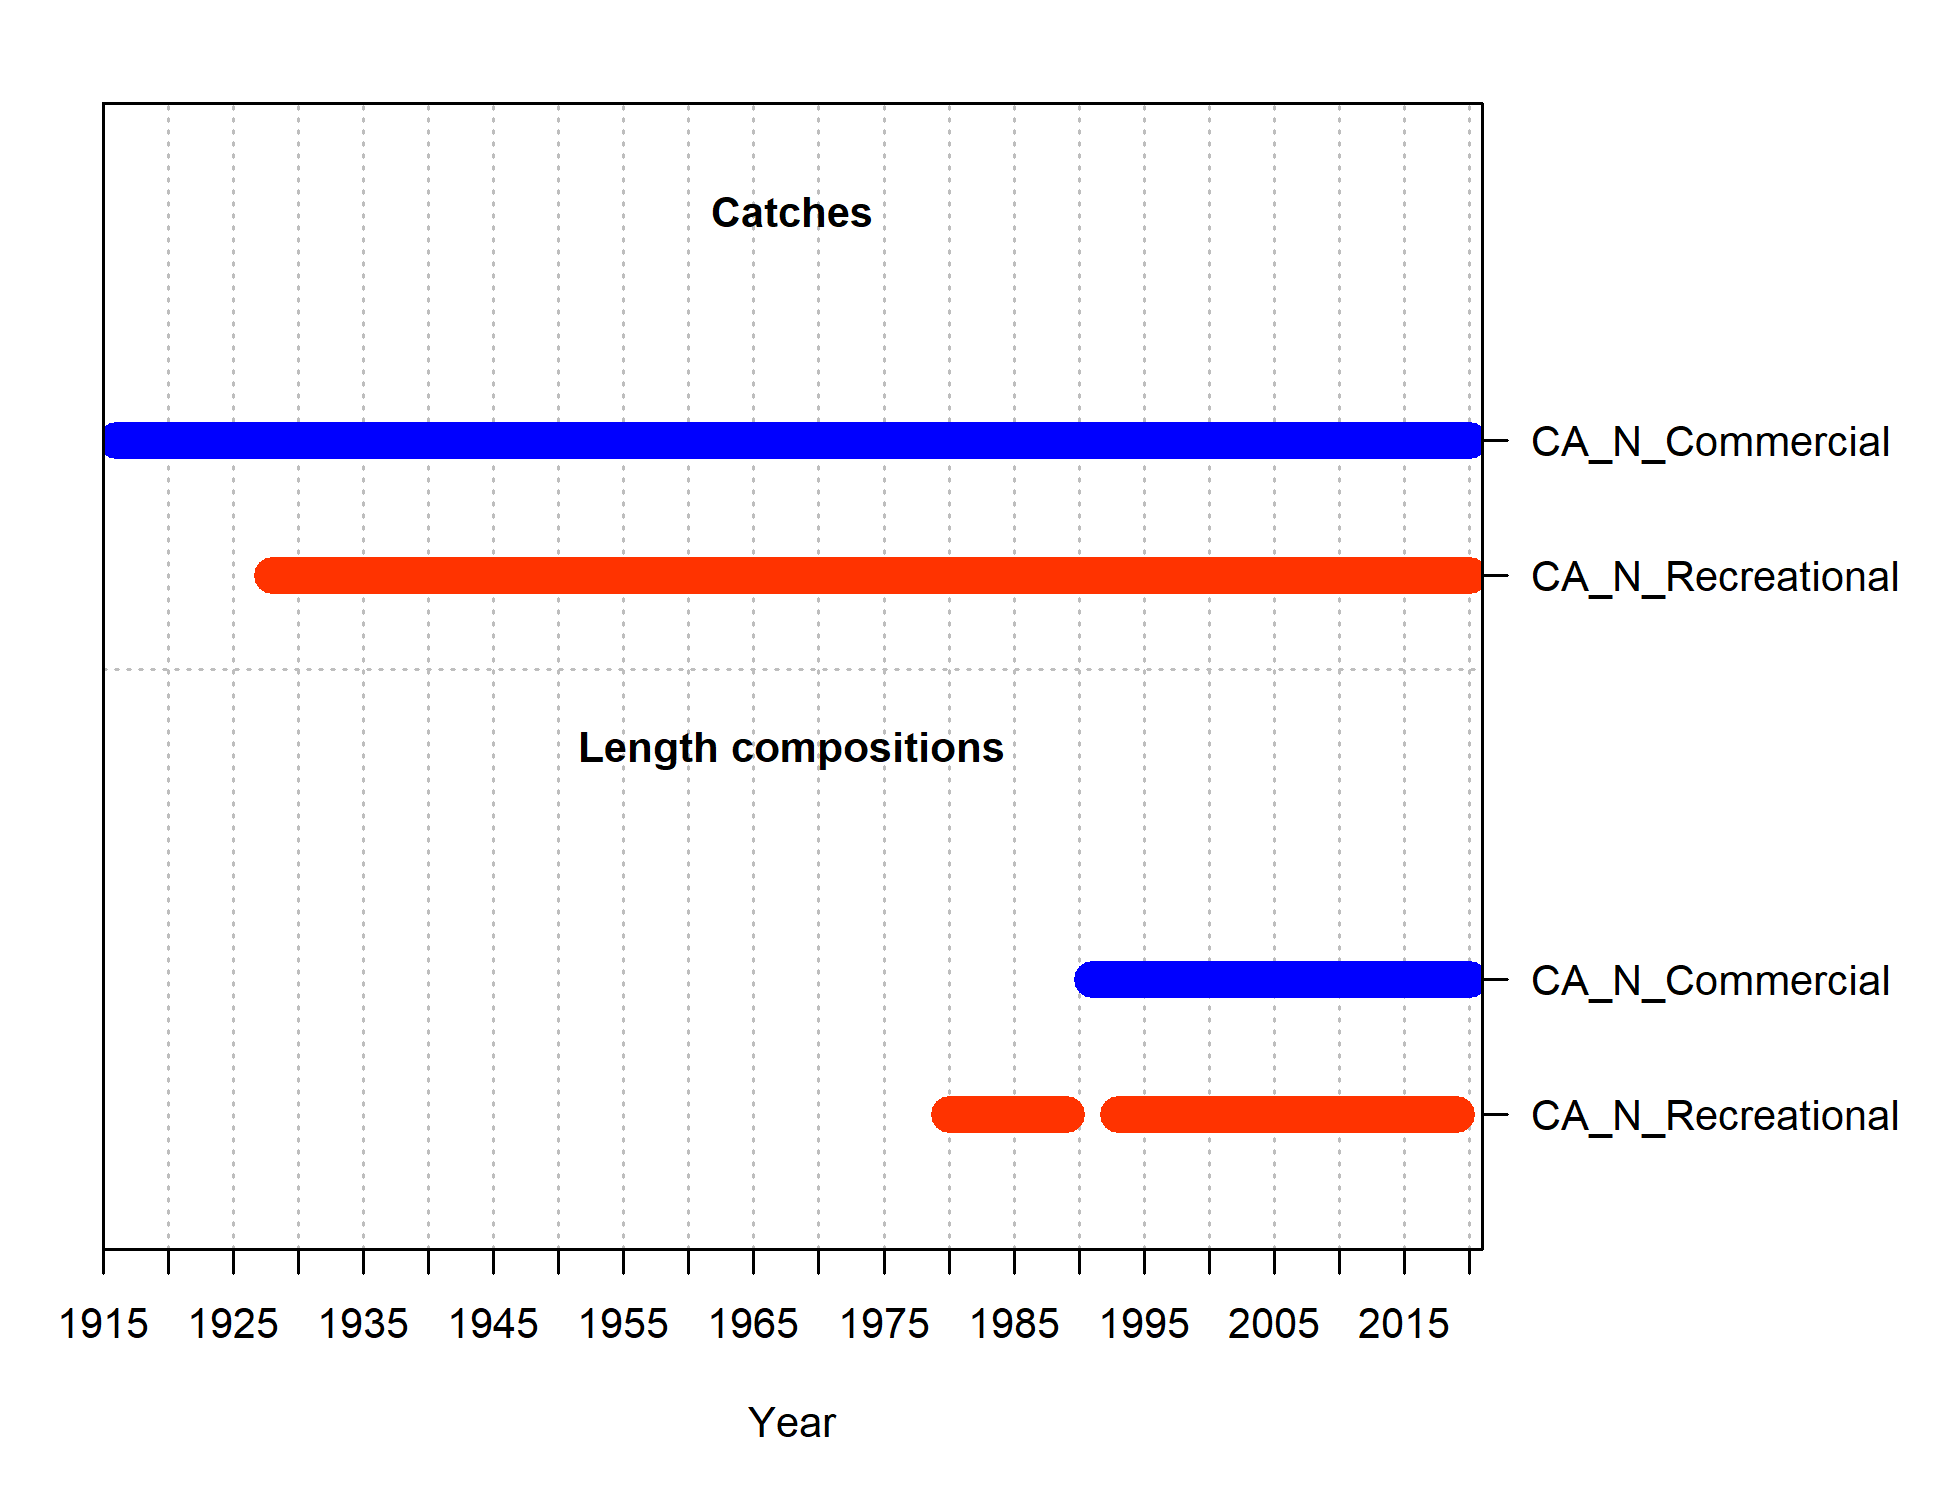
\includegraphics[width=1\textwidth,height=1\textheight]{C:/Assessments/2021/copper_rockfish_2021/write_up/s_ca/figs/data_plot.png}
\caption{Summary of data sources used in the base model.\label{fig:data-plot}}
\end{figure}

\tagmcend\tagstructend

\tagstructbegin{tag=Figure,alttext={.}}\tagmcbegin{tag=Figure}

\begin{figure}
\centering
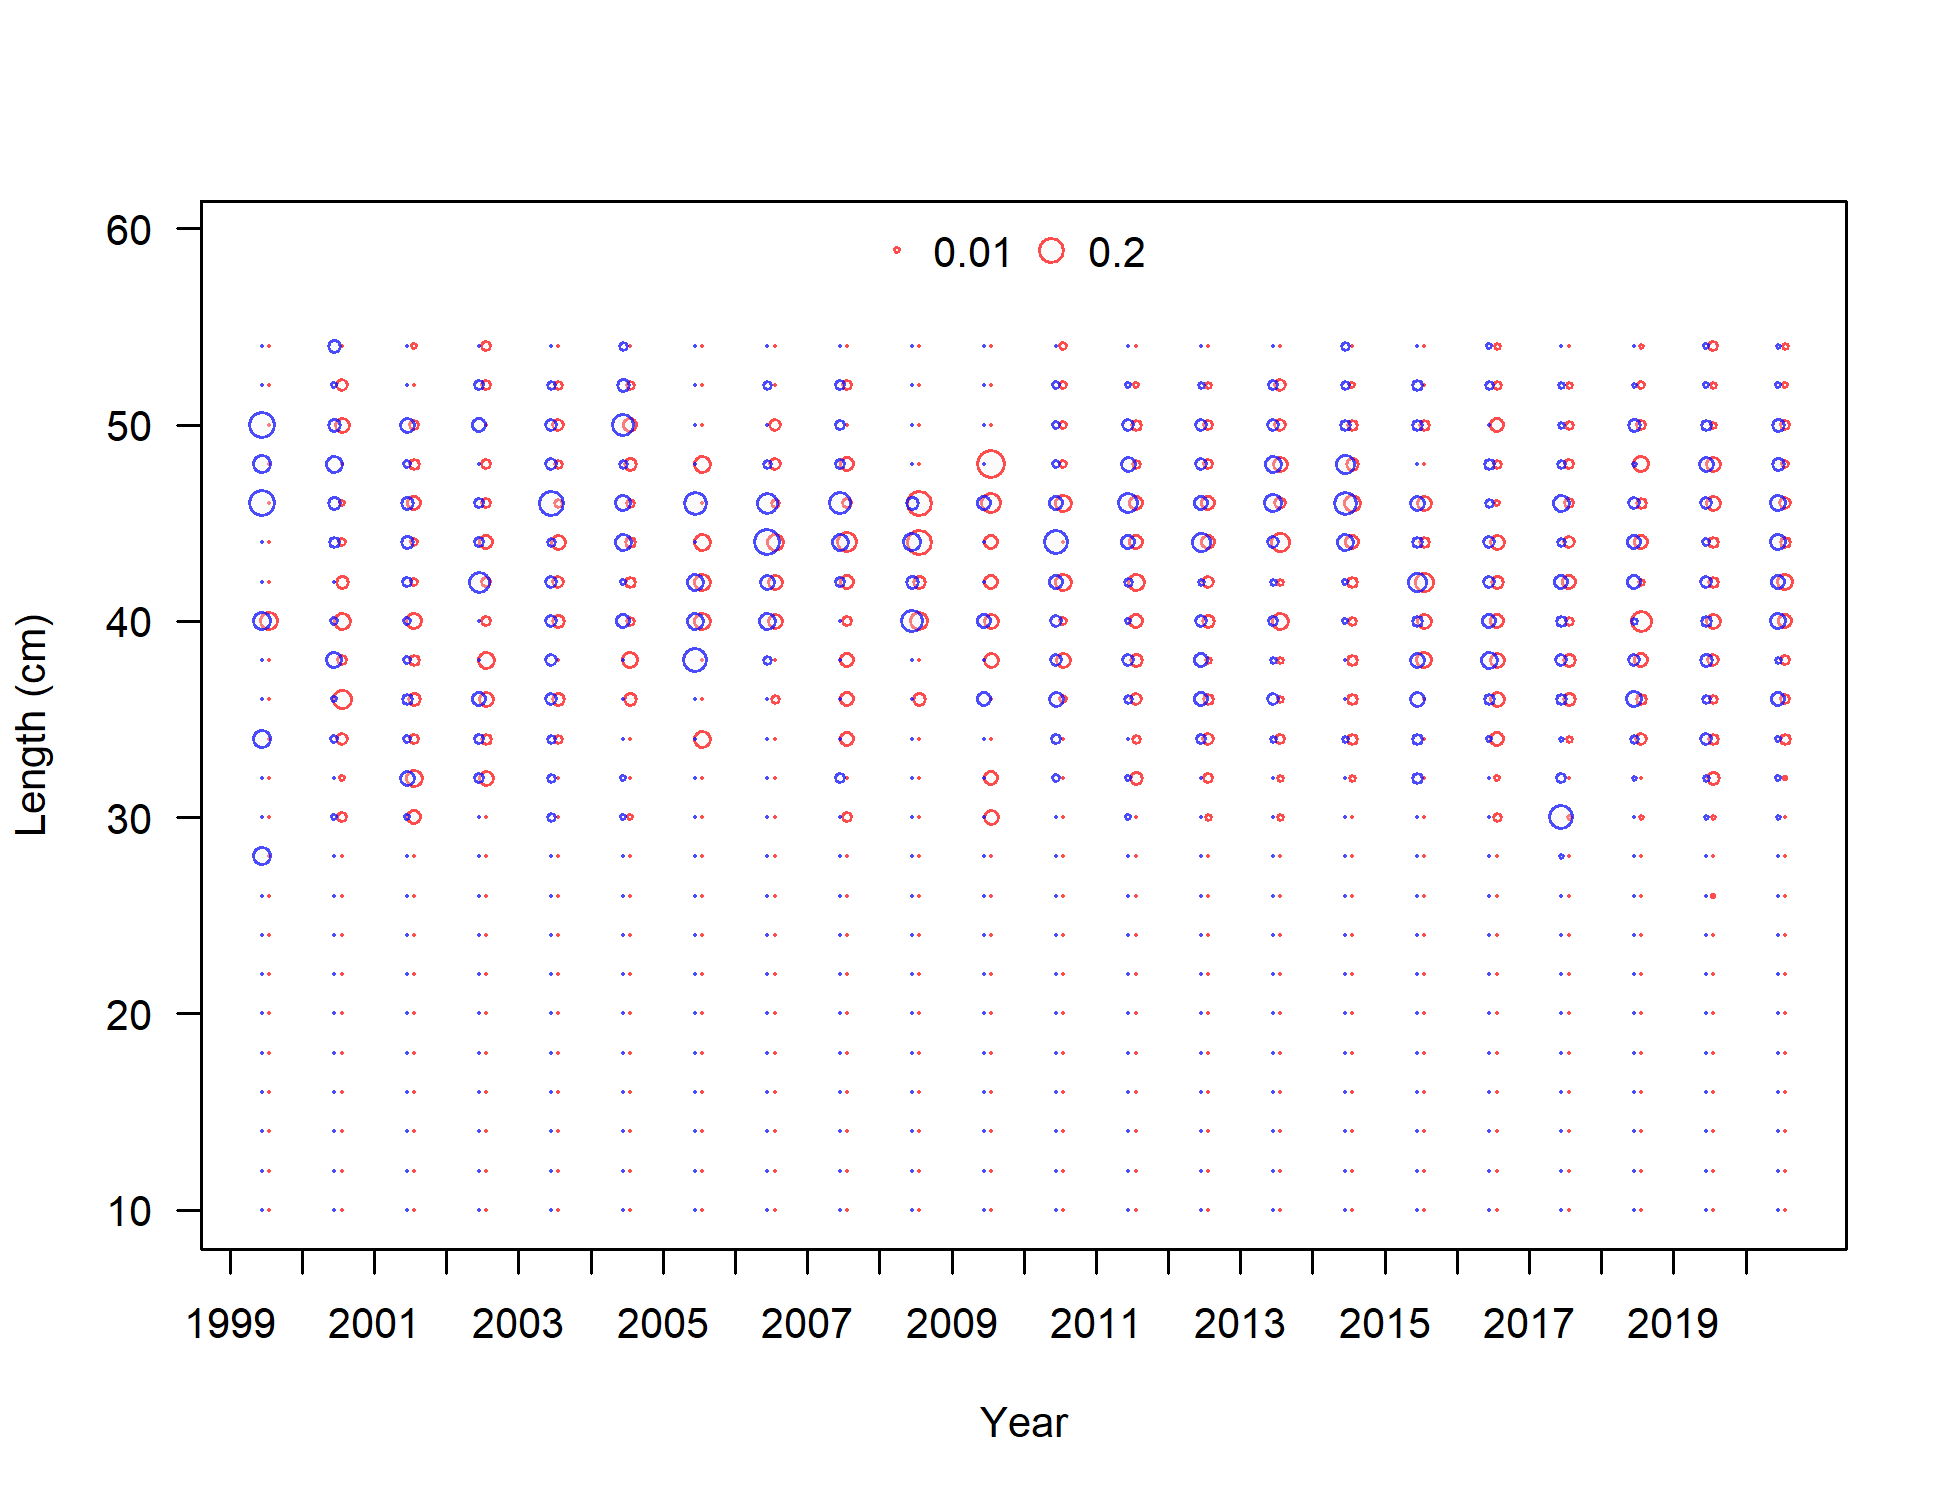
\includegraphics[width=1\textwidth,height=1\textheight]{C:/Assessments/2021/copper_rockfish_2021/models/ca_s_pt_c/12.1_base/plots/comp_lendat_bubflt1mkt0_page2.png}
\caption{Length composition data from the commercial fleet.\label{fig:com-len-data}}
\end{figure}

\tagmcend\tagstructend

\tagstructbegin{tag=Figure,alttext={.}}\tagmcbegin{tag=Figure}

\begin{figure}
\centering
\includegraphics[width=1\textwidth,height=1\textheight]{C:/Assessments/2021/copper_rockfish_2021/models/ca_s_pt_c/12.1_base/plots/comp_lendat_data_weighting_TA1.8_CA_S_Commercial.png}
\caption{Mean length for commercial fleet with 95 percent confidence intervals.\label{fig:mean-com-len-data}}
\end{figure}

\tagmcend\tagstructend

\tagstructbegin{tag=Figure,alttext={.}}\tagmcbegin{tag=Figure}

\begin{figure}
\centering
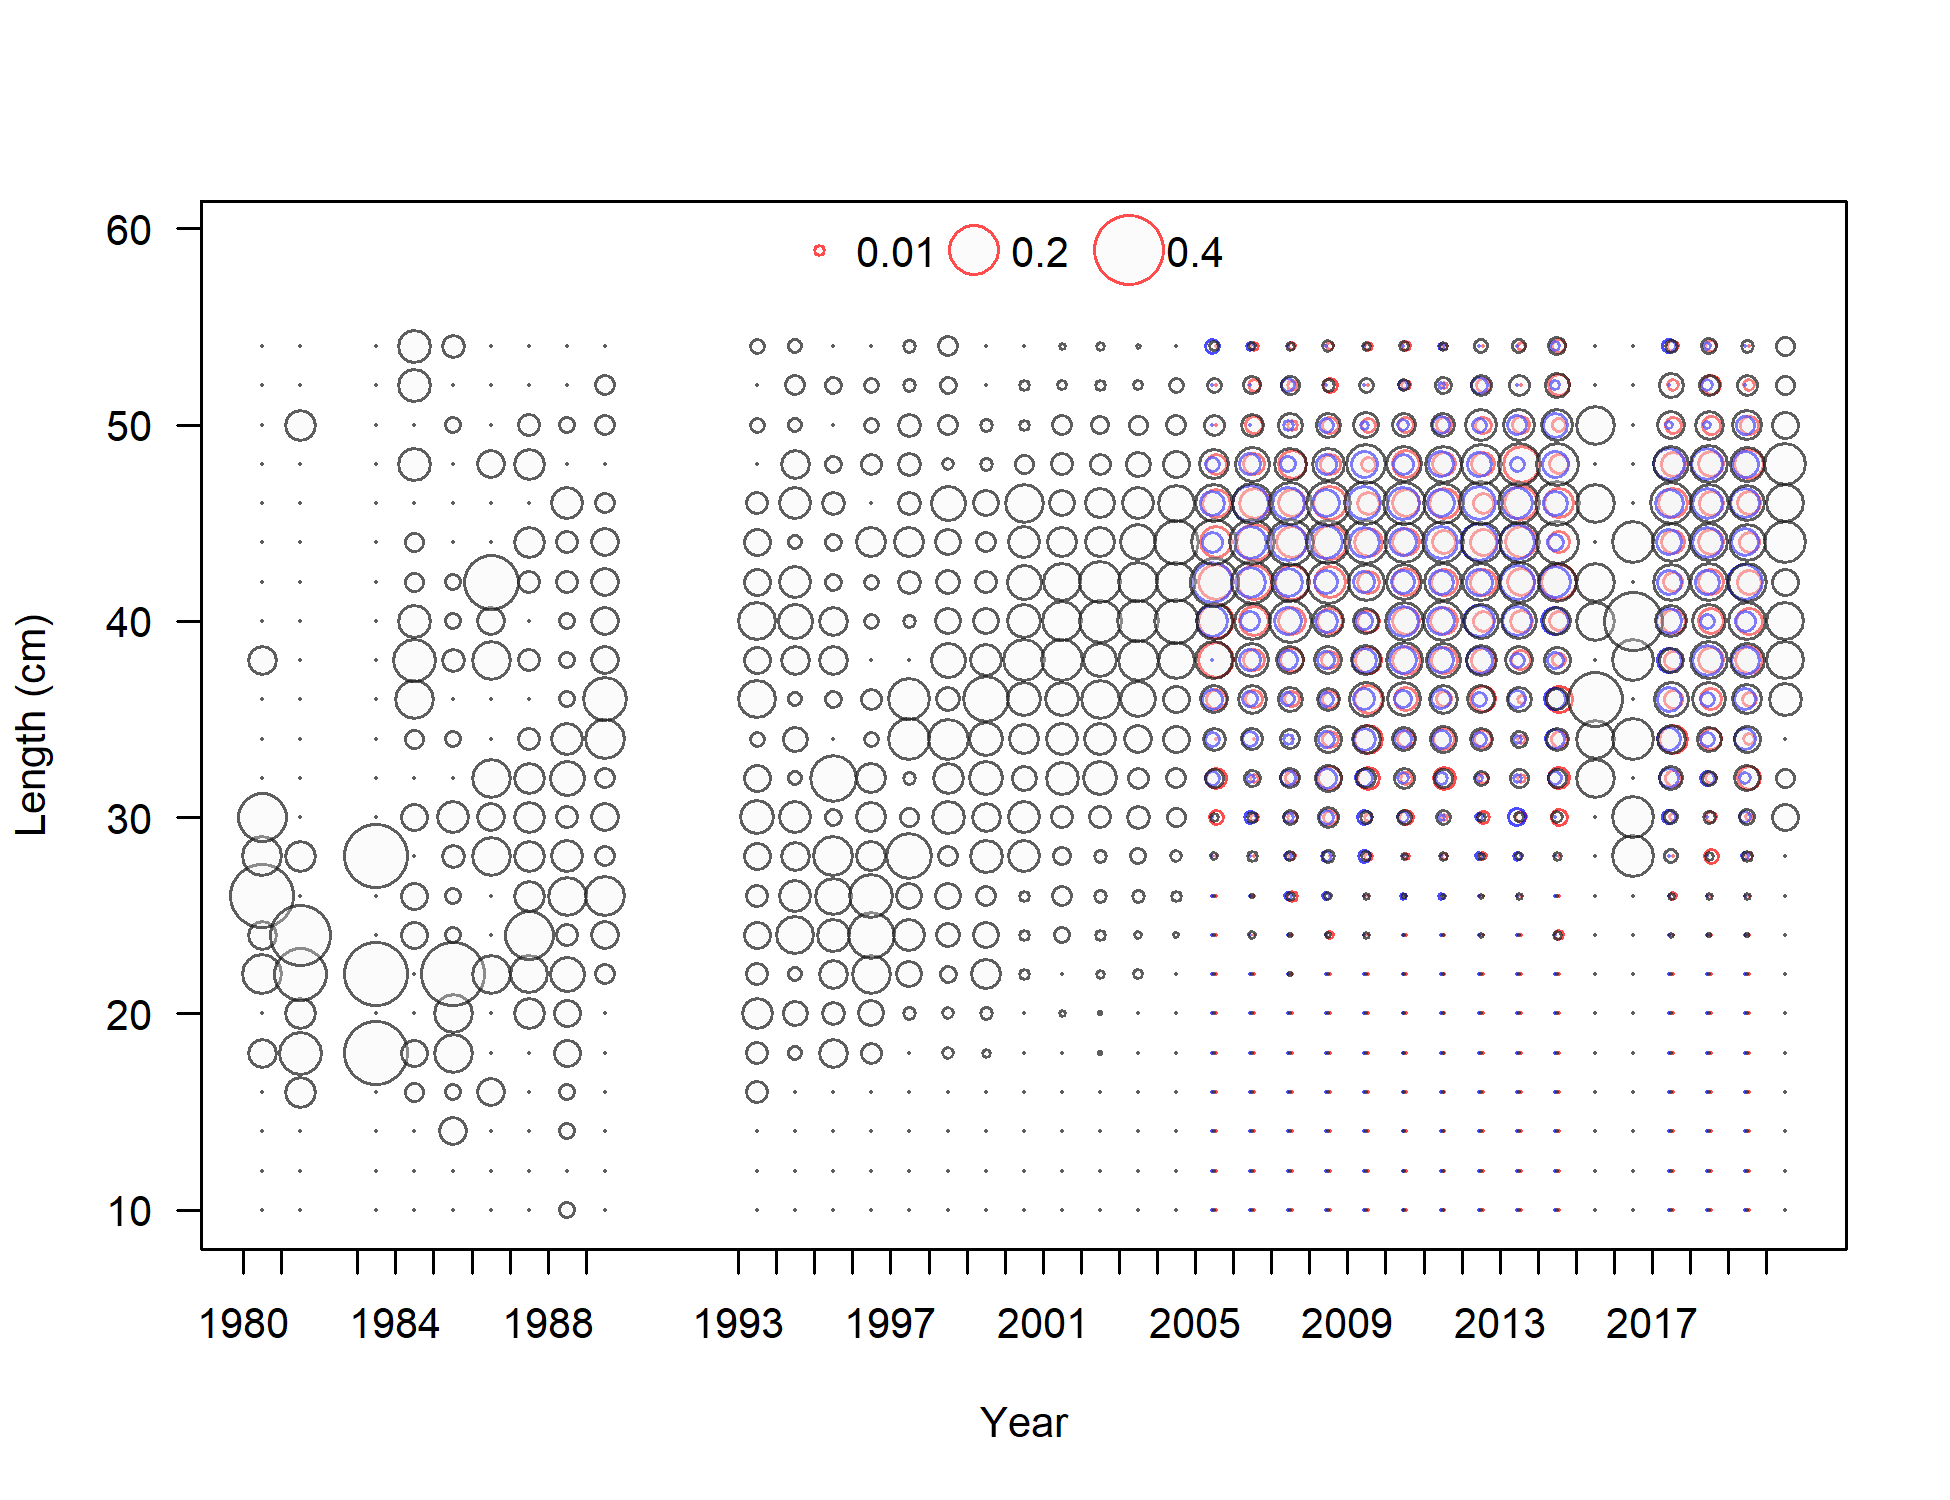
\includegraphics[width=1\textwidth,height=1\textheight]{C:/Assessments/2021/copper_rockfish_2021/models/ca_s_pt_c/12.1_base/plots/comp_lendat_bubflt2mkt0_page3.png}
\caption{Length composition data from the recreational fleet.\label{fig:rec-len-data}}
\end{figure}

\tagmcend\tagstructend

\tagstructbegin{tag=Figure,alttext={.}}\tagmcbegin{tag=Figure}

\begin{figure}
\centering
\includegraphics[width=1\textwidth,height=1\textheight]{C:/Assessments/2021/copper_rockfish_2021/models/ca_s_pt_c/12.1_base/plots/comp_lendat_data_weighting_TA1.8_CA_S_Recreational.png}
\caption{Mean length for recreational fleet with 95 percent confidence intervals.\label{fig:mean-rec-len-data}}
\end{figure}

\tagmcend\tagstructend

\tagstructbegin{tag=Figure,alttext={.}}\tagmcbegin{tag=Figure}

\begin{figure}
\centering
\includegraphics[width=1\textwidth,height=1\textheight]{//nwcfile/FRAM/Assessments/CurrentAssessments/DataModerate_2021/copper_rockfish/data/survey/plots/Map_HL_Sites_lndscp.jpg}
\caption{NWFSC Hook and Line survey sampling sites where yellow sites indicate locations inside Cowcod Conservation Areas. Additionally, known substrate structure, depths, and areas under various management regulations are shown for the area south of Point Conception.\label{fig:hkl-sites}}
\end{figure}

\tagmcend\tagstructend

\tagstructbegin{tag=Figure,alttext={.}}\tagmcbegin{tag=Figure}

\begin{figure}
\centering
\includegraphics[width=1\textwidth,height=1\textheight]{//nwcfile/FRAM/Assessments/CurrentAssessments/DataModerate_2021/copper_rockfish/data/survey/plots/HKL_Site_Observations.png}
\caption{NWFSC Hook and Line survey sample sites inside and outside the CCA and site with observations of copper rockfish.\label{fig:hkl-site-ob}}
\end{figure}

\tagmcend\tagstructend

\tagstructbegin{tag=Figure,alttext={.}}\tagmcbegin{tag=Figure}

\begin{figure}
\centering
\includegraphics[width=1\textwidth,height=1\textheight]{//nwcfile/FRAM/Assessments/CurrentAssessments/DataModerate_2021/copper_rockfish/data/biology/plots/hkl_cca_comparison.png}
\caption{NWFSC Hook and Line survey observations by year outside and inside the cowcod conservation area.\label{fig:hkl-cca}}
\end{figure}

\tagmcend\tagstructend

\tagstructbegin{tag=Figure,alttext={.}}\tagmcbegin{tag=Figure}

\begin{figure}
\centering
\includegraphics[width=1\textwidth,height=1\textheight]{//nwcfile/FRAM/Assessments/CurrentAssessments/DataModerate_2021/copper_rockfish/data/survey/plots/HKL_Size_by_Depth.png}
\caption{Lengths observations by depth in the NWFSC Hook and Line survey data.\label{fig:hkl-len-dep}}
\end{figure}

\tagmcend\tagstructend

\tagstructbegin{tag=Figure,alttext={.}}\tagmcbegin{tag=Figure}

\begin{figure}
\centering
\includegraphics[width=1\textwidth,height=1\textheight]{C:/Assessments/2021/copper_rockfish_2021/models/ca_s_pt_c/12.1_base/plots/comp_lendat_bubflt3mkt0.png}
\caption{Length composition data from the NWFSC Hook and Line survey.\label{fig:hkl-len-data}}
\end{figure}

\tagmcend\tagstructend

\tagstructbegin{tag=Figure,alttext={.}}\tagmcbegin{tag=Figure}

\begin{figure}
\centering
\includegraphics[width=1\textwidth,height=1\textheight]{C:/Assessments/2021/copper_rockfish_2021/models/ca_s_pt_c/12.1_base/plots/comp_lendat_data_weighting_TA1.8_NWFSC_HKL.png}
\caption{Mean length for NWFSC Hook and Line survey with 95 percent confidence intervals.\label{fig:mean-hkl-len-data}}
\end{figure}

\tagmcend\tagstructend

\tagstructbegin{tag=Figure,alttext={.}}\tagmcbegin{tag=Figure}

\begin{figure}
\centering
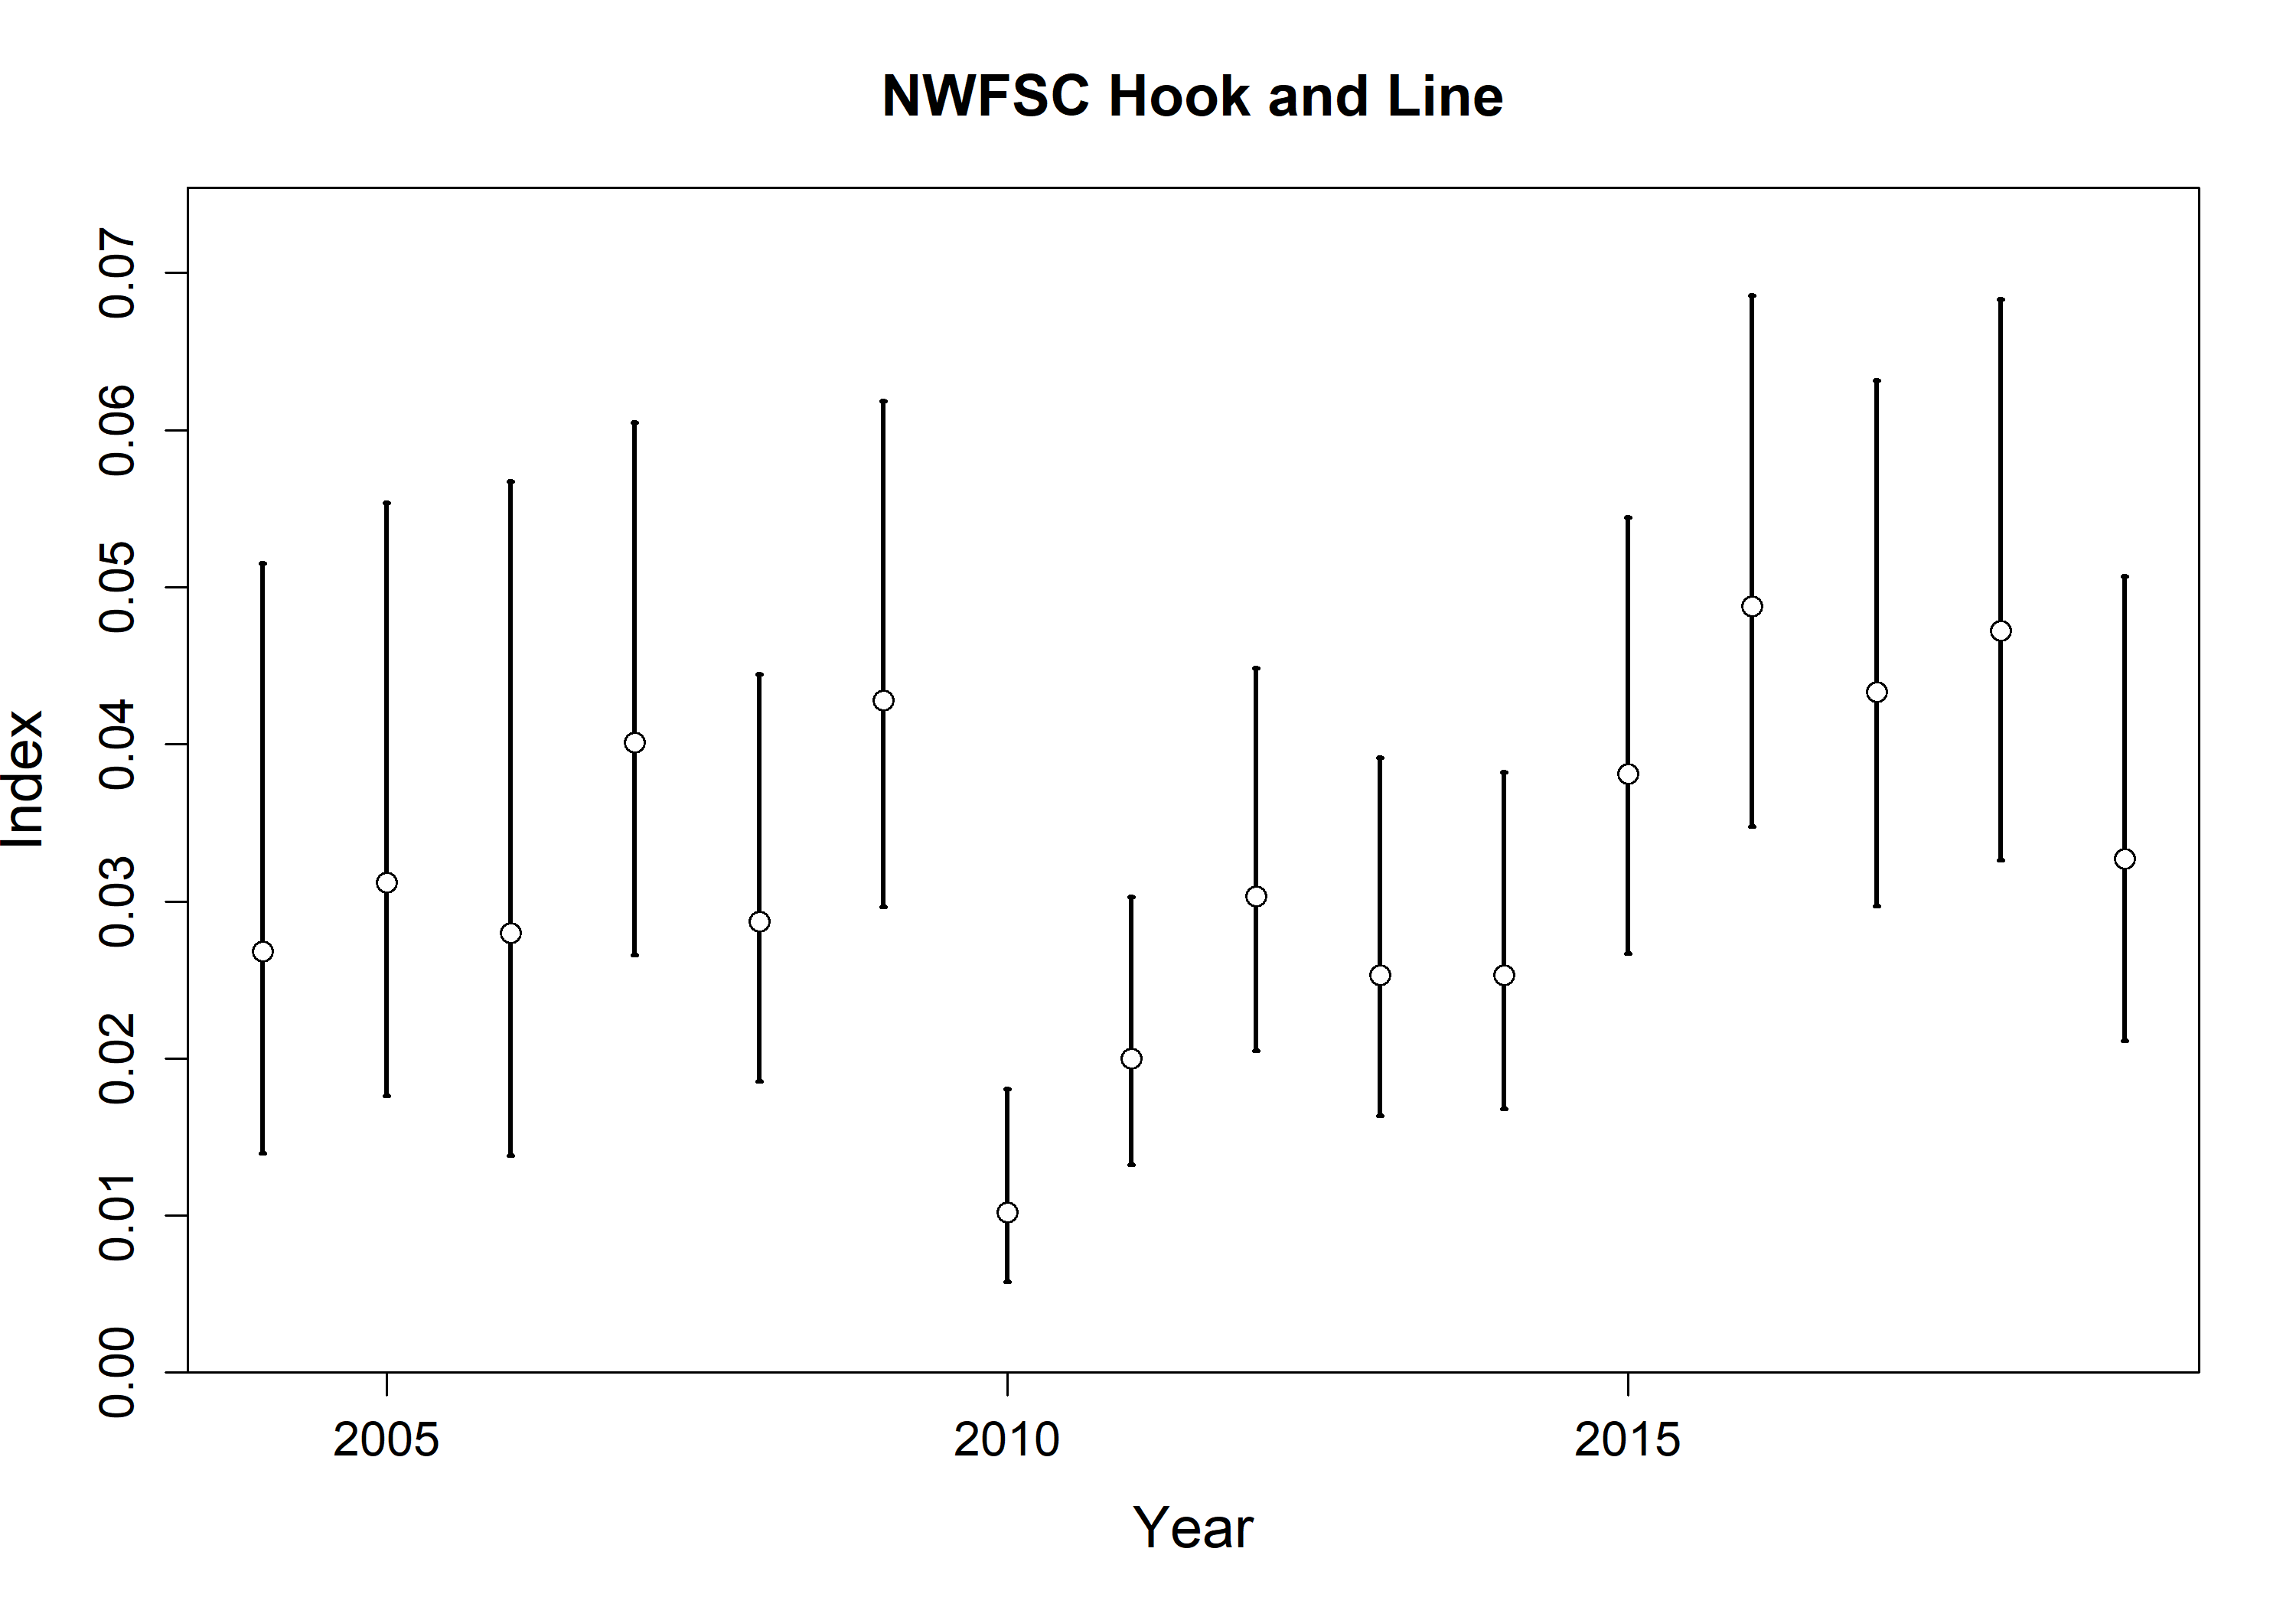
\includegraphics[width=1\textwidth,height=1\textheight]{C:/Assessments/2021/copper_rockfish_2021/write_up/s_ca/figs/hkl_index.png}
\caption{Index of abundance for the NWFSC Hook and Line survey. Lines indicate 95 percent uncertainty interval around index values based on the model assumption of lognormal error. Thicker lines indicate input uncertainty before addition of estimated additional uncertainty parameter.\label{fig:hkl-index}}
\end{figure}

\tagmcend\tagstructend

\tagstructbegin{tag=Figure,alttext={.}}\tagmcbegin{tag=Figure}

\begin{figure}
\centering
\includegraphics[width=1\textwidth,height=1\textheight]{//nwcfile/FRAM/Assessments/CurrentAssessments/DataModerate_2021/copper_rockfish/data/survey_indices/Copp.2019.NFT.1m.ALL/Copp.ALL.GAM.Fig.png}
\caption{Diagnostics for the binomial generalized-linear model.\label{fig:hkl-diag}}
\end{figure}

\tagmcend\tagstructend

\tagstructbegin{tag=Figure,alttext={.}}\tagmcbegin{tag=Figure}

\begin{figure}
\centering
\includegraphics[width=1\textwidth,height=1\textheight]{//nwcfile/FRAM/Assessments/CurrentAssessments/DataModerate_2021/copper_rockfish/data/biology/plots/doc_Length_Weight_Source.png}
\caption{Comparison of the length-at-weight data from the NWFSC Hook and Line and the NWFSC WCGBT surveys.\label{fig:len-weight-survey}}
\end{figure}

\tagmcend\tagstructend

\tagstructbegin{tag=Figure,alttext={.}}\tagmcbegin{tag=Figure}

\begin{figure}
\centering
\includegraphics[width=1\textwidth,height=1\textheight]{//nwcfile/FRAM/Assessments/CurrentAssessments/DataModerate_2021/copper_rockfish/data/biology/plots/doc_Length_Weight_Sex.png}
\caption{All available survey length-at-weight data with sex specific estimated fits.\label{fig:len-weight}}
\end{figure}

\tagmcend\tagstructend

\tagstructbegin{tag=Figure,alttext={.}}\tagmcbegin{tag=Figure}

\begin{figure}
\centering
\includegraphics[width=1\textwidth,height=1\textheight]{//nwcfile/FRAM/Assessments/CurrentAssessments/DataModerate_2021/copper_rockfish/data/biology/plots/South_Len_at_Age.png}
\caption{Length-at-age for non-randomly sampled larger fish observed by the NWFSC Hook and Line and WCGBT surveys.\label{fig:survey-len-at-age-data}}
\end{figure}

\tagmcend\tagstructend

\tagstructbegin{tag=Figure,alttext={.}}\tagmcbegin{tag=Figure}

\begin{figure}
\centering
\includegraphics[width=1\textwidth,height=1\textheight]{//nwcfile/FRAM/Assessments/CurrentAssessments/DataModerate_2021/copper_rockfish/data/biology/plots/doc_south_Age_by_Sex_Source.png}
\caption{Length-at-age for non-randomly sampled larger fish observed by the NWFSC Hook and Line and WCGBT surveys and young fish from Lea.\label{fig:south-len-at-age-data}}
\end{figure}

\tagmcend\tagstructend

\tagstructbegin{tag=Figure,alttext={.}}\tagmcbegin{tag=Figure}

\begin{figure}
\centering
\includegraphics[width=1\textwidth,height=1\textheight]{//nwcfile/FRAM/Assessments/CurrentAssessments/DataModerate_2021/copper_rockfish/data/biology/plots/South_Data_Comparison_Len_at_Age.png}
\caption{Length-at-age comparisons between survey collected fish south of Point Conception and to those observed off the coast of Oregon and Washington.\label{fig:len-at-age-comp}}
\end{figure}

\tagmcend\tagstructend

\clearpage

\tagstructbegin{tag=Figure,alttext={.}}\tagmcbegin{tag=Figure}

\begin{figure}
\centering
\includegraphics[width=1\textwidth,height=1\textheight]{C:/Assessments/2021/copper_rockfish_2021/models/ca_s_pt_c/12.1_base/plots/bio1_sizeatage.png}
\caption{Length-at-age in the beginning of the year with the coefficient of variation by age within the model.\label{fig:len-age-ss}}
\end{figure}

\tagmcend\tagstructend

\tagstructbegin{tag=Figure,alttext={.}}\tagmcbegin{tag=Figure}

\begin{figure}
\centering
\includegraphics[width=1\textwidth,height=1\textheight]{C:/Assessments/2021/copper_rockfish_2021/models/ca_s_pt_c/12.1_base/plots/bio6_maturity.png}
\caption{Maturity as a function of length.\label{fig:maturity}}
\end{figure}

\tagmcend\tagstructend

\tagstructbegin{tag=Figure,alttext={.}}\tagmcbegin{tag=Figure}

\begin{figure}
\centering
\includegraphics[width=1\textwidth,height=1\textheight]{C:/Assessments/2021/copper_rockfish_2021/models/ca_s_pt_c/12.1_base/plots/bio9_fecundity_len.png}
\caption{Fecundity as a function of length.\label{fig:fecundity}}
\end{figure}

\tagmcend\tagstructend

\tagstructbegin{tag=Figure,alttext={.}}\tagmcbegin{tag=Figure}

\begin{figure}
\centering
\includegraphics[width=1\textwidth,height=1\textheight]{//nwcfile/FRAM/Assessments/CurrentAssessments/DataModerate_2021/copper_rockfish/data/biology/plots/Length_fraction_female.png}
\caption{Fraction female by length across all available data sources.\label{fig:len-sex-ratio}}
\end{figure}

\tagmcend\tagstructend

\tagstructbegin{tag=Figure,alttext={.}}\tagmcbegin{tag=Figure}

\begin{figure}
\centering
\includegraphics[width=1\textwidth,height=1\textheight]{//nwcfile/FRAM/Assessments/CurrentAssessments/DataModerate_2021/copper_rockfish/data/biology/plots/Age_fraction_female.png}
\caption{Fraction female by age across all available data sources.\label{fig:age-sex-ratio}}
\end{figure}

\tagmcend\tagstructend

\tagstructbegin{tag=Figure,alttext={.}}\tagmcbegin{tag=Figure}

\begin{figure}
\centering
\includegraphics[width=1\textwidth,height=1\textheight]{C:/Assessments/2021/copper_rockfish_2021/models/ca_s_pt_c/_bridge/_plots/Initial_Bridge.png}
\caption{Comparison between SS bridge model and the results from the 2013 XDB-SRA model.\label{fig:bridge-1}}
\end{figure}

\tagmcend\tagstructend

\tagstructbegin{tag=Figure,alttext={.}}\tagmcbegin{tag=Figure}

\begin{figure}
\centering
\includegraphics[width=1\textwidth,height=1\textheight]{C:/Assessments/2021/copper_rockfish_2021/models/ca_s_pt_c/_bridge/_plots/Growth.png}
\caption{Adjustment to SS female weight-at-length curve to create a match in stock scale to XDB-SRA.\label{fig:bridge-growth}}
\end{figure}

\tagmcend\tagstructend

\tagstructbegin{tag=Figure,alttext={.}}\tagmcbegin{tag=Figure}

\begin{figure}
\centering
\includegraphics[width=1\textwidth,height=1\textheight]{C:/Assessments/2021/copper_rockfish_2021/models/ca_s_pt_c/_bridge/_plots/1_bridge_all_compare1_spawnbio.png}
\caption{The time series of spawning biomass (or output) for updates to the 2013 model.\label{fig:bridge-ssb}}
\end{figure}

\tagmcend\tagstructend

\tagstructbegin{tag=Figure,alttext={.}}\tagmcbegin{tag=Figure}

\begin{figure}
\centering
\includegraphics[width=1\textwidth,height=1\textheight]{C:/Assessments/2021/copper_rockfish_2021/models/ca_s_pt_c/_bridge/_plots/1_bridge_all_compare3_Bratio.png}
\caption{The time series of fraction unfished for updates to the 2013 model.\label{fig:bridge-depl}}
\end{figure}

\tagmcend\tagstructend

\tagstructbegin{tag=Figure,alttext={.}}\tagmcbegin{tag=Figure}

\begin{figure}
\centering
\includegraphics[width=1\textwidth,height=1\textheight]{C:/Assessments/2021/copper_rockfish_2021/models/ca_s_pt_c/_bridge/_plots/1_bridge_subset_compare1_spawnbio.png}
\caption{The time series of spawning output for the subset of bridge models with the updated fecundity relationship.\label{fig:bridge-ssb-2}}
\end{figure}

\tagmcend\tagstructend

\tagstructbegin{tag=Figure,alttext={.}}\tagmcbegin{tag=Figure}

\begin{figure}
\centering
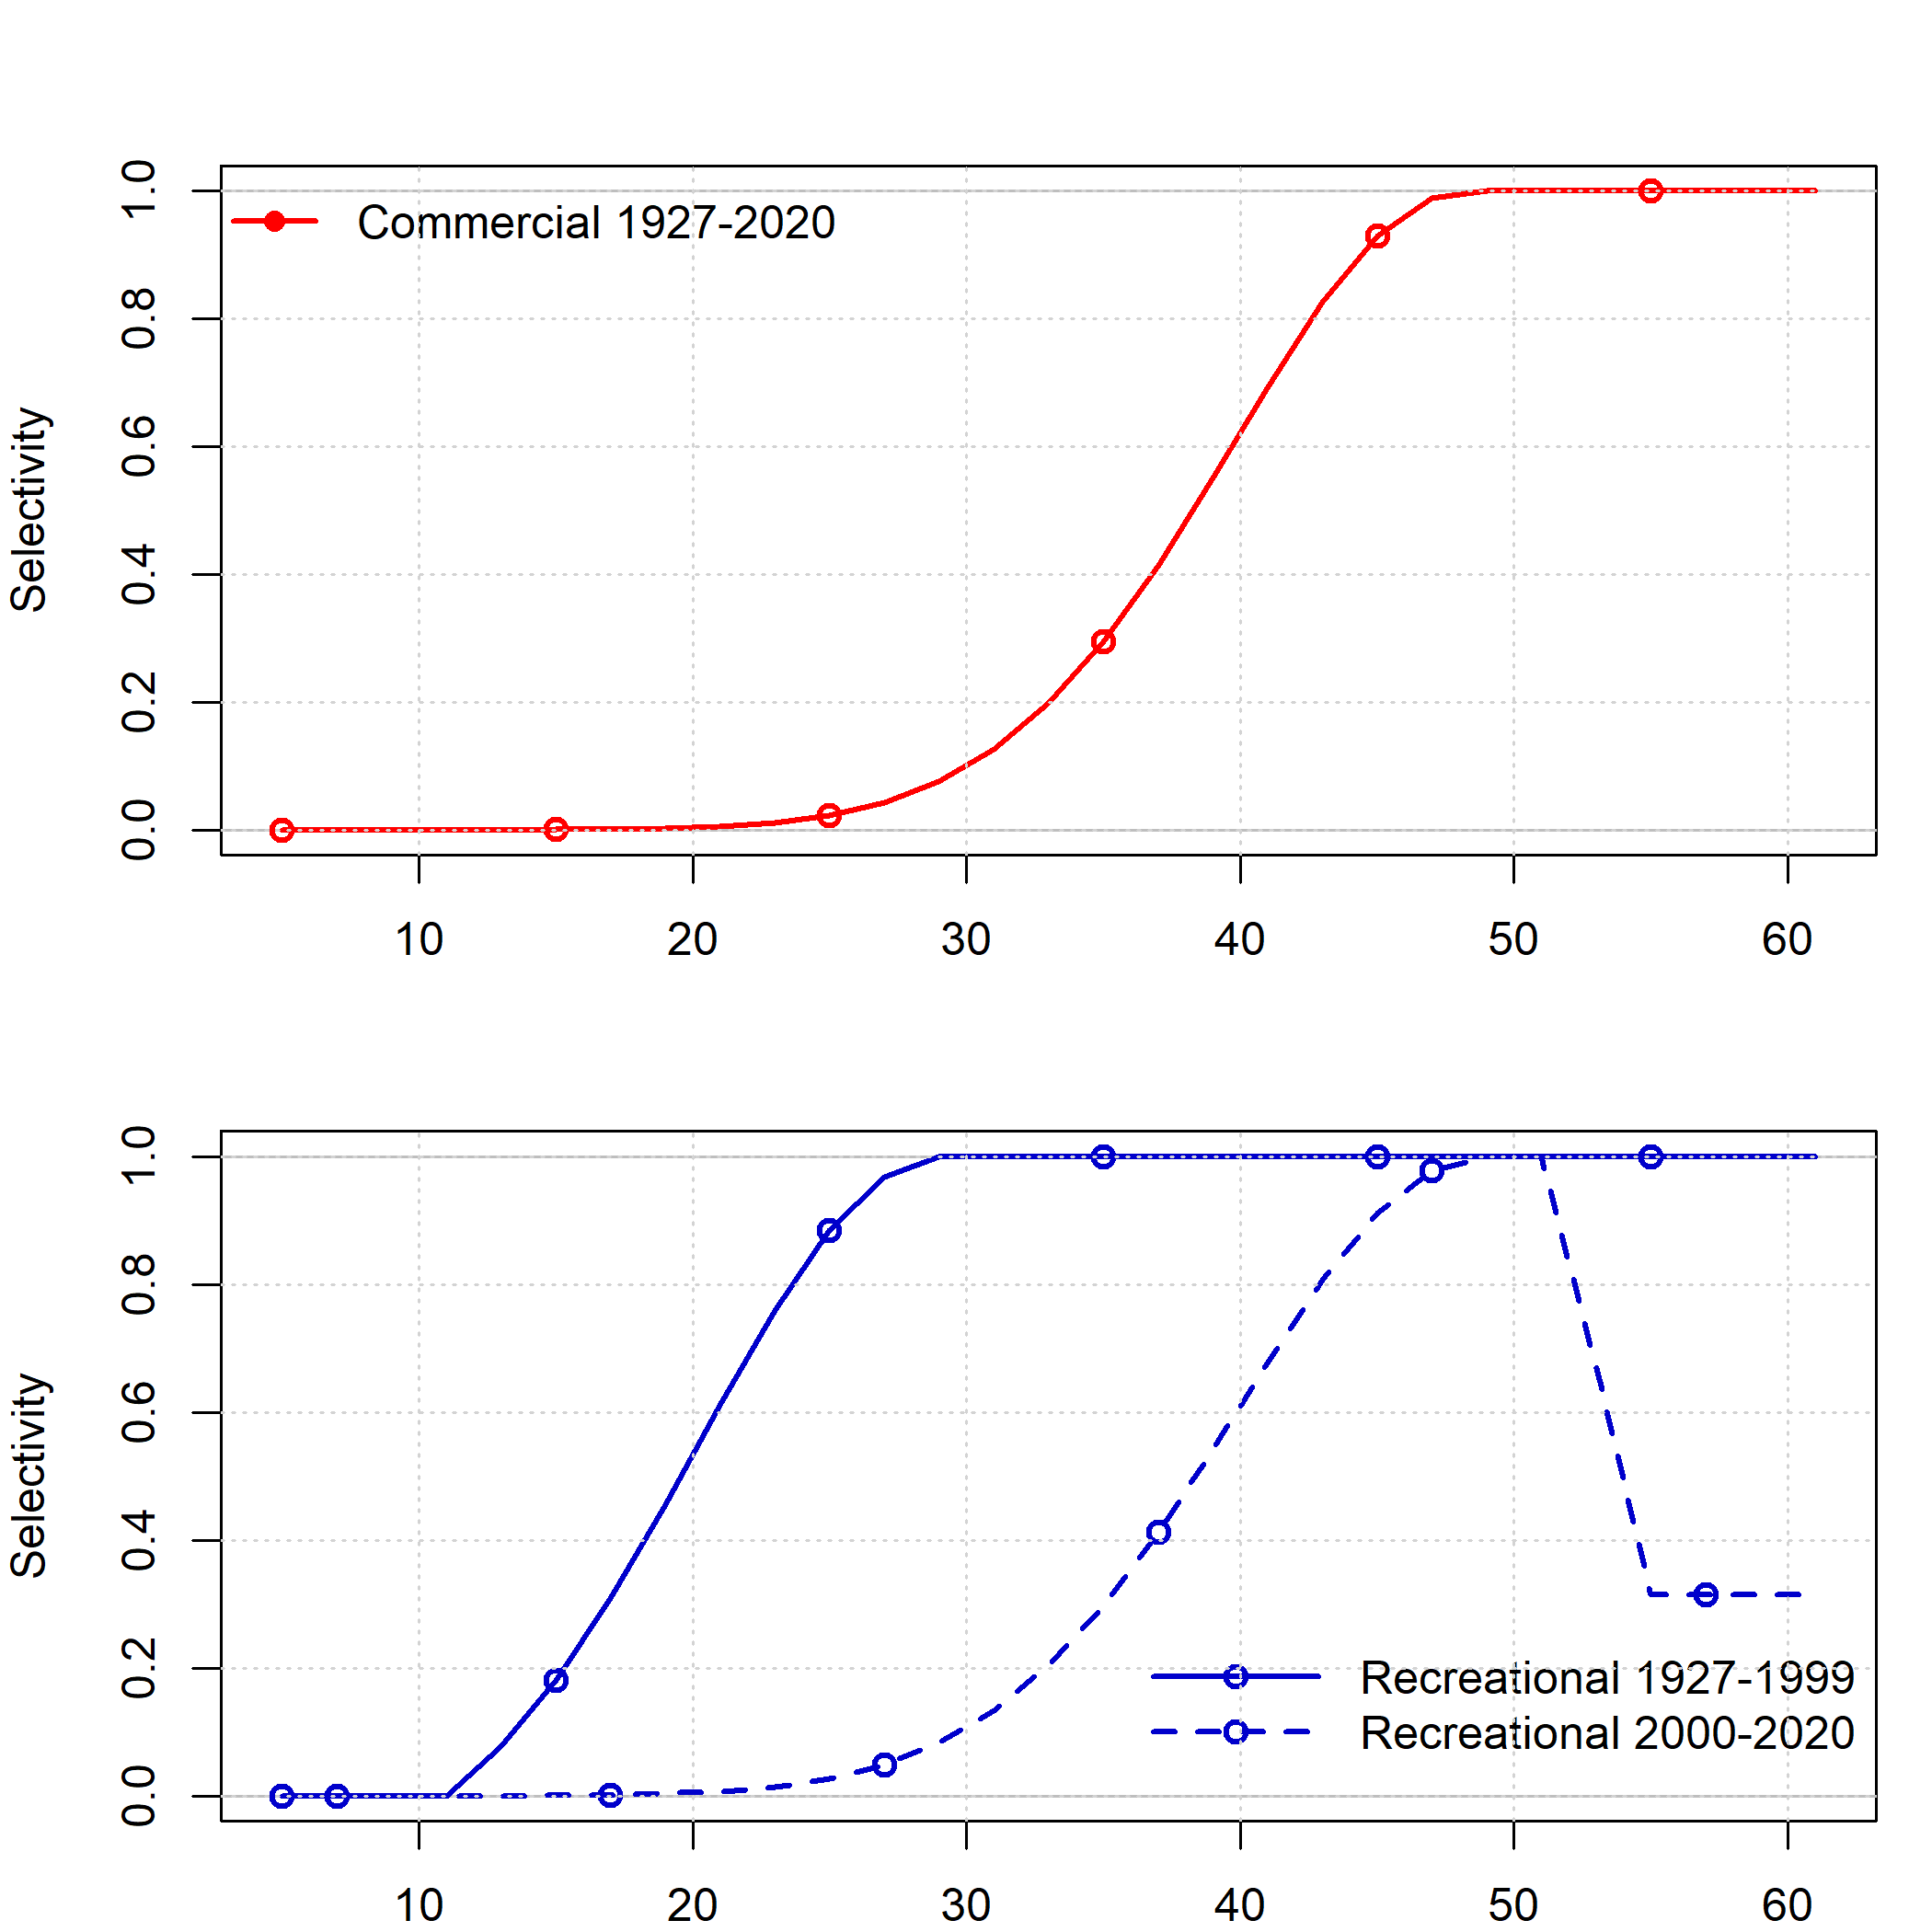
\includegraphics[width=1\textwidth,height=1\textheight]{C:/Assessments/2021/copper_rockfish_2021/write_up/s_ca/figs/selectivity.png}
\caption{Selectivity at length by fleet.\label{fig:selex}}
\end{figure}

\tagmcend\tagstructend

\tagstructbegin{tag=Figure,alttext={.}}\tagmcbegin{tag=Figure}

\begin{figure}
\centering
\includegraphics[width=1\textwidth,height=1\textheight]{//nwcfile/FRAM/Assessments/CurrentAssessments/DataModerate_2021/copper_rockfish/models/ca_s_pt_c/10.0_base_retro/Squid_RecDevs.png}
\caption{The estimated recruitment deviations as additional years of data are removed during a retrospective run. Select years of estimated recruitment deviations remain greater than 0 after all informative data are removed.\label{fig:squid-rec}}
\end{figure}

\tagmcend\tagstructend

\tagstructbegin{tag=Figure,alttext={.}}\tagmcbegin{tag=Figure}

\begin{figure}
\centering
\includegraphics[width=1\textwidth,height=1\textheight]{C:/Assessments/2021/copper_rockfish_2021/models/ca_s_pt_c/12.1_base/plots/SR_curve.png}
\caption{Stock-recruit curve. Point colors indicate year, with warmer colors indicating earlier years and cooler colors in showing later years.\label{fig:bh-curve}}
\end{figure}

\tagmcend\tagstructend

\tagstructbegin{tag=Figure,alttext={.}}\tagmcbegin{tag=Figure}

\begin{figure}
\centering
\includegraphics[width=1\textwidth,height=1\textheight]{C:/Assessments/2021/copper_rockfish_2021/models/ca_s_pt_c/12.1_base/plots/ts11_Age-0_recruits_(1000s)_with_95_asymptotic_intervals.png}
\caption{Estimated time series of age-0 recruits (1000s).\label{fig:recruits}}
\end{figure}

\tagmcend\tagstructend

\tagstructbegin{tag=Figure,alttext={.}}\tagmcbegin{tag=Figure}

\begin{figure}
\centering
\includegraphics[width=1\textwidth,height=1\textheight]{C:/Assessments/2021/copper_rockfish_2021/models/ca_s_pt_c/12.1_base/plots/comp_lenfit_residsflt1mkt0_page2.png}
\caption{Pearson residuals for commercial fleet. Closed bubble are positive residuals (observed \textgreater{} expected) and open bubbles are negative residuals (observed \textless{} expected).\label{fig:com-pearson}}
\end{figure}

\tagmcend\tagstructend

\tagstructbegin{tag=Figure,alttext={.}}\tagmcbegin{tag=Figure}

\begin{figure}
\centering
\includegraphics[width=1\textwidth,height=1\textheight]{C:/Assessments/2021/copper_rockfish_2021/models/ca_s_pt_c/12.1_base/plots/comp_lenfit_data_weighting_TA1.8_CA_S_Commercial.png}
\caption{Mean length for commercial lengths with 95 percent confidence intervals based on current samples sizes.\label{fig:com-mean-len-fit}}
\end{figure}

\tagmcend\tagstructend

\tagstructbegin{tag=Figure,alttext={.}}\tagmcbegin{tag=Figure}

\begin{figure}
\centering
\includegraphics[width=1\textwidth,height=1\textheight]{C:/Assessments/2021/copper_rockfish_2021/models/ca_s_pt_c/12.1_base/plots/comp_lenfit_residsflt2mkt0_page3.png}
\caption{Pearson residuals for recreational fleet. Closed bubble are positive residuals (observed \textgreater{} expected) and open bubbles are negative residuals (observed \textless{} expected).\label{fig:rec-pearson}}
\end{figure}

\tagmcend\tagstructend

\tagstructbegin{tag=Figure,alttext={.}}\tagmcbegin{tag=Figure}

\begin{figure}
\centering
\includegraphics[width=1\textwidth,height=1\textheight]{C:/Assessments/2021/copper_rockfish_2021/models/ca_s_pt_c/12.1_base/plots/comp_lenfit_data_weighting_TA1.8_CA_S_Recreational.png}
\caption{Mean length for recreational lengths with 95 percent confidence intervals based on current samples sizes.\label{fig:rec-mean-len-fit}}
\end{figure}

\tagmcend\tagstructend

\tagstructbegin{tag=Figure,alttext={.}}\tagmcbegin{tag=Figure}

\begin{figure}
\centering
\includegraphics[width=1\textwidth,height=1\textheight]{C:/Assessments/2021/copper_rockfish_2021/models/ca_s_pt_c/12.1_base/plots/comp_lenfit_residsflt3mkt0.png}
\caption{Pearson residuals for NWFSC Hook and Line survey. Closed bubble are positive residuals (observed \textgreater{} expected) and open bubbles are negative residuals (observed \textless{} expected).\label{fig:hkl-pearson}}
\end{figure}

\tagmcend\tagstructend

\tagstructbegin{tag=Figure,alttext={.}}\tagmcbegin{tag=Figure}

\begin{figure}
\centering
\includegraphics[width=1\textwidth,height=1\textheight]{C:/Assessments/2021/copper_rockfish_2021/models/ca_s_pt_c/12.1_base/plots/comp_lenfit_data_weighting_TA1.8_NWFSC_HKL.png}
\caption{Mean length for NWFSC Hook and Line survey lengths with 95 percent confidence intervals based on current samples sizes.\label{fig:hkl-mean-len-fit}}
\end{figure}

\tagmcend\tagstructend

\tagstructbegin{tag=Figure,alttext={.}}\tagmcbegin{tag=Figure}

\begin{figure}
\centering
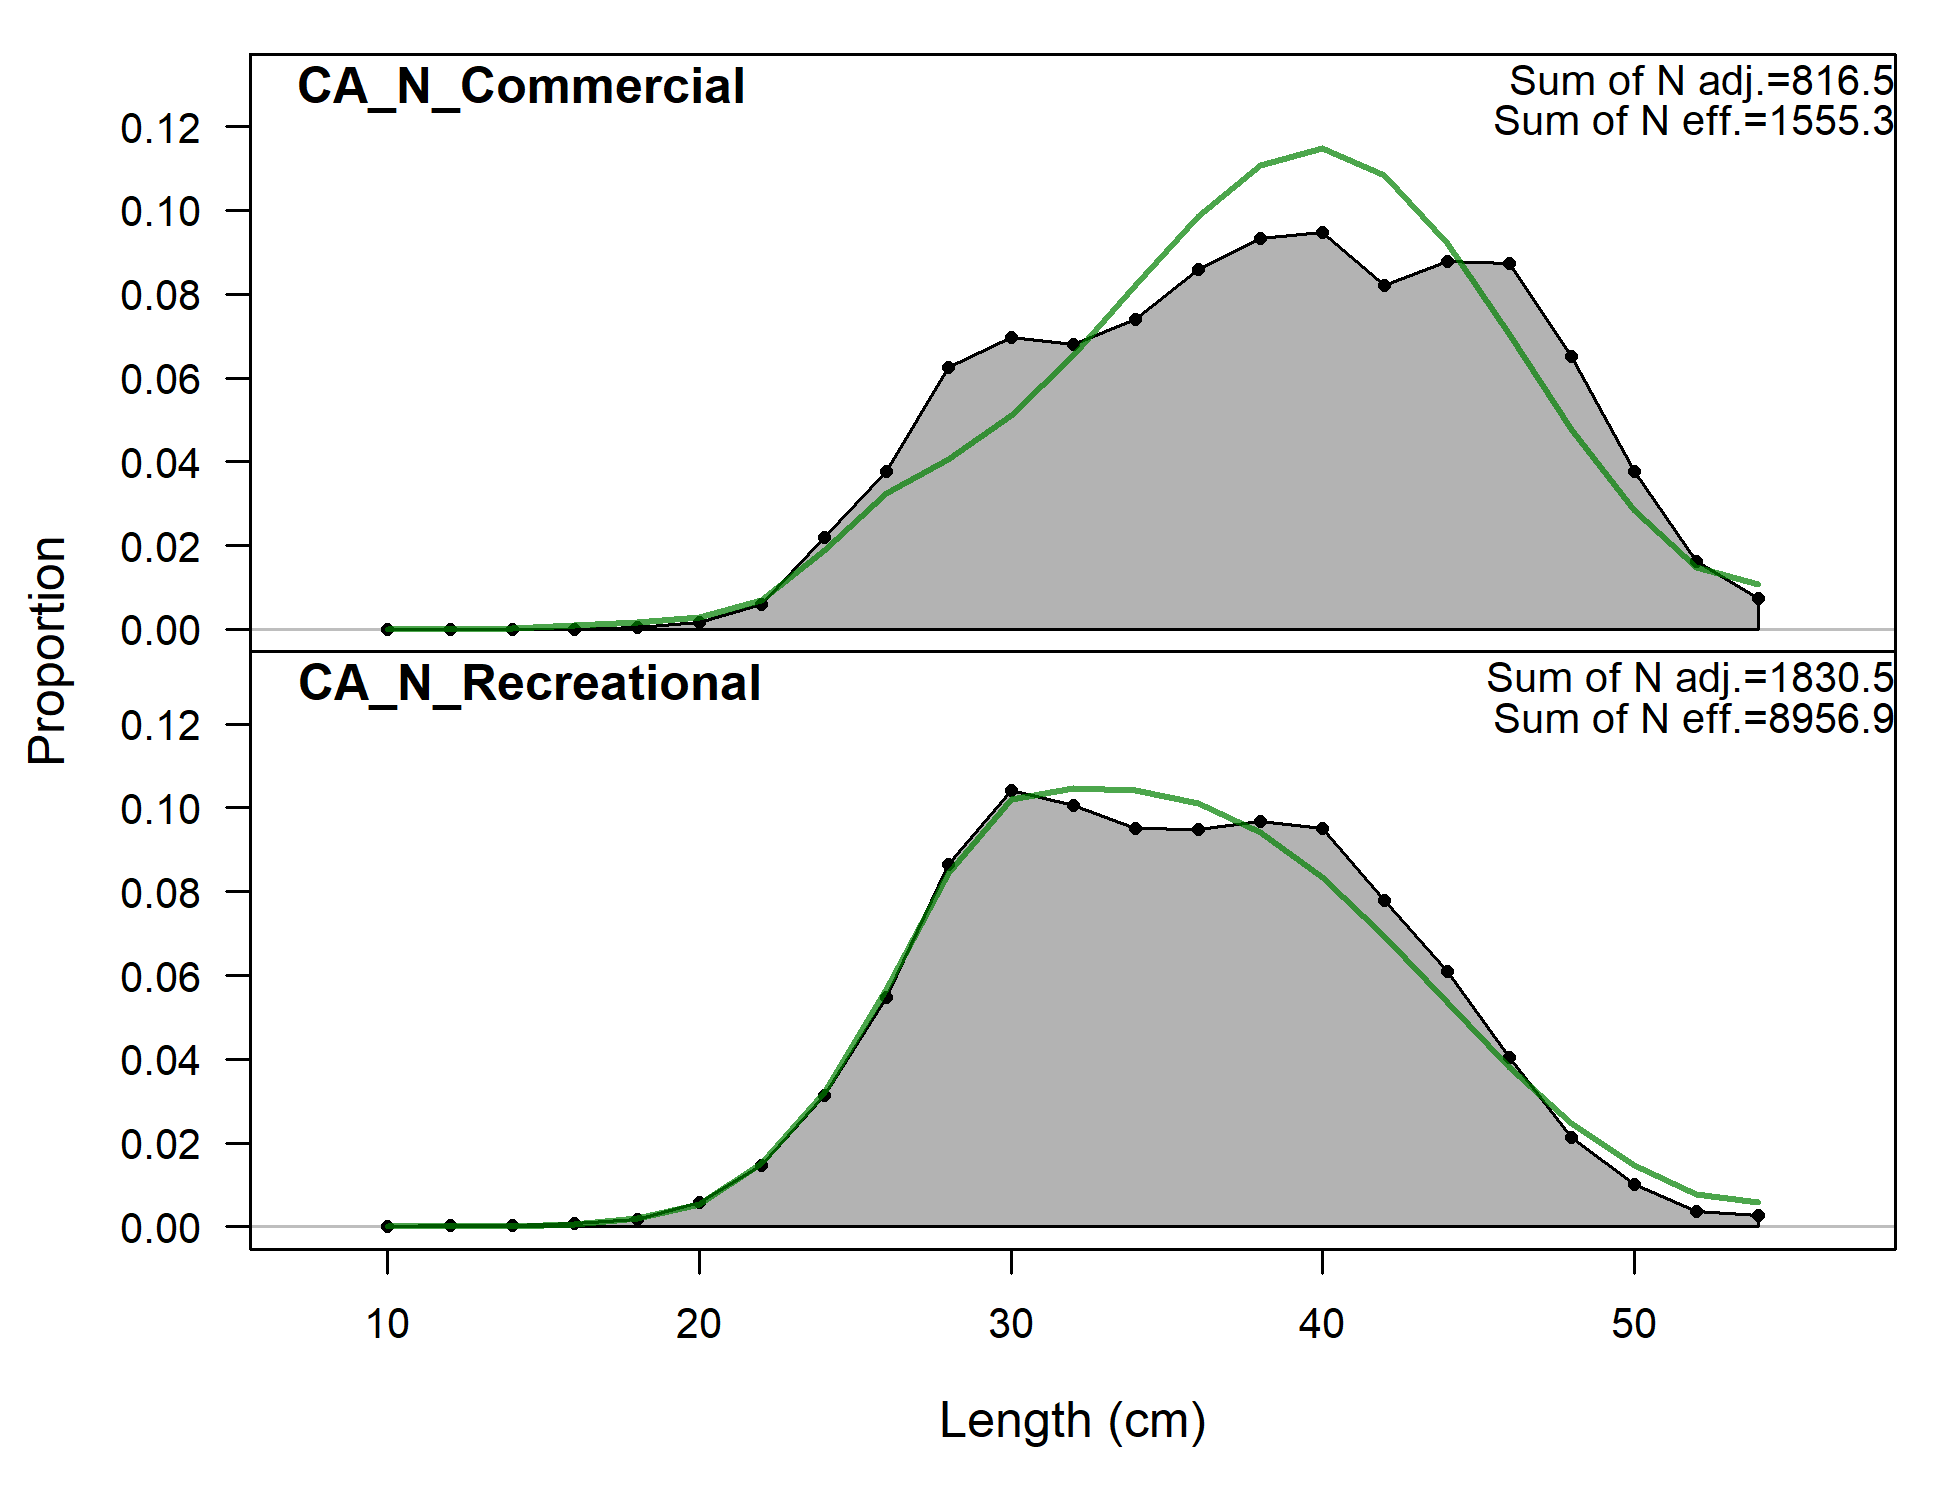
\includegraphics[width=1\textwidth,height=1\textheight]{C:/Assessments/2021/copper_rockfish_2021/models/ca_s_pt_c/12.1_base/plots/comp_lenfit__aggregated_across_time.png}
\caption{Aggregated length comps over all years.\label{fig:agg-len-fit}}
\end{figure}

\tagmcend\tagstructend

\tagstructbegin{tag=Figure,alttext={.}}\tagmcbegin{tag=Figure}

\begin{figure}
\centering
\includegraphics[width=1\textwidth,height=1\textheight]{C:/Assessments/2021/copper_rockfish_2021/models/ca_s_pt_c/12.1_base/plots/index2_cpuefit_NWFSC_HKL.png}
\caption{Fit to index data for the NWFSC Hook and Line survey.\label{fig:index-fit}}
\end{figure}

\tagmcend\tagstructend

\tagstructbegin{tag=Figure,alttext={.}}\tagmcbegin{tag=Figure}

\begin{figure}
\centering
\includegraphics[width=1\textwidth,height=1\textheight]{C:/Assessments/2021/copper_rockfish_2021/models/ca_s_pt_c/12.1_base/plots/ts7_Spawning_output_with_95_asymptotic_intervals_intervals.png}
\caption{Estimated time series of spawning output.\label{fig:ssb}}
\end{figure}

\tagmcend\tagstructend

\tagstructbegin{tag=Figure,alttext={.}}\tagmcbegin{tag=Figure}

\begin{figure}
\centering
\includegraphics[width=1\textwidth,height=1\textheight]{C:/Assessments/2021/copper_rockfish_2021/models/ca_s_pt_c/12.1_base/plots/ts1_Total_biomass_(mt).png}
\caption{Estimated time series of total biomass.\label{fig:tot-bio}}
\end{figure}

\tagmcend\tagstructend

\tagstructbegin{tag=Figure,alttext={.}}\tagmcbegin{tag=Figure}

\begin{figure}
\centering
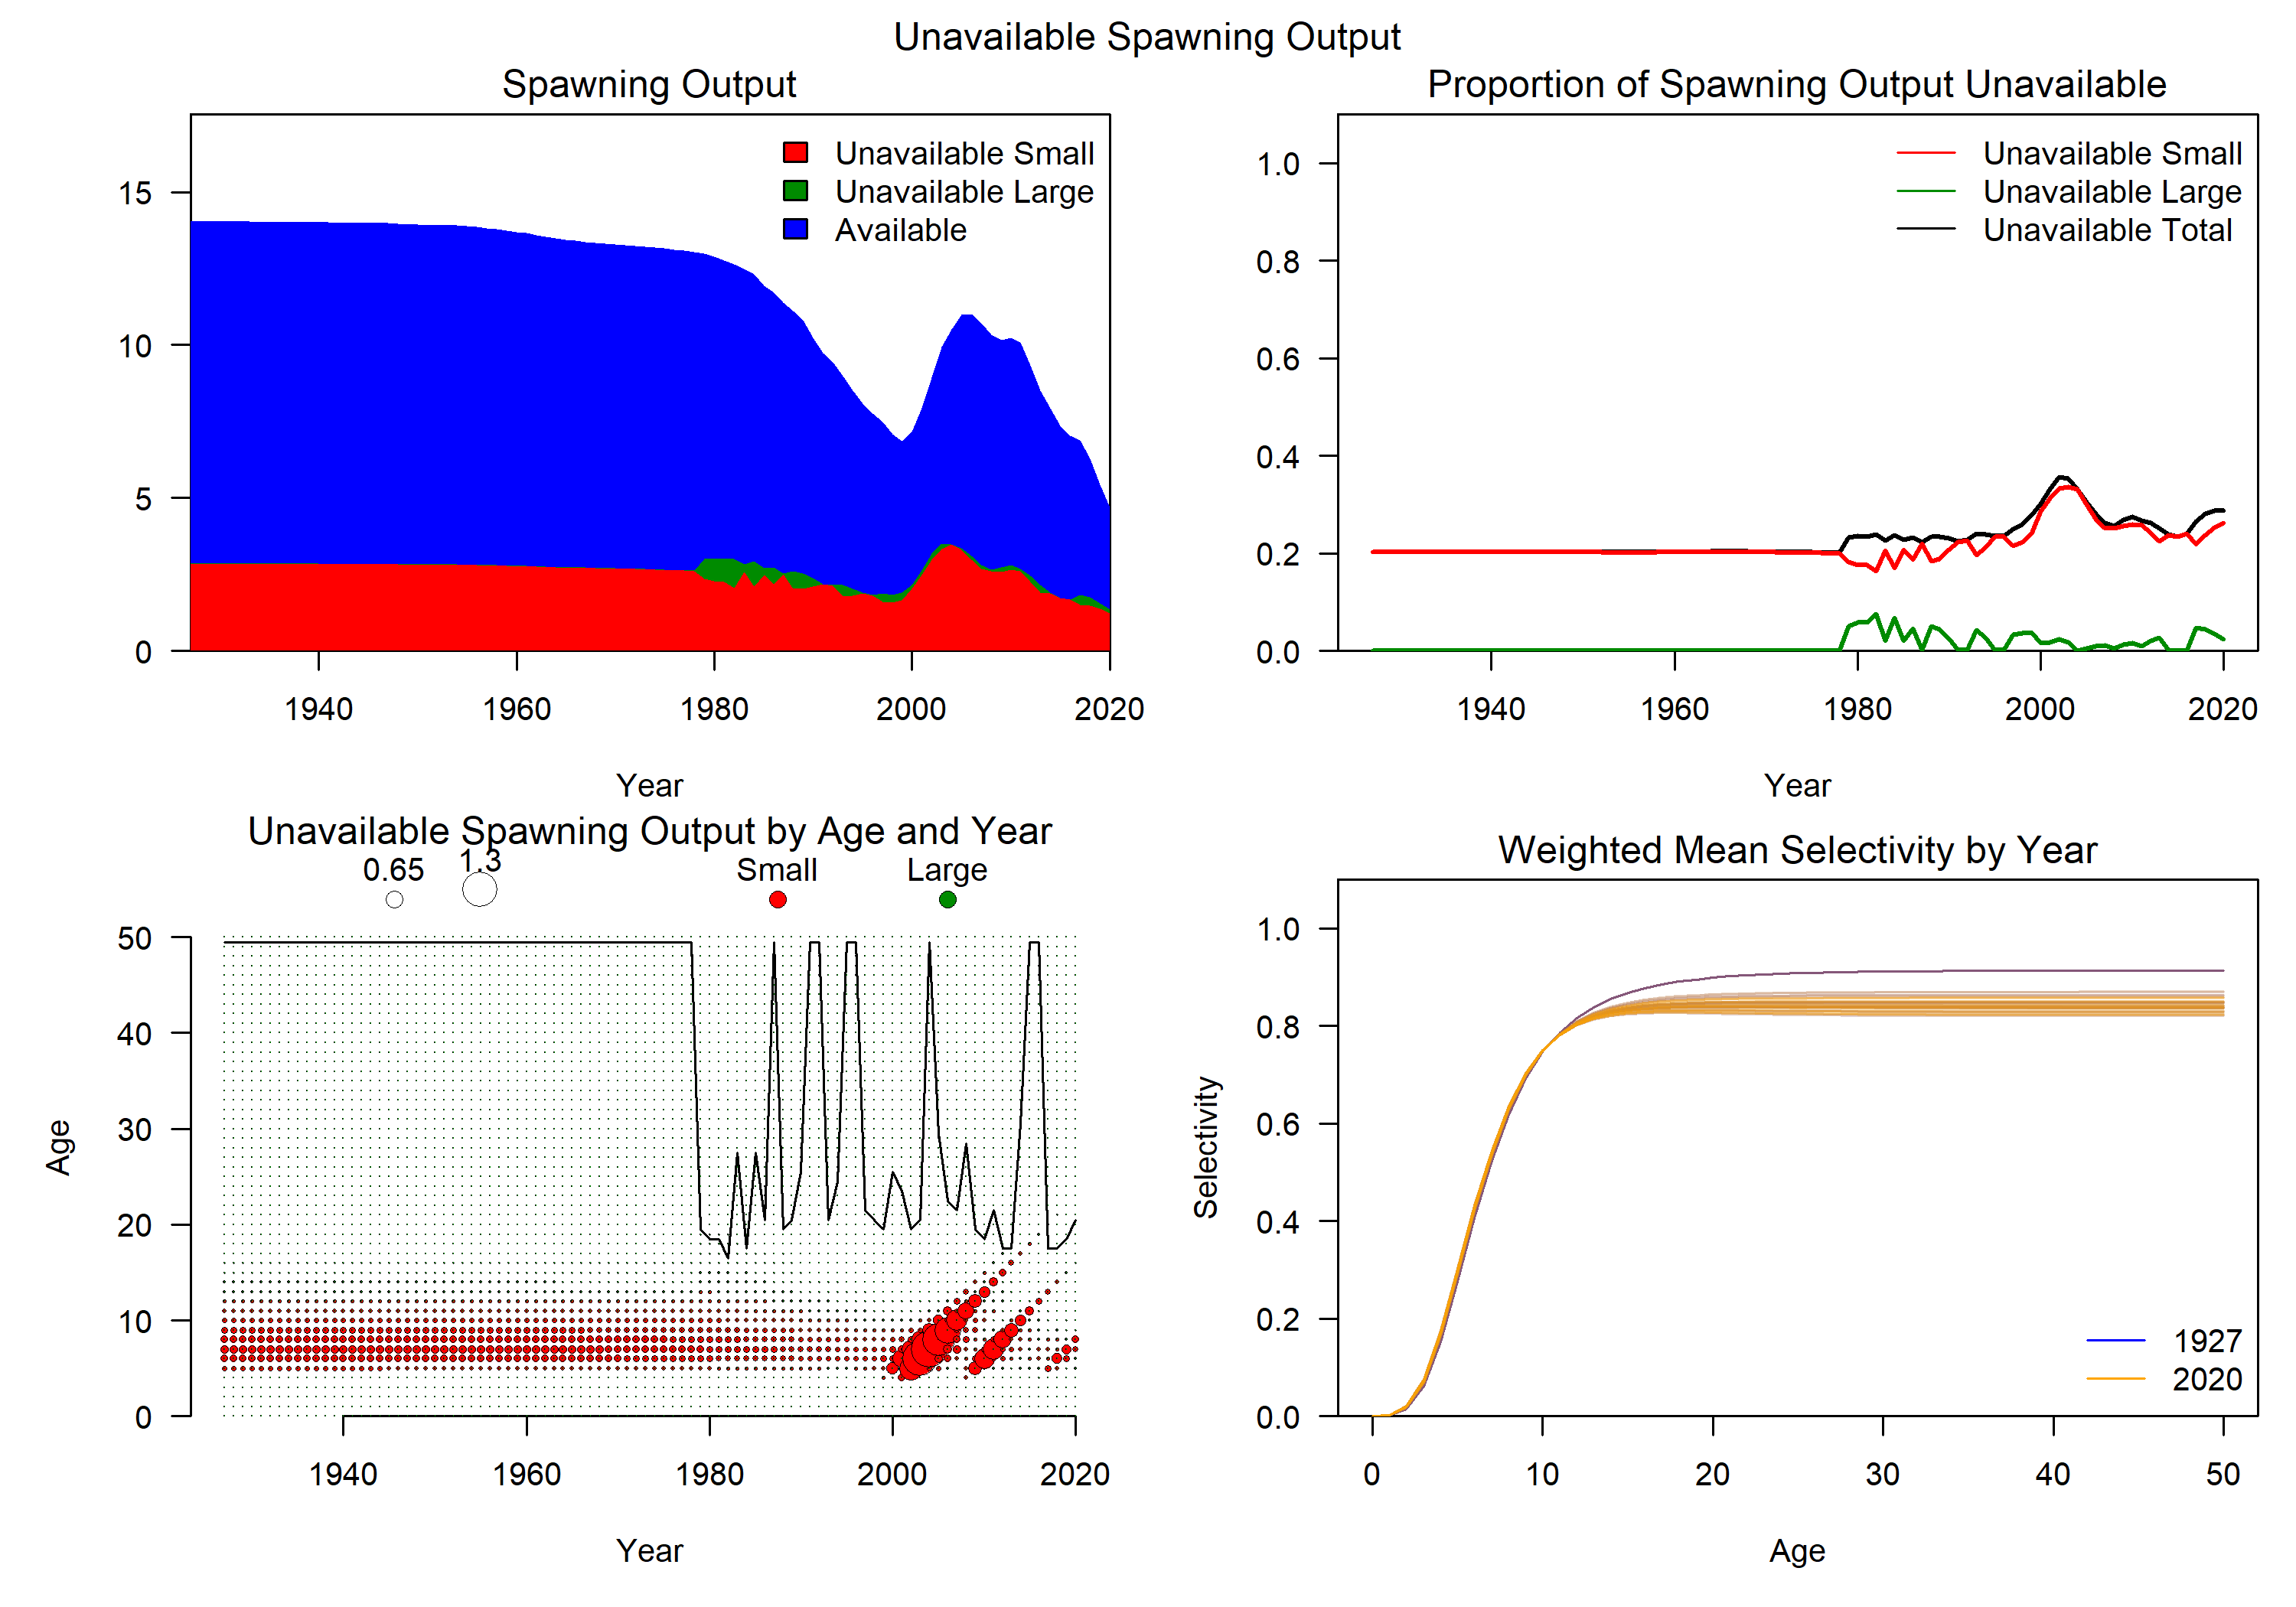
\includegraphics[width=1\textwidth,height=1\textheight]{C:/Assessments/2021/copper_rockfish_2021/write_up/s_ca/figs/unavailable_biomass.png}
\caption{Estimated time series of unavailable spawning output.\label{fig:ssb-unavailable}}
\end{figure}

\tagmcend\tagstructend

\tagstructbegin{tag=Figure,alttext={.}}\tagmcbegin{tag=Figure}

\begin{figure}
\centering
\includegraphics[width=1\textwidth,height=1\textheight]{C:/Assessments/2021/copper_rockfish_2021/models/ca_s_pt_c/12.1_base/plots/ts9_Fraction_of_unfished_with_95_asymptotic_intervals_intervals.png}
\caption{Estimated time series of fraction of unfished spawning output.\label{fig:depl}}
\end{figure}

\tagmcend\tagstructend

\tagstructbegin{tag=Figure,alttext={.}}\tagmcbegin{tag=Figure}

\begin{figure}
\centering
\includegraphics[width=1\textwidth,height=1\textheight]{//nwcfile/FRAM/Assessments/CurrentAssessments/DataModerate_2021/copper_rockfish/models/ca_s_pt_c/_sensitivities/_plots/12.1_base_final_1_compare2_spawnbio_uncertainty.png}
\caption{Change in estimated spawning output by sensitivity.\label{fig:sens-ssb-1}}
\end{figure}

\tagmcend\tagstructend

\tagstructbegin{tag=Figure,alttext={.}}\tagmcbegin{tag=Figure}

\begin{figure}
\centering
\includegraphics[width=1\textwidth,height=1\textheight]{//nwcfile/FRAM/Assessments/CurrentAssessments/DataModerate_2021/copper_rockfish/models/ca_s_pt_c/_sensitivities/_plots/12.1_base_final_1_compare4_Bratio_uncertainty.png}
\caption{Change in estimated fraction unfished by sensitivity.\label{fig:sens-depl-1}}
\end{figure}

\tagmcend\tagstructend

\tagstructbegin{tag=Figure,alttext={.}}\tagmcbegin{tag=Figure}

\begin{figure}
\centering
\includegraphics[width=1\textwidth,height=1\textheight]{//nwcfile/FRAM/Assessments/CurrentAssessments/DataModerate_2021/copper_rockfish/models/ca_s_pt_c/_sensitivities/_plots/12.1_base_final_2_compare2_spawnbio_uncertainty.png}
\caption{Change in estimated spawning output by sensitivity.\label{fig:sens-ssb-2}}
\end{figure}

\tagmcend\tagstructend

\tagstructbegin{tag=Figure,alttext={.}}\tagmcbegin{tag=Figure}

\begin{figure}
\centering
\includegraphics[width=1\textwidth,height=1\textheight]{//nwcfile/FRAM/Assessments/CurrentAssessments/DataModerate_2021/copper_rockfish/models/ca_s_pt_c/_sensitivities/_plots/12.1_base_final_2_compare4_Bratio_uncertainty.png}
\caption{Change in estimated fraction unfished by sensitivity.\label{fig:sens-depl-2}}
\end{figure}

\tagmcend\tagstructend

\newpage

\tagstructbegin{tag=Figure,alttext={.}}\tagmcbegin{tag=Figure}

\begin{figure}
\centering
\includegraphics[width=1\textwidth,height=1\textheight]{//nwcfile/FRAM/Assessments/CurrentAssessments/DataModerate_2021/copper_rockfish/models/ca_s_pt_c/_sensitivities/_plots/12.1_base_area_compare2_spawnbio_uncertainty.png}
\caption{Change in estimated spawning output by sensitivity examining alternative percent of the population protected from fishing.\label{fig:sens-area-ssb}}
\end{figure}

\tagmcend\tagstructend

\tagstructbegin{tag=Figure,alttext={.}}\tagmcbegin{tag=Figure}

\begin{figure}
\centering
\includegraphics[width=1\textwidth,height=1\textheight]{//nwcfile/FRAM/Assessments/CurrentAssessments/DataModerate_2021/copper_rockfish/models/ca_s_pt_c/_sensitivities/_plots/12.1_base_area_compare4_Bratio_uncertainty.png}
\caption{Change in estimated fraction unfished by sensitivity examining alternative percent of the population protected from fishing.\label{fig:sens-area-depl}}
\end{figure}

\tagmcend\tagstructend

\newpage

\tagstructbegin{tag=Figure,alttext={.}}\tagmcbegin{tag=Figure}

\begin{figure}
\centering
\includegraphics[width=1\textwidth,height=1\textheight]{C:/Assessments/2021/copper_rockfish_2021/models/ca_s_pt_c/12.1_base_profile_SR_LN(R0)/piner_panel_SR_LN(R0).png}
\caption{Change in the negative log-likelihood across a range of log(R0) values.\label{fig:r0-profile}}
\end{figure}

\tagmcend\tagstructend

\tagstructbegin{tag=Figure,alttext={.}}\tagmcbegin{tag=Figure}

\begin{figure}
\centering
\includegraphics[width=1\textwidth,height=1\textheight]{C:/Assessments/2021/copper_rockfish_2021/models/ca_s_pt_c/12.1_base_profile_SR_LN(R0)/SR_LN(R0)_trajectories_compare1_spawnbio.png}
\caption{Change in the estimate of spawning output across a range of log(R0) values.\label{fig:r0-ssb}}
\end{figure}

\tagmcend\tagstructend

\tagstructbegin{tag=Figure,alttext={.}}\tagmcbegin{tag=Figure}

\begin{figure}
\centering
\includegraphics[width=1\textwidth,height=1\textheight]{C:/Assessments/2021/copper_rockfish_2021/models/ca_s_pt_c/12.1_base_profile_SR_LN(R0)/SR_LN(R0)_trajectories_compare3_Bratio.png}
\caption{Change in the estimate of fraction unfished across a range of log(R0) values.\label{fig:r0-depl}}
\end{figure}

\tagmcend\tagstructend

\tagstructbegin{tag=Figure,alttext={.}}\tagmcbegin{tag=Figure}

\begin{figure}
\centering
\includegraphics[width=1\textwidth,height=1\textheight]{C:/Assessments/2021/copper_rockfish_2021/models/ca_s_pt_c/12.1_base_profile_SR_BH_steep/piner_panel_SR_BH_steep.png}
\caption{Change in the negative log-likelihood across a range of steepness values.\label{fig:h-profile}}
\end{figure}

\tagmcend\tagstructend

\tagstructbegin{tag=Figure,alttext={.}}\tagmcbegin{tag=Figure}

\begin{figure}
\centering
\includegraphics[width=1\textwidth,height=1\textheight]{C:/Assessments/2021/copper_rockfish_2021/models/ca_s_pt_c/12.1_base_profile_SR_BH_steep/SR_BH_steep_trajectories_compare1_spawnbio.png}
\caption{Change in the estimate of spawning output across a range of steepness values.\label{fig:h-ssb}}
\end{figure}

\tagmcend\tagstructend

\tagstructbegin{tag=Figure,alttext={.}}\tagmcbegin{tag=Figure}

\begin{figure}
\centering
\includegraphics[width=1\textwidth,height=1\textheight]{C:/Assessments/2021/copper_rockfish_2021/models/ca_s_pt_c/12.1_base_profile_SR_BH_steep/SR_BH_steep_trajectories_compare3_Bratio.png}
\caption{Change in the estimate of fraction unfished across a range of steepness values.\label{fig:h-depl}}
\end{figure}

\tagmcend\tagstructend

\tagstructbegin{tag=Figure,alttext={.}}\tagmcbegin{tag=Figure}

\begin{figure}
\centering
\includegraphics[width=1\textwidth,height=1\textheight]{C:/Assessments/2021/copper_rockfish_2021/models/ca_s_pt_c/12.1_base_profile_NatM_p_1_Fem_GP_1/piner_panel_NatM_p_1_Fem_GP_1.png}
\caption{Change in the negative log-likelihood across a range of female natural mortality values.\label{fig:m-profile}}
\end{figure}

\tagmcend\tagstructend

\tagstructbegin{tag=Figure,alttext={.}}\tagmcbegin{tag=Figure}

\begin{figure}
\centering
\includegraphics[width=1\textwidth,height=1\textheight]{C:/Assessments/2021/copper_rockfish_2021/models/ca_s_pt_c/12.1_base_profile_NatM_p_1_Fem_GP_1/NatM_p_1_Fem_GP_1_trajectories_compare1_spawnbio.png}
\caption{Change in the estimate of spawning output across a range of female natural mortality values.\label{fig:m-ssb}}
\end{figure}

\tagmcend\tagstructend

\tagstructbegin{tag=Figure,alttext={.}}\tagmcbegin{tag=Figure}

\begin{figure}
\centering
\includegraphics[width=1\textwidth,height=1\textheight]{C:/Assessments/2021/copper_rockfish_2021/models/ca_s_pt_c/12.1_base_profile_NatM_p_1_Fem_GP_1/NatM_p_1_Fem_GP_1_trajectories_compare3_Bratio.png}
\caption{Change in the estimate of fraction unfished across a range of female natural values.\label{fig:m-depl}}
\end{figure}

\tagmcend\tagstructend

\tagstructbegin{tag=Figure,alttext={.}}\tagmcbegin{tag=Figure}

\begin{figure}
\centering
\includegraphics[width=1\textwidth,height=1\textheight]{C:/Assessments/2021/copper_rockfish_2021/models/ca_s_pt_c/12.1_base_profile_L_at_Amax_Fem_GP_1/piner_panel_L_at_Amax_Fem_GP_1.png}
\caption{Change in the negative log-likelihood across a range of female maximum length values.\label{fig:linf-profile}}
\end{figure}

\tagmcend\tagstructend

\tagstructbegin{tag=Figure,alttext={.}}\tagmcbegin{tag=Figure}

\begin{figure}
\centering
\includegraphics[width=1\textwidth,height=1\textheight]{C:/Assessments/2021/copper_rockfish_2021/models/ca_s_pt_c/12.1_base_profile_L_at_Amax_Fem_GP_1/L_at_Amax_Fem_GP_1_trajectories_compare1_spawnbio.png}
\caption{Change in the estimate of spawning output across a range of female maximum length values.\label{fig:linf-ssb}}
\end{figure}

\tagmcend\tagstructend

\tagstructbegin{tag=Figure,alttext={.}}\tagmcbegin{tag=Figure}

\begin{figure}
\centering
\includegraphics[width=1\textwidth,height=1\textheight]{C:/Assessments/2021/copper_rockfish_2021/models/ca_s_pt_c/12.1_base_profile_L_at_Amax_Fem_GP_1/L_at_Amax_Fem_GP_1_trajectories_compare3_Bratio.png}
\caption{Change in the estimate of fraction unfished across a range of female maximum length values.\label{fig:linf-depl}}
\end{figure}

\tagmcend\tagstructend

\tagstructbegin{tag=Figure,alttext={.}}\tagmcbegin{tag=Figure}

\begin{figure}
\centering
\includegraphics[width=1\textwidth,height=1\textheight]{C:/Assessments/2021/copper_rockfish_2021/models/ca_s_pt_c/12.1_base_profile_VonBert_K_Fem_GP_1/piner_panel_VonBert_K_Fem_GP_1.png}
\caption{Change in the negative log-likelihood across a range of female k values.\label{fig:k-profile}}
\end{figure}

\tagmcend\tagstructend

\tagstructbegin{tag=Figure,alttext={.}}\tagmcbegin{tag=Figure}

\begin{figure}
\centering
\includegraphics[width=1\textwidth,height=1\textheight]{C:/Assessments/2021/copper_rockfish_2021/models/ca_s_pt_c/12.1_base_profile_VonBert_K_Fem_GP_1/VonBert_K_Fem_GP_1_trajectories_compare1_spawnbio.png}
\caption{Change in the estimate of spawning output across a range of female k values.\label{fig:k-ssb}}
\end{figure}

\tagmcend\tagstructend

\tagstructbegin{tag=Figure,alttext={.}}\tagmcbegin{tag=Figure}

\begin{figure}
\centering
\includegraphics[width=1\textwidth,height=1\textheight]{C:/Assessments/2021/copper_rockfish_2021/models/ca_s_pt_c/12.1_base_profile_VonBert_K_Fem_GP_1/VonBert_K_Fem_GP_1_trajectories_compare3_Bratio.png}
\caption{Change in the estimate of fraction unfished across a range of female k values.\label{fig:k-depl}}
\end{figure}

\tagmcend\tagstructend

\tagstructbegin{tag=Figure,alttext={.}}\tagmcbegin{tag=Figure}

\begin{figure}
\centering
\includegraphics[width=1\textwidth,height=1\textheight]{C:/Assessments/2021/copper_rockfish_2021/models/ca_s_pt_c/12.1_base_profile_CV_old_Fem_GP_1/piner_panel_CV_old_Fem_GP_1.png}
\caption{Change in the negative log-likelihood across a range of female coefficient of variation for older ages.\label{fig:cv-profile}}
\end{figure}

\tagmcend\tagstructend

\tagstructbegin{tag=Figure,alttext={.}}\tagmcbegin{tag=Figure}

\begin{figure}
\centering
\includegraphics[width=1\textwidth,height=1\textheight]{C:/Assessments/2021/copper_rockfish_2021/models/ca_s_pt_c/12.1_base_profile_CV_old_Fem_GP_1/CV_old_Fem_GP_1_trajectories_compare1_spawnbio.png}
\caption{Change in the estimate of spawning output across a range of female coefficient of variation for older ages.\label{fig:cv-ssb}}
\end{figure}

\tagmcend\tagstructend

\tagstructbegin{tag=Figure,alttext={.}}\tagmcbegin{tag=Figure}

\begin{figure}
\centering
\includegraphics[width=1\textwidth,height=1\textheight]{C:/Assessments/2021/copper_rockfish_2021/models/ca_s_pt_c/12.1_base_profile_CV_old_Fem_GP_1/CV_old_Fem_GP_1_trajectories_compare3_Bratio.png}
\caption{Change in the estimate of fraction unfished across a range of female coefficient of variation for older ages.\label{fig:cv-depl}}
\end{figure}

\tagmcend\tagstructend

\clearpage

\tagstructbegin{tag=Figure,alttext={.}}\tagmcbegin{tag=Figure}

\begin{figure}
\centering
\includegraphics[width=1\textwidth,height=1\textheight]{C:/Assessments/2021/copper_rockfish_2021/models/lbspr/Copper_SoCAL_YrEsts_newVBGF.png}
\caption{LB-SPR yearly estimates of selectivity, the ratio of fishing intensity to natural mortality (F/M), and annual spawner-per-recruit (SPR) values.\label{fig:lbspr}}
\end{figure}

\tagmcend\tagstructend

\newpage

\tagstructbegin{tag=Figure,alttext={.}}\tagmcbegin{tag=Figure}

\begin{figure}
\centering
\includegraphics[width=1\textwidth,height=1\textheight]{C:/Assessments/2021/copper_rockfish_2021/models/ca_s_pt_c/12.1_base_retro/compare2_spawnbio_uncertainty.png}
\caption{Change in the estimate of spawning output when the most recent 10 years of data area removed sequentially.\label{fig:retro-ssb}}
\end{figure}

\tagmcend\tagstructend

\tagstructbegin{tag=Figure,alttext={.}}\tagmcbegin{tag=Figure}

\begin{figure}
\centering
\includegraphics[width=1\textwidth,height=1\textheight]{C:/Assessments/2021/copper_rockfish_2021/models/ca_s_pt_c/12.1_base_retro/compare4_Bratio_uncertainty.png}
\caption{Change in the estimate of fraction unfished when the most recent 10 years of data area removed sequentially.\label{fig:retro-depl}}
\end{figure}

\tagmcend\tagstructend

\newpage

\tagstructbegin{tag=Figure,alttext={.}}\tagmcbegin{tag=Figure}

\begin{figure}
\centering
\includegraphics[width=1\textwidth,height=1\textheight]{//nwcfile/FRAM/Assessments/CurrentAssessments/DataModerate_2021/copper_rockfish/models/_plots/ca_comprare_compare2_spawnbio_uncertainty.png}
\caption{Estimated spawning output time series for the California stocks north and south of Point Conception.\label{fig:ssb-ca-compare}}
\end{figure}

\tagmcend\tagstructend

\tagstructbegin{tag=Figure,alttext={.}}\tagmcbegin{tag=Figure}

\begin{figure}
\centering
\includegraphics[width=1\textwidth,height=1\textheight]{//nwcfile/FRAM/Assessments/CurrentAssessments/DataModerate_2021/copper_rockfish/models/_plots/or_wa_comprare_compare2_spawnbio_uncertainty.png}
\caption{Estimated spawning output time series for the stocks off the Oregon and Washington coast.\label{fig:ssb-orwa-compare}}
\end{figure}

\tagmcend\tagstructend

\tagstructbegin{tag=Figure,alttext={.}}\tagmcbegin{tag=Figure}

\begin{figure}
\centering
\includegraphics[width=1\textwidth,height=1\textheight]{//nwcfile/FRAM/Assessments/CurrentAssessments/DataModerate_2021/copper_rockfish/models/_plots/comprare_compare4_Bratio_uncertainty.png}
\caption{Estimated fraction unfished time series for all West Coast stocks.\label{fig:depl-compare}}
\end{figure}

\tagmcend\tagstructend

\clearpage

\tagstructbegin{tag=Figure,alttext={.}}\tagmcbegin{tag=Figure}

\begin{figure}
\centering
\includegraphics[width=1\textwidth,height=1\textheight]{C:/Assessments/2021/copper_rockfish_2021/write_up/s_ca/figs/assess_compare_compare2_spawnbio_uncertainty.png}
\caption{The estimated spawning output from the base model and the 2013 assessment. The 2013 model estimated spawning biomass (mt) and the 2021 assessment is terms of spawning output (millions of eggs).\label{fig:compare-ssb-2013}}
\end{figure}

\tagmcend\tagstructend

\tagstructbegin{tag=Figure,alttext={.}}\tagmcbegin{tag=Figure}

\begin{figure}
\centering
\includegraphics[width=1\textwidth,height=1\textheight]{C:/Assessments/2021/copper_rockfish_2021/write_up/s_ca/figs/assess_compare_compare4_Bratio_uncertainty.png}
\caption{The estimated fraction unfished from the base model and the 2013 assessment.\label{fig:compare-depl-2013}}
\end{figure}

\tagmcend\tagstructend

\newpage

\tagstructbegin{tag=Figure,alttext={.}}\tagmcbegin{tag=Figure}

\begin{figure}
\centering
\includegraphics[width=1\textwidth,height=1\textheight]{C:/Assessments/2021/copper_rockfish_2021/models/ca_s_pt_c/12.1_base/plots/SPR2_minusSPRseries.png}
\caption{Estimated 1 - relative spawning ratio (SPR) by year.\label{fig:1-spr}}
\end{figure}

\tagmcend\tagstructend

\tagstructbegin{tag=Figure,alttext={.}}\tagmcbegin{tag=Figure}

\begin{figure}
\centering
\includegraphics[width=1\textwidth,height=1\textheight]{C:/Assessments/2021/copper_rockfish_2021/models/ca_s_pt_c/12.1_base/plots/SPR4_phase.png}
\caption{Phase plot of the relative biomass (also referred to as fraction unfished) versus the SPR ratio where each point represents the biomass ratio at the start of the year and the relative fishing intensity in that same year. Lines through the final point show the 95 percent intervals based on the asymptotic uncertainty for each dimension. The shaded ellipse is a 95 percent region which accounts for the estimated correlations between the biomass ratio and SPR ratio.\label{fig:phase}}
\end{figure}

\tagmcend\tagstructend

\tagstructbegin{tag=Figure,alttext={.}}\tagmcbegin{tag=Figure}

\begin{figure}
\centering
\includegraphics[width=1\textwidth,height=1\textheight]{C:/Assessments/2021/copper_rockfish_2021/models/ca_s_pt_c/12.1_base/plots/yield2_yield_curve_with_refpoints.png}
\caption{Equilibrium yield curve for the base case model. Values are based on the 2020 fishery selectivity and with steepness fixed at 0.72.\label{fig:yield}}
\end{figure}

\tagmcend\tagstructend

\clearpage

\tagstructbegin{tag=H1}\tagmcbegin{tag=H1}

\hypertarget{appendix}{%
\section{Appendix}\label{appendix}}

\leavevmode\tagmcend\tagstructend

\tagstructbegin{tag=H2}\tagmcbegin{tag=H2}

\hypertarget{ca-man}{%
\subsection{Summary of California Management Measures}\label{ca-man}}

\leavevmode\tagmcend\tagstructend

\tagstructbegin{tag=P}\tagmcbegin{tag=P}

Information on changes to California management measures across time can be found in the separate file ``California Nearshore Regulation History-Data Moderate Accompanying Material.pdf''.

\leavevmode\tagmcend\tagstructend\par

\tagstructbegin{tag=H2}\tagmcbegin{tag=H2}

\hypertarget{ca-closed-open}{%
\subsection{Percent of Habitat Area Closed to Fishing for Groundfish in the Rockfish Conservation Areas, Cowcod Conservation Areas, and Marine Protected Areas in California from 2001-2021}\label{ca-closed-open}}

\leavevmode\tagmcend\tagstructend

\tagstructbegin{tag=P}\tagmcbegin{tag=P}

At present, stock assessments reliant on fishery dependent data only represent the areas open to fishing, unless there is a fishery independent data source providing information on the relative abundance and length composition in closed areas. A network of marine protected areas (MPAs) was established between 2003 to 2012 through a regional siting process. The length composition and relative abundance inside and outside MPAs in part results from the presence of MPAs prohibiting take of groundfish established prior to expansion of the current network, duration of existence of new areas, degree of effort prior to protection and criteria for selection focusing on high productivity reefs. These areas are established in perpetuity and will provide substantial protections to nearshore fish stocks for the foreseeable future.

\leavevmode\tagmcend\tagstructend\par

\tagstructbegin{tag=P}\tagmcbegin{tag=P}

In addition to MPAs, extensive Rockfish Conservation Areas (RCAs) of varying depths over time and space, as well as the two cowcod conservation areas (CCAs) encompassing 4200 square miles of water area since 2001, were established to facilitate rebuilding of overfished species. While the depth restrictions in these closed areas can change or be eliminated, the areas closed become refugia that reduce fishing mortality, allowing accumulation of biomass within them. There has long been interest in quantifying the area of reef habitat for each assessed species that resides in protected areas, but until very recently, there was insufficient data on the distribution of rocky reef habitat. This analysis provides the percentage of habitat area for copper and quillback rockfish closed to fishing in MPAs, RCAs and CCAs where the take of groundfish was prohibited in each year from 2001 to 2021.

\leavevmode\tagmcend\tagstructend\par

\tagstructbegin{tag=H3}\tagmcbegin{tag=H3}

\hypertarget{methods}{%
\subsubsection{Methods}\label{methods}}

\leavevmode\tagmcend\tagstructend

\tagstructbegin{tag=H4}\tagmcbegin{tag=H4}

\hypertarget{descriptions-of-the-habitat-layers}{%
\paragraph{Descriptions of the habitat layers}\label{descriptions-of-the-habitat-layers}}

\leavevmode\tagmcend\tagstructend

\tagstructbegin{tag=P}\tagmcbegin{tag=P}

A predictive substrate layer that identifies hard and soft substrate was used to analyze seafloor coverage within the 3 nautical miles from California's shore. Substrate types were generated algorithmically using rugosity analysis, to identify areas likely to have rocky reefs. This layer was derived from bathymetric data of 2, 5 and 10 m resolution and bathymetric data were collected by California Seafloor Mapping Project (CSMP). Potential issues with this rugosity analysis include noise and artifacts resulting from unusual substrate structure, original mapping data, and steep slopes. In addition, hard substrate might be underestimated in areas with canyon slopes, deep water, over smooth rock and where sediments cover rock.

\leavevmode\tagmcend\tagstructend\par

\tagstructbegin{tag=P}\tagmcbegin{tag=P}

Data from the CSMP is known to have nearshore data gaps referred to as the white zone. Contributors from The University of California Santa Cruz, California Ocean Science Trust, and California Department of Fish and Wildlife (CDFW) conducted a 30 m resolution interpolation analysis to estimate hard and soft substrate within the white zone. The interpolation analysis utilized data from the CSMP and National Oceanic and the National Oceanic and Atmospheric Administration Environmental Sensitivity Index (ESI). Accuracy of the interpolation is estimated to be best where the white zone bands are narrowest and worst where the white zone bands are widest. In addition, metadata indicates the interpolation is questionable at scales finer than 100 m.

\leavevmode\tagmcend\tagstructend\par

\tagstructbegin{tag=P}\tagmcbegin{tag=P}

Substrate data developed for an Essential Fish Habitat Review was incorporated into this analysis for seafloor occurring outside of California State Waters (3 nautical miles). This dataset was generated by Joe Bizarro of the National Marine Fisheries Service, Southwest Fisheries Science Center in Santa Cruz and was created by combining multiple sources of bathymetric data with varying resolutions including multibeam sonar, sidescan sonar, sediment grabs, core samples seismic reflection profiles, still photos and video. This habitat data is subject to georeferencing errors and data resolution errors. Currently this is the best available data that represents hard and soft substrate types offshore for the areas outside of California State waters.

\leavevmode\tagmcend\tagstructend\par

\tagstructbegin{tag=H4}\tagmcbegin{tag=H4}

\hypertarget{boundaries-of-the-ccas-rcas-and-mpas}{%
\paragraph{Boundaries of the CCAs, RCAs and MPAs}\label{boundaries-of-the-ccas-rcas-and-mpas}}

\leavevmode\tagmcend\tagstructend

\tagstructbegin{tag=P}\tagmcbegin{tag=P}

Regulation histories for each type of closure were converted to Boolean fields with zeros and ones indicating absence and implementation, respectively from 2001-2020. The corresponding GIS layers were either available from previous CDFW GIS staff projects or approximated by the depth contour where specific weigh points were unavailable. The area in MPAs prohibiting take by the recreational and commercial fisheries were included in the estimates of area closed to fishing from the first year in which the MPA was in place for a full calendar year. The Western CCA area accounted for waters around islands and banks open to take of a limited suite of groundfish species including copper rockfish. The RCAs for commercial and recreational fisheries were based on the deeper of the depth restrictions for the sectors to reflect only areas where take was prohibited for both. Where the RCA lines for the stock in question were not available, depth contours were used to approximate the percent of area closed.

\leavevmode\tagmcend\tagstructend\par

\tagstructbegin{tag=H4}\tagmcbegin{tag=H4}

\hypertarget{delineating-habitat-in-restricted-areas-and-open-to-fishing}{%
\paragraph{Delineating Habitat in Restricted Areas and Open to Fishing}\label{delineating-habitat-in-restricted-areas-and-open-to-fishing}}

\leavevmode\tagmcend\tagstructend

\tagstructbegin{tag=P}\tagmcbegin{tag=P}

The depth range of habitat for copper and quillback rockfish was between shore to 100 m, covering the primary depth distribution of both stocks observed in the CDFW ROV survey (Budrick, Ryley and Prall 2020) or noted in Love et al.~(2002). The latitudinal range was set from the California/Mexican border to the California/Oregon border (42{\tagstructbegin{tag=Formula}\tagmcbegin{tag=Formula}\(^\circ\)\leavevmode\tagmcend\tagstructend} N. lat.), which was stratified north and south Point Conception (34{\tagstructbegin{tag=Formula}\tagmcbegin{tag=Formula}\(^\circ\)\leavevmode\tagmcend\tagstructend} 27' N. lat.). Quillback rockfish are relatively rare south of Point Conception, thus only estimates for the area north of Point Conception are pertinent to this stock, while copper rockfish are found in both areas.

\leavevmode\tagmcend\tagstructend\par

\tagstructbegin{tag=P}\tagmcbegin{tag=P}

The distribution and area of rocky reef habitat within a species range was delineated in ArcGIS Pro (2.6) by extracting specific values from a 10 m bathymetric raster based on species depth and latitudinal ranges. The resulting raster layer was converted into a shapefile and merged with a coastal boundary of California to account for gaps in the bathymetric raster. Hard habitat within the species range was identified and isolated using the intersect tool to create species range shapefile. This process was repeated to identify overlapping coverage between the species range and hard substrate, as well as intersecting the species range with a combination of different types of regulatory boundaries.

\leavevmode\tagmcend\tagstructend\par

\tagstructbegin{tag=P}\tagmcbegin{tag=P}

The area of the resulting shapefiles were calculated in GIS and exported into tables using Python script. The combination of area closures in a given year were overlayed on the habitat maps, with the area in MPAs and CCAs extracted first, then the habitat in the remaining RCAs estimated. The residual habitat still open to fishing after accounting for the closed areas was then estimated. The area of rocky reef habitat closed to fishing within a species range was converted to a percentage of the total habitat. This process for identifying overlapping boundaries and calculating areas were scripted in Python to reduce the possibility of human error.

\leavevmode\tagmcend\tagstructend\par

\tagstructbegin{tag=H4}\tagmcbegin{tag=H4}

\hypertarget{examination-of-bottom-type-coverage-relative-to-habitat}{%
\paragraph{Examination of bottom type coverage relative to habitat}\label{examination-of-bottom-type-coverage-relative-to-habitat}}

\leavevmode\tagmcend\tagstructend

\tagstructbegin{tag=P}\tagmcbegin{tag=P}

The extent of existing substrate data within a given species range was examined through geospatial analysis. This included hard, soft, and unknown substrate for data from California Seafloor Mapping Project, and hard, mixed, and soft data from the EFH project. Both datasets were merged within the species range for copper and quillback rockfish. The resulting combination of substrate data was erased from the species range.

\leavevmode\tagmcend\tagstructend\par

\tagstructbegin{tag=H3}\tagmcbegin{tag=H3}

\hypertarget{results}{%
\subsubsection{Results}\label{results}}

\leavevmode\tagmcend\tagstructend

\tagstructbegin{tag=P}\tagmcbegin{tag=P}

The tables reflecting the percent of habitat area in RCAs, MPAs, CCAs closed to fishing for groundfish and waters open to fishing are provided for north of Point Conception (Table \ref{tab:north-ca-percent}) and south of Point Conception (Table \ref{tab:south-ca-percent}). The potential habitat within the depth primary depth range of the species, rocky reef habitat within the potential habitat, MPAs and CCAs are depicted for the entire state (Figure \ref{fig:ca-all-app}) and various regions along the state in Figures \ref{fig:north-ca-app} - \ref{fig:south-ca-app}.

\leavevmode\tagmcend\tagstructend\par

\tagstructbegin{tag=P}\tagmcbegin{tag=P}

We found minimal voids in coverage in habitat layers across the species range, with 0.13 square miles missing north of Point Conception and 4.95 square miles missing from the south of Point Conception.

\leavevmode\tagmcend\tagstructend\par

\tagstructbegin{tag=H3}\tagmcbegin{tag=H3}

\hypertarget{discussion}{%
\subsubsection{Discussion}\label{discussion}}

\leavevmode\tagmcend\tagstructend

\tagstructbegin{tag=P}\tagmcbegin{tag=P}

Current assessments do not account for length/age composition and differing fishing mortality rates inside and outside MPAs or waters in long-established CCAs and RCAs. As biomass accrues inside these areas, accounting for protections through area-based assessment methods or effects on selectivity should be considered as fishery dependent data will only reflect the length composition and density outside. There is the potential for future assessments to account for differences in length composition, fishing mortality and relative abundance in a two-area model in Stock Synthesis with available data from long-term MPA monitoring.

\leavevmode\tagmcend\tagstructend\par

\tagstructbegin{tag=P}\tagmcbegin{tag=P}

Additional high resolution side scan sonar data in waters seaward of the CSMP coverage would improve coverage and resolution of habitat data. Similar analyses for each nearshore or shallower distributed shelf rockfish species (i.e., vermilion rockfish) would be a helpful addition to stock assessments to inform time blocking and selectivity considerations. The extent and design of the network to function in this way is unique to California and it's efforts to conserve nearshore stocks. Until the closed areas can be accounted for explicitly in stock assessments, the substantial areas in MPAs should be taken into consideration as a buffer against overfishing, since they were established in the interest of preserving spawning stock to seed areas outside and other MPAs in the network.

\leavevmode\tagmcend\tagstructend\par

\newpage

\begingroup\fontsize{10}{12}\selectfont
\begingroup\fontsize{10}{12}\selectfont

\begin{longtable}[t]{l>{\raggedright\arraybackslash}p{2cm}>{\raggedright\arraybackslash}p{2cm}>{\raggedright\arraybackslash}p{2cm}}
\caption{\label{tab:north-ca-percent}Percent of rocky reef habitat within 100 meters in MPAs, RCAs closed to fishing for groundfish and waters open to fishing in California north of Point Conception}\\
\toprule
Year & Percent Protected by MPA & Percent Protected by RCA & Percent Open to Fishing\\
\midrule
\endfirsthead
\caption[]{\label{tab:north-ca-percent}Percent of rocky reef habitat within 100 meters in MPAs, RCAs closed to fishing for groundfish and waters open to fishing in California north of Point Conception \textit{(continued)}}\\
\toprule
Year & Percent Protected by MPA & Percent Protected by RCA & Percent Open to Fishing\\
\midrule
\endhead

\endfoot
\bottomrule
\endlastfoot
2001 & 0.03 & 0.00 & 0.97\\
2002 & 0.03 & 0.00 & 0.97\\
2003 & 0.03 & 0.41 & 0.55\\
2004 & 0.03 & 0.23 & 0.73\\
2005 & 0.03 & 0.30 & 0.67\\
2006 & 0.03 & 0.30 & 0.67\\
2007 & 0.03 & 0.28 & 0.69\\
2008 & 0.11 & 0.27 & 0.62\\
2009 & 0.11 & 0.27 & 0.62\\
2010 & 0.11 & 0.33 & 0.56\\
2011 & 0.17 & 0.29 & 0.54\\
2012 & 0.17 & 0.29 & 0.54\\
2013 & 0.20 & 0.27 & 0.53\\
2014 & 0.20 & 0.27 & 0.53\\
2015 & 0.20 & 0.24 & 0.56\\
2016 & 0.20 & 0.24 & 0.56\\
2017 & 0.20 & 0.14 & 0.66\\
2018 & 0.20 & 0.14 & 0.66\\
2019 & 0.20 & 0.11 & 0.68\\
2020 & 0.20 & 0.13 & 0.67\\
2021 & 0.20 & 0.05 & 0.75\\*
\end{longtable}
\endgroup{}
\endgroup{}

\begingroup\fontsize{10}{12}\selectfont
\begingroup\fontsize{10}{12}\selectfont

\begin{longtable}[t]{l>{\raggedright\arraybackslash}p{2.2cm}>{\raggedright\arraybackslash}p{2.2cm}>{\raggedright\arraybackslash}p{2.2cm}>{\raggedright\arraybackslash}p{2.2cm}}
\caption{\label{tab:south-ca-percent}Percent of rocky reef habitat within 100 meters in MPAs, RCAs, CCAs closed to fishing for groundfish and waters open to fishing in California south of Point Conception}\\
\toprule
Year & Percent Protected by MPA & Percent Protected by RCA & Percent Protected by CCA & Percent Open to Fishing\\
\midrule
\endfirsthead
\caption[]{\label{tab:south-ca-percent}Percent of rocky reef habitat within 100 meters in MPAs, RCAs, CCAs closed to fishing for groundfish and waters open to fishing in California south of Point Conception \textit{(continued)}}\\
\toprule
Year & Percent Protected by MPA & Percent Protected by RCA & Percent Protected by CCA & Percent Open to Fishing\\
\midrule
\endhead

\endfoot
\bottomrule
\endlastfoot
2001 & 0.01 & 0.00 & 0.34 & 0.65\\
2002 & 0.01 & 0.00 & 0.34 & 0.65\\
2003 & 0.01 & 0.16 & 0.34 & 0.49\\
2004 & 0.04 & 0.10 & 0.34 & 0.52\\
2005 & 0.04 & 0.10 & 0.34 & 0.52\\
2006 & 0.04 & 0.10 & 0.34 & 0.52\\
2007 & 0.04 & 0.10 & 0.34 & 0.52\\
2008 & 0.04 & 0.10 & 0.34 & 0.52\\
2009 & 0.04 & 0.10 & 0.34 & 0.52\\
2010 & 0.04 & 0.10 & 0.34 & 0.52\\
2011 & 0.04 & 0.10 & 0.34 & 0.52\\
2012 & 0.08 & 0.10 & 0.34 & 0.48\\
2013 & 0.08 & 0.10 & 0.34 & 0.48\\
2014 & 0.08 & 0.10 & 0.34 & 0.48\\
2015 & 0.08 & 0.10 & 0.34 & 0.48\\
2016 & 0.08 & 0.10 & 0.34 & 0.48\\
2017 & 0.08 & 0.10 & 0.34 & 0.48\\
2018 & 0.08 & 0.10 & 0.34 & 0.48\\
2019 & 0.08 & 0.10 & 0.25 & 0.57\\
2020 & 0.08 & 0.10 & 0.25 & 0.57\\
2021 & 0.08 & 0.10 & 0.25 & 0.57\\*
\end{longtable}
\endgroup{}
\endgroup{}

\tagstructbegin{tag=Figure,alttext={.}}\tagmcbegin{tag=Figure}

\begin{figure}
\centering
\includegraphics[width=1\textwidth,height=1\textheight]{//nwcfile/FRAM/Assessments/CurrentAssessments/DataModerate_2021/copper_rockfish/write_up/ca_appendix/ca_substrate.png}
\caption{Copper and quillback rockfish potential depth range off California in red hatched polygon, hard substrate occurring within the potential range in pink, MPAs in dark blue outline, and the CCAs in light blue.\label{fig:ca-all-app}}
\end{figure}

\tagmcend\tagstructend

\tagstructbegin{tag=Figure,alttext={.}}\tagmcbegin{tag=Figure}

\begin{figure}
\centering
\includegraphics[width=1\textwidth,height=1\textheight]{//nwcfile/FRAM/Assessments/CurrentAssessments/DataModerate_2021/copper_rockfish/write_up/ca_appendix/north_ca_substrate.png}
\caption{Copper and quillback rockfish potential depth range in red hatched polygon, hard substrate occurring within the potential range in pink and MPAs in dark blue outline between the Oregon/California border and Point Arena, California.\label{fig:north-ca-app}}
\end{figure}

\tagmcend\tagstructend

\tagstructbegin{tag=Figure,alttext={.}}\tagmcbegin{tag=Figure}

\begin{figure}
\centering
\includegraphics[width=1\textwidth,height=1\textheight]{//nwcfile/FRAM/Assessments/CurrentAssessments/DataModerate_2021/copper_rockfish/write_up/ca_appendix/central_ca_385_37_substrate.png}
\caption{Copper and quillback rockfish potential depth range in red hatched polygon, hard substrate occurring within the potential range in pink and MPAs in dark blue outline between Point Arena and Pigeon Point, California.\label{fig:central-ca-north-app}}
\end{figure}

\tagmcend\tagstructend

\tagstructbegin{tag=Figure,alttext={.}}\tagmcbegin{tag=Figure}

\begin{figure}
\centering
\includegraphics[width=1\textwidth,height=1\textheight]{//nwcfile/FRAM/Assessments/CurrentAssessments/DataModerate_2021/copper_rockfish/write_up/ca_appendix/central_ca_37_343_substrate.png}
\caption{Copper and quillback rockfish potential depth range in red hatched polygon, hard substrate occurring within the potential range in pink and MPAs in dark blue outline between Pigeon Point and Point Conception, California.\label{fig:central-ca-south-app}}
\end{figure}

\tagmcend\tagstructend

\tagstructbegin{tag=Figure,alttext={.}}\tagmcbegin{tag=Figure}

\begin{figure}
\centering
\includegraphics[width=1\textwidth,height=1\textheight]{//nwcfile/FRAM/Assessments/CurrentAssessments/DataModerate_2021/copper_rockfish/write_up/ca_appendix/south_ca_substrate.png}
\caption{. Copper rockfish potential depth range in red hatched polygon, hard substrate occurring within the potential range in pink, MPAs in dark blue outline, and the CCA in light blue between the Point Conception, California and the U.S./Mexican border. .\label{fig:south-ca-app}}
\end{figure}

\tagmcend\tagstructend

\newpage

\tagstructbegin{tag=H2}\tagmcbegin{tag=H2}

\hypertarget{california-remotely-operated-vehicle-data}{%
\subsection{California Remotely Operated Vehicle Data}\label{california-remotely-operated-vehicle-data}}

\leavevmode\tagmcend\tagstructend

\tagstructbegin{tag=P}\tagmcbegin{tag=P}

From 2013-2015, the CDFW in collaboration with Marine Applied Research and Exploration (MARE), conducted Remote Operated Vehicle (ROV) surveys along the full length of the California coastline inside MPAs and in reference sites outside for comparison. Density estimates were produced from the ratio of observed fish per unit area observed over the area of seafloor observed by the ROV in fish per meter squared. The percent relative density reflecting the proportion of the density observed in each depth bin was estimated relative to the sum of the density values in observed depths. A particular advantage of ROV data compared to other data sources is the accuracy of the depth of encounter of individual fish, providing useful information regarding selectivity of fishing gear relative to the depth distribution of fish observed by the ROV.

\leavevmode\tagmcend\tagstructend\par

\tagstructbegin{tag=P}\tagmcbegin{tag=P}

In addition, length frequency distributions by depth were determined from fish observed by the ROV based on visual approximations using the distance between paired lasers. While future efforts to increase the precision of length estimates include using stereo-camera data and programs estimating length from trigonometric calculations, the trends in approximate length distribution with depth still provides useful information. Length frequency distribution for copper rockfish sampled by the ROV in reference locations open to fishing south of Point Conception show the majority of observations occurring between 10 - 20 fathoms with peak observations between 20 - 40 cm (Figure \ref{fig:rov-open}). The observations in closed areas, marine protected areas where retention is prohibited, had higher number of observations of copper rockfish across sizes and depths (Figure \ref{fig:rov-mpa}). Smaller sizes were observed in higher proportions across depth in open areas (Figure \ref{fig:rov-percent-open}) versus closed areas (Figure \ref{fig:rov-percent-mpa}).

\leavevmode\tagmcend\tagstructend\par

\tagstructbegin{tag=Figure,alttext={.}}\tagmcbegin{tag=Figure}

\begin{figure}
\centering
\includegraphics[width=1\textwidth,height=1\textheight]{//nwcfile/FRAM/Assessments/CurrentAssessments/DataModerate_2021/copper_rockfish/data/survey/rov/copper_socal_open_area.png}
\caption{Length frequency distribution in each 10 fm depth bin for copper rockfish sampled by the ROV in reference locations open to fishing south of Point Conception.\label{fig:rov-open}}
\end{figure}

\tagmcend\tagstructend

\clearpage

\tagstructbegin{tag=Figure,alttext={.}}\tagmcbegin{tag=Figure}

\begin{figure}
\centering
\includegraphics[width=1\textwidth,height=1\textheight]{//nwcfile/FRAM/Assessments/CurrentAssessments/DataModerate_2021/copper_rockfish/data/survey/rov/copper_socal_mpa_area.png}
\caption{Length frequency distribution in each 10 fm depth bin for copper rockfish sampled by the ROV in marine protected areas where fishing for groundfish is prohibited.\label{fig:rov-mpa}}
\end{figure}

\tagmcend\tagstructend

\clearpage

\tagstructbegin{tag=Figure,alttext={.}}\tagmcbegin{tag=Figure}

\begin{figure}
\centering
\includegraphics[width=1\textwidth,height=1\textheight]{//nwcfile/FRAM/Assessments/CurrentAssessments/DataModerate_2021/copper_rockfish/data/survey/rov/copper_socal_percent_open.png}
\caption{Percent composition of copper rockfish length frequency in 5 cm size classes for each 10 fm depth bin from ROV observations south of Point Conception in reference locations where fishing for groundfish is allowed.\label{fig:rov-percent-open}}
\end{figure}

\tagmcend\tagstructend

\clearpage

\tagstructbegin{tag=Figure,alttext={.}}\tagmcbegin{tag=Figure}

\begin{figure}
\centering
\includegraphics[width=1\textwidth,height=1\textheight]{//nwcfile/FRAM/Assessments/CurrentAssessments/DataModerate_2021/copper_rockfish/data/survey/rov/copper_socal_percent_mpa.png}
\caption{Percent composition of copper rockfish length frequency in 5 cm size classes for each 10 fm depth bin from ROV observations south of Point Conception in marine protected areas where fishing for groundfish is prohibited.\label{fig:rov-percent-mpa}}
\end{figure}

\tagmcend\tagstructend

\clearpage

\tagstructbegin{tag=H2}\tagmcbegin{tag=H2}

\hypertarget{length-fit}{%
\subsection{Detailed Fit to Length Composition Data}\label{length-fit}}

\leavevmode\tagmcend\tagstructend

\tagstructbegin{tag=Figure,alttext={.}}\tagmcbegin{tag=Figure}

\begin{figure}
\centering
\includegraphics[width=1\textwidth,height=1\textheight]{C:/Assessments/2021/copper_rockfish_2021/models/ca_s_pt_c/12.1_base/plots/comp_lenfit_flt1mkt0_page1.png}
\caption{Length comps, whole catch, CA\_S\_Commercial (plot 1 of 2).`N adj.' is the input sample size after data-weighting adjustment. N eff. is the calculated effective sample size used in the McAllister-Iannelli tuning method.\label{fig:comp_lenfit_flt1mkt0_page1}}
\end{figure}

\tagmcend\tagstructend

\tagstructbegin{tag=Figure,alttext={.}}\tagmcbegin{tag=Figure}

\begin{figure}
\centering
\includegraphics[width=1\textwidth,height=1\textheight]{C:/Assessments/2021/copper_rockfish_2021/models/ca_s_pt_c/12.1_base/plots/comp_lenfit_flt1mkt0_page2.png}
\caption{Length comps, whole catch, CA\_S\_Commercial (plot 2 of 2).\label{fig:comp_lenfit_flt1mkt0_page2}}
\end{figure}

\tagmcend\tagstructend

\tagstructbegin{tag=Figure,alttext={.}}\tagmcbegin{tag=Figure}

\begin{figure}
\centering
\includegraphics[width=1\textwidth,height=1\textheight]{C:/Assessments/2021/copper_rockfish_2021/models/ca_s_pt_c/12.1_base/plots/comp_lenfit_flt2mkt0_page1.png}
\caption{Length comps, whole catch, CA\_S\_Recreational (plot 1 of 3).`N adj.' is the input sample size after data-weighting adjustment. N eff. is the calculated effective sample size used in the McAllister-Iannelli tuning method.\label{fig:comp_lenfit_flt2mkt0_page1}}
\end{figure}

\tagmcend\tagstructend

\tagstructbegin{tag=Figure,alttext={.}}\tagmcbegin{tag=Figure}

\begin{figure}
\centering
\includegraphics[width=1\textwidth,height=1\textheight]{C:/Assessments/2021/copper_rockfish_2021/models/ca_s_pt_c/12.1_base/plots/comp_lenfit_flt2mkt0_page2.png}
\caption{Length comps, whole catch, CA\_S\_Recreational (plot 2 of 3).\label{fig:comp_lenfit_flt2mkt0_page2}}
\end{figure}

\tagmcend\tagstructend

\tagstructbegin{tag=Figure,alttext={.}}\tagmcbegin{tag=Figure}

\begin{figure}
\centering
\includegraphics[width=1\textwidth,height=1\textheight]{C:/Assessments/2021/copper_rockfish_2021/models/ca_s_pt_c/12.1_base/plots/comp_lenfit_flt2mkt0_page3.png}
\caption{Length comps, whole catch, CA\_S\_Recreational (plot 3 of 3).\label{fig:comp_lenfit_flt2mkt0_page3}}
\end{figure}

\tagmcend\tagstructend

\tagstructbegin{tag=Figure,alttext={.}}\tagmcbegin{tag=Figure}

\begin{figure}
\centering
\includegraphics[width=1\textwidth,height=1\textheight]{C:/Assessments/2021/copper_rockfish_2021/models/ca_s_pt_c/12.1_base/plots/comp_lenfit_flt3mkt0.png}
\caption{Length comps, whole catch, NWFSC\_HKL.`N adj.' is the input sample size after data-weighting adjustment. N eff. is the calculated effective sample size used in the McAllister-Iannelli tuning method.\label{fig:comp_lenfit_flt3mkt0}}
\end{figure}

\tagmcend\tagstructend

\newpage

\tagstructbegin{tag=H2}\tagmcbegin{tag=H2}

\hypertarget{length-data}{%
\subsection{Annual Length Composition Data}\label{length-data}}

\leavevmode\tagmcend\tagstructend

\tagstructbegin{tag=Figure,alttext={.}}\tagmcbegin{tag=Figure}

\begin{figure}
\centering
\includegraphics[width=1\textwidth,height=1\textheight]{C:/Assessments/2021/copper_rockfish_2021/models/ca_s_pt_c/12.1_base/plots/comp_lendat_flt1mkt0_page1.png}
\caption{Length comp data, whole catch, CA\_S\_Commercial (plot 1 of 2).`N adj.' is the input sample size after data-weighting adjustment. N eff. is the calculated effective sample size used in the McAllister-Iannelli tuning method.\label{fig:comp_lendat_flt1mkt0_page1}}
\end{figure}

\tagmcend\tagstructend

\tagstructbegin{tag=Figure,alttext={.}}\tagmcbegin{tag=Figure}

\begin{figure}
\centering
\includegraphics[width=1\textwidth,height=1\textheight]{C:/Assessments/2021/copper_rockfish_2021/models/ca_s_pt_c/12.1_base/plots/comp_lendat_flt1mkt0_page2.png}
\caption{Length comp data, whole catch, CA\_S\_Commercial (plot 2 of 2).\label{fig:comp_lendat_flt1mkt0_page2}}
\end{figure}

\tagmcend\tagstructend

\tagstructbegin{tag=Figure,alttext={.}}\tagmcbegin{tag=Figure}

\begin{figure}
\centering
\includegraphics[width=1\textwidth,height=1\textheight]{C:/Assessments/2021/copper_rockfish_2021/models/ca_s_pt_c/12.1_base/plots/comp_lendat_flt2mkt0_page1.png}
\caption{Length comp data, whole catch, CA\_S\_Recreational (plot 1 of 3).`N adj.' is the input sample size after data-weighting adjustment. N eff. is the calculated effective sample size used in the McAllister-Iannelli tuning method.\label{fig:comp_lendat_flt2mkt0_page1}}
\end{figure}

\tagmcend\tagstructend

\tagstructbegin{tag=Figure,alttext={.}}\tagmcbegin{tag=Figure}

\begin{figure}
\centering
\includegraphics[width=1\textwidth,height=1\textheight]{C:/Assessments/2021/copper_rockfish_2021/models/ca_s_pt_c/12.1_base/plots/comp_lendat_flt2mkt0_page2.png}
\caption{Length comp data, whole catch, CA\_S\_Recreational (plot 2 of 3).\label{fig:comp_lendat_flt2mkt0_page2}}
\end{figure}

\tagmcend\tagstructend

\tagstructbegin{tag=Figure,alttext={.}}\tagmcbegin{tag=Figure}

\begin{figure}
\centering
\includegraphics[width=1\textwidth,height=1\textheight]{C:/Assessments/2021/copper_rockfish_2021/models/ca_s_pt_c/12.1_base/plots/comp_lendat_flt2mkt0_page3.png}
\caption{Length comp data, whole catch, CA\_S\_Recreational (plot 3 of 3).\label{fig:comp_lendat_flt2mkt0_page3}}
\end{figure}

\tagmcend\tagstructend

\tagstructbegin{tag=Figure,alttext={.}}\tagmcbegin{tag=Figure}

\begin{figure}
\centering
\includegraphics[width=1\textwidth,height=1\textheight]{C:/Assessments/2021/copper_rockfish_2021/models/ca_s_pt_c/12.1_base/plots/comp_lendat_flt3mkt0.png}
\caption{Length comp data, whole catch, NWFSC\_HKL.`N adj.' is the input sample size after data-weighting adjustment. N eff. is the calculated effective sample size used in the McAllister-Iannelli tuning method.\label{fig:comp_lendat_flt3mkt0}}
\end{figure}

\tagmcend\tagstructend

\newpage

\tagstructbegin{tag=H2}\tagmcbegin{tag=H2}

\hypertarget{implied-fit-to-commercial-ghost-fleet-length-data}{%
\subsection{Implied Fit to Commercial `Ghost' Fleet Length Data}\label{implied-fit-to-commercial-ghost-fleet-length-data}}

\leavevmode\tagmcend\tagstructend

\tagstructbegin{tag=P}\tagmcbegin{tag=P}

The `ghost' fleet data consist of commercial length samples collected prior to 1995 which were not used in the base model due to low sample sizes which resulted in noisy length distributions.

\leavevmode\tagmcend\tagstructend\par

\tagstructbegin{tag=Figure,alttext={.}}\tagmcbegin{tag=Figure}

\begin{figure}
\centering
\includegraphics[width=1\textwidth,height=1\textheight]{C:/Assessments/2021/copper_rockfish_2021/models/ca_s_pt_c/12.1_base/plots/comp_gstlenfit_flt1mkt0.png}
\caption{Ghost length comps, whole catch, CA\_S\_Commercial.`N adj.' is the input sample size after data-weighting adjustment. N eff. is the calculated effective sample size used in the McAllister-Iannelli tuning method.\label{fig:comp_gstlenfit_flt1mkt0}}
\end{figure}

\tagmcend\tagstructend
\end{document}
